\documentclass{book}
\usepackage[a4paper,top=2.5cm,bottom=2.5cm,left=2.5cm,right=2.5cm]{geometry}
\usepackage{makeidx}
\usepackage{natbib}
\usepackage{graphicx}
\usepackage{multicol}
\usepackage{float}
\usepackage{listings}
\usepackage{color}
\usepackage{ifthen}
\usepackage[table]{xcolor}
\usepackage{textcomp}
\usepackage{alltt}
\usepackage{ifpdf}
\ifpdf
\usepackage[pdftex,
            pagebackref=true,
            colorlinks=true,
            linkcolor=blue,
            unicode
           ]{hyperref}
\else
\usepackage[ps2pdf,
            pagebackref=true,
            colorlinks=true,
            linkcolor=blue,
            unicode
           ]{hyperref}
\usepackage{pspicture}
\fi
\usepackage[utf8]{inputenc}
\usepackage{mathptmx}
\usepackage[scaled=.90]{helvet}
\usepackage{courier}
\usepackage{sectsty}
\usepackage{amssymb}
\usepackage[titles]{tocloft}
\usepackage{doxygen}
\lstset{language=C++,inputencoding=utf8,basicstyle=\footnotesize,breaklines=true,breakatwhitespace=true,tabsize=4,numbers=left }
\makeindex
\setcounter{tocdepth}{3}
\renewcommand{\footrulewidth}{0.4pt}
\renewcommand{\familydefault}{\sfdefault}
\hfuzz=15pt
\setlength{\emergencystretch}{15pt}
\hbadness=750
\tolerance=750
\begin{document}
\hypersetup{pageanchor=false,citecolor=blue}
\begin{titlepage}
\vspace*{7cm}
\begin{center}
{\Large Open\-G\-L Flythrough \\[1ex]\large 9001 }\\
\vspace*{1cm}
{\large Generated by Doxygen 1.8.1.2}\\
\vspace*{0.5cm}
{\small Tue Dec 18 2012 01:52:23}\\
\end{center}
\end{titlepage}
\clearemptydoublepage
\pagenumbering{roman}
\tableofcontents
\clearemptydoublepage
\pagenumbering{arabic}
\hypersetup{pageanchor=true,citecolor=blue}
\chapter{Class Index}
\section{Class Hierarchy}
This inheritance list is sorted roughly, but not completely, alphabetically\-:\begin{DoxyCompactList}
\item \contentsline{section}{accel\-\_\-t}{\pageref{structaccel__t}}{}
\item \contentsline{section}{ang3f\-\_\-t}{\pageref{structang3f__t}}{}
\item \contentsline{section}{ang3s\-\_\-t}{\pageref{structang3s__t}}{}
\item \contentsline{section}{ang\-\_\-rate\-\_\-t}{\pageref{structang__rate__t}}{}
\item \contentsline{section}{balance\-\_\-board\-\_\-t}{\pageref{structbalance__board__t}}{}
\item \contentsline{section}{C\-Accelerometer}{\pageref{class_c_accelerometer}}{}
\item \contentsline{section}{Camera}{\pageref{class_camera}}{}
\item \contentsline{section}{Cameras}{\pageref{class_cameras}}{}
\item \contentsline{section}{C\-Balance\-Board}{\pageref{class_c_balance_board}}{}
\item \contentsline{section}{C\-Button\-Base}{\pageref{class_c_button_base}}{}
\begin{DoxyCompactList}
\item \contentsline{section}{C\-Buttons}{\pageref{class_c_buttons}}{}
\item \contentsline{section}{C\-Classic\-Buttons}{\pageref{class_c_classic_buttons}}{}
\item \contentsline{section}{C\-G\-H3\-Buttons}{\pageref{class_c_g_h3_buttons}}{}
\item \contentsline{section}{C\-Nunchuk\-Buttons}{\pageref{class_c_nunchuk_buttons}}{}
\end{DoxyCompactList}
\item \contentsline{section}{C\-Classic}{\pageref{class_c_classic}}{}
\item \contentsline{section}{C\-Expansion\-Device}{\pageref{class_c_expansion_device}}{}
\item \contentsline{section}{C\-Guitar\-Hero3}{\pageref{class_c_guitar_hero3}}{}
\item \contentsline{section}{C\-Gyroscope}{\pageref{class_c_gyroscope}}{}
\item \contentsline{section}{C\-I\-R}{\pageref{class_c_i_r}}{}
\item \contentsline{section}{C\-I\-R\-Dot}{\pageref{class_c_i_r_dot}}{}
\item \contentsline{section}{C\-Joystick}{\pageref{class_c_joystick}}{}
\item \contentsline{section}{classic\-\_\-ctrl\-\_\-t}{\pageref{structclassic__ctrl__t}}{}
\item \contentsline{section}{C\-Motion\-Plus}{\pageref{class_c_motion_plus}}{}
\item \contentsline{section}{C\-Nunchuk}{\pageref{class_c_nunchuk}}{}
\item \contentsline{section}{C\-Weight\-Sensor}{\pageref{class_c_weight_sensor}}{}
\item \contentsline{section}{C\-Wii}{\pageref{class_c_wii}}{}
\item \contentsline{section}{C\-Wiimote}{\pageref{class_c_wiimote}}{}
\item \contentsline{section}{Dataset}{\pageref{class_dataset}}{}
\item \contentsline{section}{expansion\-\_\-t}{\pageref{structexpansion__t}}{}
\item \contentsline{section}{gforce\-\_\-t}{\pageref{structgforce__t}}{}
\item \contentsline{section}{guitar\-\_\-hero\-\_\-3\-\_\-t}{\pageref{structguitar__hero__3__t}}{}
\item \contentsline{section}{gyro\-\_\-t}{\pageref{structgyro__t}}{}
\item \contentsline{section}{ir\-\_\-dot\-\_\-t}{\pageref{structir__dot__t}}{}
\item \contentsline{section}{ir\-\_\-t}{\pageref{structir__t}}{}
\item \contentsline{section}{joystick\-\_\-t}{\pageref{structjoystick__t}}{}
\item \contentsline{section}{Lights}{\pageref{class_lights}}{}
\item \contentsline{section}{Light\-Source}{\pageref{class_light_source}}{}
\item \contentsline{section}{Logger}{\pageref{class_logger}}{}
\item \contentsline{section}{Angel\-:\-:mat2}{\pageref{class_angel_1_1mat2}}{}
\item \contentsline{section}{Angel\-:\-:mat3}{\pageref{class_angel_1_1mat3}}{}
\item \contentsline{section}{Angel\-:\-:mat4}{\pageref{class_angel_1_1mat4}}{}
\item \contentsline{section}{M\-L\-Alg}{\pageref{class_m_l_alg}}{}
\item \contentsline{section}{M\-L\-Data}{\pageref{class_m_l_data}}{}
\item \contentsline{section}{motion\-\_\-plus\-\_\-t}{\pageref{structmotion__plus__t}}{}
\item \contentsline{section}{nunchuk\-\_\-t}{\pageref{structnunchuk__t}}{}
\item \contentsline{section}{Object}{\pageref{class_object}}{}
\item \contentsline{section}{orient\-\_\-t}{\pageref{structorient__t}}{}
\item \contentsline{section}{pressure\-\_\-t}{\pageref{structpressure__t}}{}
\item \contentsline{section}{pressure\-\_\-weight\-\_\-t}{\pageref{structpressure__weight__t}}{}
\item \contentsline{section}{read\-\_\-req\-\_\-t}{\pageref{structread__req__t}}{}
\item \contentsline{section}{Sample}{\pageref{class_sample}}{}
\begin{DoxyCompactList}
\item \contentsline{section}{Acc\-Sample}{\pageref{class_acc_sample}}{}
\item \contentsline{section}{Gyro\-Sample}{\pageref{class_gyro_sample}}{}
\end{DoxyCompactList}
\item \contentsline{section}{Scene}{\pageref{class_scene}}{}
\item \contentsline{section}{Screen}{\pageref{class_screen}}{}
\item \contentsline{section}{Timer}{\pageref{class_timer}}{}
\item \contentsline{section}{Training}{\pageref{class_training}}{}
\item \contentsline{section}{Angel\-:\-:vec2}{\pageref{struct_angel_1_1vec2}}{}
\item \contentsline{section}{vec2b\-\_\-t}{\pageref{structvec2b__t}}{}
\item \contentsline{section}{Angel\-:\-:vec3}{\pageref{struct_angel_1_1vec3}}{}
\item \contentsline{section}{vec3b\-\_\-t}{\pageref{structvec3b__t}}{}
\item \contentsline{section}{vec3f\-\_\-t}{\pageref{structvec3f__t}}{}
\item \contentsline{section}{Angel\-:\-:vec4}{\pageref{struct_angel_1_1vec4}}{}
\item \contentsline{section}{vel\-\_\-t}{\pageref{structvel__t}}{}
\item \contentsline{section}{Wii\-Connect}{\pageref{interface_wii_connect}}{}
\item \contentsline{section}{wiimote\-\_\-state\-\_\-t}{\pageref{structwiimote__state__t}}{}
\item \contentsline{section}{wiimote\-\_\-t}{\pageref{structwiimote__t}}{}
\item \contentsline{section}{Wii\-Search}{\pageref{interface_wii_search}}{}
\end{DoxyCompactList}

\chapter{Class Index}
\section{\-Class \-List}
\-Here are the classes, structs, unions and interfaces with brief descriptions\-:\begin{DoxyCompactList}
\item\contentsline{section}{\hyperlink{class_camera}{\-Camera} \\*\-Logical camera in a model view, which posesses a current viewing angle and an absolute position in space as its state }{\pageref{class_camera}}{}
\end{DoxyCompactList}

\chapter{File Index}
\section{File List}
Here is a list of all documented files with brief descriptions\-:\begin{DoxyCompactList}
\item\contentsline{section}{{\bfseries accsample.\-cpp} }{\pageref{accsample_8cpp}}{}
\item\contentsline{section}{{\bfseries accsample.\-h} }{\pageref{accsample_8h}}{}
\item\contentsline{section}{{\bfseries balanceboard.\-c} }{\pageref{balanceboard_8c}}{}
\item\contentsline{section}{\hyperlink{balanceboard_8h}{balanceboard.\-h} \\*Balance Board expansion device }{\pageref{balanceboard_8h}}{}
\item\contentsline{section}{\hyperlink{_camera_8cpp}{Camera.\-cpp} \\*Implementation for the \hyperlink{class_camera}{Camera} class }{\pageref{_camera_8cpp}}{}
\item\contentsline{section}{{\bfseries Camera.\-d} }{\pageref{_camera_8d}}{}
\item\contentsline{section}{{\bfseries Camera.\-hpp} }{\pageref{_camera_8hpp}}{}
\item\contentsline{section}{\hyperlink{_cameras_8cpp}{Cameras.\-cpp} \\*Implementation for the \hyperlink{class_cameras}{Cameras} class, which is a container for \hyperlink{class_camera}{Camera} objects }{\pageref{_cameras_8cpp}}{}
\item\contentsline{section}{{\bfseries Cameras.\-d} }{\pageref{_cameras_8d}}{}
\item\contentsline{section}{{\bfseries Cameras.\-hpp} }{\pageref{_cameras_8hpp}}{}
\item\contentsline{section}{\hyperlink{classic_8c}{classic.\-c} \\*Classic controller expansion device }{\pageref{classic_8c}}{}
\item\contentsline{section}{\hyperlink{classic_8h}{classic.\-h} \\*Classic controller expansion device }{\pageref{classic_8h}}{}
\item\contentsline{section}{{\bfseries dataset.\-cpp} }{\pageref{dataset_8cpp}}{}
\item\contentsline{section}{\hyperlink{dataset_8h}{dataset.\-h} \\*Header file of the class \hyperlink{class_dataset}{Dataset} }{\pageref{dataset_8h}}{}
\item\contentsline{section}{\hyperlink{definitions_8h}{definitions.\-h} \\*General definitions }{\pageref{definitions_8h}}{}
\item\contentsline{section}{\hyperlink{dynamics_8c}{dynamics.\-c} \\*Handles the dynamics of the wiimote }{\pageref{dynamics_8c}}{}
\item\contentsline{section}{\hyperlink{dynamics_8h}{dynamics.\-h} \\*Handles the dynamics of the wiimote }{\pageref{dynamics_8h}}{}
\item\contentsline{section}{\hyperlink{events_8c}{events.\-c} \\*Handles wiimote events }{\pageref{events_8c}}{}
\item\contentsline{section}{\hyperlink{events_8h}{events.\-h} \\*Handles wiimote events }{\pageref{events_8h}}{}
\item\contentsline{section}{\hyperlink{example_8c}{example.\-c} \\*Example using the wiic A\-P\-I }{\pageref{example_8c}}{}
\item\contentsline{section}{{\bfseries example.\-cpp} }{\pageref{example_8cpp}}{}
\item\contentsline{section}{{\bfseries fly.\-cpp} }{\pageref{fly_8cpp}}{}
\item\contentsline{section}{{\bfseries fly.\-d} }{\pageref{fly_8d}}{}
\item\contentsline{section}{{\bfseries globals.\-h} }{\pageref{globals_8h}}{}
\item\contentsline{section}{\hyperlink{guitar__hero__3_8c}{guitar\-\_\-hero\-\_\-3.\-c} \\*Guitar Hero 3 expansion device }{\pageref{guitar__hero__3_8c}}{}
\item\contentsline{section}{\hyperlink{guitar__hero__3_8h}{guitar\-\_\-hero\-\_\-3.\-h} \\*Guitar Hero 3 expansion device }{\pageref{guitar__hero__3_8h}}{}
\item\contentsline{section}{{\bfseries gyrosample.\-cpp} }{\pageref{gyrosample_8cpp}}{}
\item\contentsline{section}{{\bfseries gyrosample.\-h} }{\pageref{gyrosample_8h}}{}
\item\contentsline{section}{{\bfseries Init\-Shader.\-cpp} }{\pageref{_init_shader_8cpp}}{}
\item\contentsline{section}{{\bfseries Init\-Shader.\-d} }{\pageref{_init_shader_8d}}{}
\item\contentsline{section}{{\bfseries Init\-Shader.\-hpp} }{\pageref{_init_shader_8hpp}}{}
\item\contentsline{section}{\hyperlink{io_8c}{io.\-c} \\*Handles device I/\-O (non-\/\-O\-S specific) }{\pageref{io_8c}}{}
\item\contentsline{section}{\hyperlink{io_8h}{io.\-h} \\*Handles device I/\-O }{\pageref{io_8h}}{}
\item\contentsline{section}{\hyperlink{io__mac_8h}{io\-\_\-mac.\-h} \\*I/\-O header file for Mac\-O\-S }{\pageref{io__mac_8h}}{}
\item\contentsline{section}{\hyperlink{io__mac_8m}{io\-\_\-mac.\-m} \\*Handles device I/\-O for Mac }{\pageref{io__mac_8m}}{}
\item\contentsline{section}{\hyperlink{io__nix_8c}{io\-\_\-nix.\-c} \\*Handles device I/\-O for $\ast$nix }{\pageref{io__nix_8c}}{}
\item\contentsline{section}{\hyperlink{ir_8c}{ir.\-c} \\*Handles I\-R data }{\pageref{ir_8c}}{}
\item\contentsline{section}{\hyperlink{ir_8h}{ir.\-h} \\*Handles I\-R data }{\pageref{ir_8h}}{}
\item\contentsline{section}{\hyperlink{_light_source_8cpp}{Light\-Source.\-cpp} \\*Implementation for the Light Source class }{\pageref{_light_source_8cpp}}{}
\item\contentsline{section}{{\bfseries Light\-Source.\-hpp} }{\pageref{_light_source_8hpp}}{}
\item\contentsline{section}{{\bfseries bin/logger.\-cpp} }{\pageref{bin_2logger_8cpp}}{}
\item\contentsline{section}{{\bfseries log/logger.\-cpp} }{\pageref{log_2logger_8cpp}}{}
\item\contentsline{section}{{\bfseries logger.\-h} }{\pageref{logger_8h}}{}
\item\contentsline{section}{\hyperlink{mat_8cpp}{mat.\-cpp} \\*Implementation for the mat2, mat3, and mat4 classes }{\pageref{mat_8cpp}}{}
\item\contentsline{section}{{\bfseries mat.\-d} }{\pageref{mat_8d}}{}
\item\contentsline{section}{{\bfseries mat.\-hpp} }{\pageref{mat_8hpp}}{}
\item\contentsline{section}{{\bfseries ml.\-cpp} }{\pageref{ml_8cpp}}{}
\item\contentsline{section}{{\bfseries M\-L\-Alg.\-cpp} }{\pageref{_m_l_alg_8cpp}}{}
\item\contentsline{section}{{\bfseries M\-L\-Alg.\-h} }{\pageref{_m_l_alg_8h}}{}
\item\contentsline{section}{{\bfseries M\-L\-Data.\-cpp} }{\pageref{_m_l_data_8cpp}}{}
\item\contentsline{section}{{\bfseries M\-L\-Data.\-h} }{\pageref{_m_l_data_8h}}{}
\item\contentsline{section}{{\bfseries model.\-cpp} }{\pageref{model_8cpp}}{}
\item\contentsline{section}{{\bfseries model.\-d} }{\pageref{model_8d}}{}
\item\contentsline{section}{{\bfseries model.\-hpp} }{\pageref{model_8hpp}}{}
\item\contentsline{section}{\hyperlink{motionplus_8c}{motionplus.\-c} \\*Motion Plus expansion device }{\pageref{motionplus_8c}}{}
\item\contentsline{section}{\hyperlink{motionplus_8h}{motionplus.\-h} \\*Motion Plus expansion device }{\pageref{motionplus_8h}}{}
\item\contentsline{section}{\hyperlink{nunchuk_8c}{nunchuk.\-c} \\*Nunchuk expansion device }{\pageref{nunchuk_8c}}{}
\item\contentsline{section}{\hyperlink{nunchuk_8h}{nunchuk.\-h} \\*Nunchuk expansion device }{\pageref{nunchuk_8h}}{}
\item\contentsline{section}{{\bfseries Open\-G\-L.\-h} }{\pageref{_open_g_l_8h}}{}
\item\contentsline{section}{{\bfseries platform.\-h} }{\pageref{platform_8h}}{}
\item\contentsline{section}{{\bfseries robot.\-cpp} }{\pageref{robot_8cpp}}{}
\item\contentsline{section}{{\bfseries sample.\-h} }{\pageref{sample_8h}}{}
\item\contentsline{section}{{\bfseries Screen.\-cpp} }{\pageref{_screen_8cpp}}{}
\item\contentsline{section}{{\bfseries Screen.\-d} }{\pageref{_screen_8d}}{}
\item\contentsline{section}{{\bfseries Screen.\-hpp} }{\pageref{_screen_8hpp}}{}
\item\contentsline{section}{\hyperlink{speaker_8c}{speaker.\-c} \\*Handles the Wiimote speakers }{\pageref{speaker_8c}}{}
\item\contentsline{section}{\hyperlink{speaker_8h}{speaker.\-h} \\*Handles the Wiimote speakers }{\pageref{speaker_8h}}{}
\item\contentsline{section}{{\bfseries training.\-cpp} }{\pageref{training_8cpp}}{}
\item\contentsline{section}{{\bfseries training.\-h} }{\pageref{training_8h}}{}
\item\contentsline{section}{\hyperlink{vec_8cpp}{vec.\-cpp} \\*Implementation for the vec2, vec3, and vec4 classes }{\pageref{vec_8cpp}}{}
\item\contentsline{section}{{\bfseries vec.\-d} }{\pageref{vec_8d}}{}
\item\contentsline{section}{{\bfseries vec.\-hpp} }{\pageref{vec_8hpp}}{}
\item\contentsline{section}{\hyperlink{wiic_8c}{wiic.\-c} \\*General wiimote operations }{\pageref{wiic_8c}}{}
\item\contentsline{section}{\hyperlink{wiic_8h}{wiic.\-h} \\*A\-P\-I header file }{\pageref{wiic_8h}}{}
\item\contentsline{section}{{\bfseries wiic\-\_\-doc.\-h} }{\pageref{wiic__doc_8h}}{}
\item\contentsline{section}{\hyperlink{wiic__functions_8h}{wiic\-\_\-functions.\-h} \\*Wii\-C public functions }{\pageref{wiic__functions_8h}}{}
\item\contentsline{section}{\hyperlink{wiic__internal_8h}{wiic\-\_\-internal.\-h} \\*General internal wiic stuff }{\pageref{wiic__internal_8h}}{}
\item\contentsline{section}{\hyperlink{wiic__macros_8h}{wiic\-\_\-macros.\-h} \\*Wii\-C macros and typedef }{\pageref{wiic__macros_8h}}{}
\item\contentsline{section}{\hyperlink{wiic__structs_8h}{wiic\-\_\-structs.\-h} \\*Wii\-C structures }{\pageref{wiic__structs_8h}}{}
\item\contentsline{section}{{\bfseries wiicpp.\-cpp} }{\pageref{wiicpp_8cpp}}{}
\item\contentsline{section}{{\bfseries wiicpp.\-h} }{\pageref{wiicpp_8h}}{}
\item\contentsline{section}{{\bfseries Wii\-Util.\-cpp} }{\pageref{_wii_util_8cpp}}{}
\item\contentsline{section}{{\bfseries Wii\-Util.\-h} }{\pageref{_wii_util_8h}}{}
\end{DoxyCompactList}

\chapter{Class Documentation}
\hypertarget{class_camera}{\section{Camera Class Reference}
\label{class_camera}\index{Camera@{Camera}}
}


The \hyperlink{class_camera}{Camera} class represents a logical camera in a model view, which posesses a current viewing angle and an absolute position in space as its state.  




{\ttfamily \#include $<$Camera.\-hpp$>$}

\subsection*{Public Types}
\begin{DoxyCompactItemize}
\item 
enum \hyperlink{class_camera_a80cb65605322d27ad3b6d973484509ec}{Direction} \{ \\*
{\bfseries Forward}, 
{\bfseries Backward}, 
{\bfseries Left}, 
{\bfseries Right}, 
\\*
{\bfseries Up}, 
{\bfseries Down}, 
{\bfseries End}, 
{\bfseries Begin} =  Forward
 \}
\begin{DoxyCompactList}\small\item\em The Direction enumeration lists all of the possible directions the camera may travel in. \end{DoxyCompactList}\item 
enum \hyperlink{class_camera_a6ff726a75a430e4f17e5dec42e4d4405}{glsl\-\_\-var} \{ \\*
{\bfseries T\-R\-A\-N\-S\-L\-A\-T\-I\-O\-N}, 
{\bfseries R\-O\-T\-A\-T\-I\-O\-N}, 
{\bfseries V\-I\-E\-W}, 
{\bfseries C\-T\-M}, 
\\*
{\bfseries Num\-Glsl\-Vars}
 \}
\begin{DoxyCompactList}\small\item\em The glsl\-\_\-var enumeration lists the various variables the \hyperlink{class_camera}{Camera} class is capable of sending to the shader. \end{DoxyCompactList}\item 
enum \hyperlink{class_camera_afdccec6d447490dcc80ab6b99f21d0e5}{view\-\_\-type} \{ \\*
{\bfseries P\-E\-R\-S\-P\-E\-C\-T\-I\-V\-E}, 
{\bfseries O\-R\-T\-H\-O}, 
{\bfseries O\-R\-T\-H\-O2\-D}, 
{\bfseries I\-D\-E\-N\-T\-I\-T\-Y}, 
\\*
{\bfseries F\-R\-U\-S\-T\-U\-M}
 \}
\begin{DoxyCompactList}\small\item\em The view\-\_\-type enumeration lists the various possibilities for the current viewing mode that can be switched between. \end{DoxyCompactList}\end{DoxyCompactItemize}
\subsection*{Public Member Functions}
\begin{DoxyCompactItemize}
\item 
\hyperlink{class_camera_a47104bf17f448c97bf7bb34360ab8fcc}{Camera} (float x=0.\-0, float y=0.\-0, float z=0.\-0)
\begin{DoxyCompactList}\small\item\em Initialization Constructor; sets the X,Y,Z coordinates explicitly. \end{DoxyCompactList}\item 
\hyperlink{class_camera_a388c39247312dc6850b2d1b007efb423}{Camera} (\hyperlink{struct_angel_1_1vec3}{vec3} \&in)
\begin{DoxyCompactList}\small\item\em Initialization Constructor, uses a vec3 as its initial coordinates. \end{DoxyCompactList}\item 
\hyperlink{class_camera_a30b637b0e81821106c16a8a299d24d3f}{Camera} (\hyperlink{struct_angel_1_1vec4}{vec4} \&in)
\begin{DoxyCompactList}\small\item\em Initialization Constructor, uses a vec4 as its initial coordinates. \end{DoxyCompactList}\item 
virtual \hyperlink{class_camera_a06211f202c145b3ec8253f96e1e654a6}{$\sim$\-Camera} (void)
\begin{DoxyCompactList}\small\item\em Default destructor. \end{DoxyCompactList}\item 
void \hyperlink{class_camera_a7ff7cf14bee873ac6cda7b2e42a60358}{X} (const float \&in, const bool \&update=true)
\begin{DoxyCompactList}\small\item\em Sets the X coordinate of the camera. \end{DoxyCompactList}\item 
void \hyperlink{class_camera_a69af560bb7f85db3a5062d1a6b3927bf}{Y} (const float \&in, const bool \&update=true)
\begin{DoxyCompactList}\small\item\em Sets the Y coordinate of the camera. \end{DoxyCompactList}\item 
void \hyperlink{class_camera_a38438f8e2417a3a40eaad85d2ab344a9}{Z} (const float \&in, const bool \&update=true)
\begin{DoxyCompactList}\small\item\em Sets the Z coordinate of the camera. \end{DoxyCompactList}\item 
void \hyperlink{class_camera_a432e03c15d63f8839fe4731016d907a4}{pos} (const float \&x, const float \&y, const float \&z, const bool \&update=true)
\begin{DoxyCompactList}\small\item\em Sets the absolute position of the camera. \end{DoxyCompactList}\item 
void \hyperlink{class_camera_ae9dc2206b71b25cf320a05d148cb8b56}{pos} (const \hyperlink{struct_angel_1_1vec3}{vec3} \&in, const bool \&update=true)
\begin{DoxyCompactList}\small\item\em Sets the absolute position of the camera. \end{DoxyCompactList}\item 
void \hyperlink{class_camera_aec2115038562e514193bb2b67f5da153}{pos} (const \hyperlink{struct_angel_1_1vec4}{vec4} \&in, const bool \&update=true)
\begin{DoxyCompactList}\small\item\em Sets the absolute position of the camera. \end{DoxyCompactList}\item 
void \hyperlink{class_camera_ac7985a6cb48f4e1e74fda17e5213dd74}{d\-X} (const float \&by, const bool \&update=true)
\begin{DoxyCompactList}\small\item\em Moves the camera along the X axis. \end{DoxyCompactList}\item 
void \hyperlink{class_camera_a59570a88e3ff2d277c9e995372fcadfe}{d\-Y} (const float \&by, const bool \&update=true)
\begin{DoxyCompactList}\small\item\em Moves the camera along the Y axis. \end{DoxyCompactList}\item 
void \hyperlink{class_camera_ab94ed9b3c7e12f484d6bfa5f827b59ff}{d\-Z} (const float \&by, const bool \&update=true)
\begin{DoxyCompactList}\small\item\em Moves the camera along the Z axis. \end{DoxyCompactList}\item 
void \hyperlink{class_camera_a2ac5f89b4f9f012dead66980925143c0}{d\-Pos} (const float \&x, const float \&y, const float \&z)
\begin{DoxyCompactList}\small\item\em Moves the camera along the x, y, and z axes. \end{DoxyCompactList}\item 
void \hyperlink{class_camera_a928de59670f0b31264307a8a0888b99d}{d\-Pos} (const \hyperlink{struct_angel_1_1vec3}{vec3} \&by)
\begin{DoxyCompactList}\small\item\em Moves the camera along the x, y, and z axes. \end{DoxyCompactList}\item 
void \hyperlink{class_camera_a4ec2e3d2a66826aedb1ac1eee7da0b96}{d\-Pos} (const \hyperlink{struct_angel_1_1vec4}{vec4} \&by)
\begin{DoxyCompactList}\small\item\em Moves the camera along the x, y, and z axes. \end{DoxyCompactList}\item 
void \hyperlink{class_camera_ac325bf616014d2e6023b84b6224630ac}{F\-O\-V} (const float \&\hyperlink{class_camera_acc8b97facc57059530efad534c2f8314}{fovy})
\begin{DoxyCompactList}\small\item\em F\-O\-V sets the current camera Field-\/of-\/view angle. \end{DoxyCompactList}\item 
float \hyperlink{class_camera_a8817ea073431268d8c0e522cdc30026c}{F\-O\-V} (void) const 
\begin{DoxyCompactList}\small\item\em \hyperlink{class_camera_a8817ea073431268d8c0e522cdc30026c}{F\-O\-V()} gets the current camera Field-\/of-\/view angle. \end{DoxyCompactList}\item 
void \hyperlink{class_camera_a55355b3376d195b17adcc6a5b72ae07b}{d\-F\-O\-V} (const float \&by)
\begin{DoxyCompactList}\small\item\em d\-F\-O\-V adjusts the field of view angle up or down by an amount. \end{DoxyCompactList}\item 
void \hyperlink{class_camera_aaadaebb40dc7262abc3f4bc52bc5bfb3}{change\-Perspective} (const \hyperlink{class_camera_afdccec6d447490dcc80ab6b99f21d0e5}{view\-\_\-type} \&v\-Type)
\begin{DoxyCompactList}\small\item\em change\-Perspective changes the current perspective of the camera. \end{DoxyCompactList}\item 
void \hyperlink{class_camera_a24c5346fc0dfaa93257b6716fe0f2421}{refresh\-Perspective} (void)
\begin{DoxyCompactList}\small\item\em refresh\-Perspective re-\/generates the current view/perspective matrix of the camera. \end{DoxyCompactList}\item 
void \hyperlink{class_camera_adda458a9212825164b52019597f2e9c8}{viewport} (size\-\_\-t \-\_\-\-X, size\-\_\-t \-\_\-\-Y, size\-\_\-t \-\_\-width, size\-\_\-t \-\_\-height)
\begin{DoxyCompactList}\small\item\em viewport instructs this camera what his expected drawing window will be. \end{DoxyCompactList}\item 
void \hyperlink{class_camera_abbe6fe82ed05e64e35b0c4ed2001b34e}{sway} (const float \&by)
\begin{DoxyCompactList}\small\item\em Adjusts the camera's X coordinate relative to its current position. \end{DoxyCompactList}\item 
void \hyperlink{class_camera_abb2251df65445bf8efd3fe0074fb5033}{surge} (const float \&by)
\begin{DoxyCompactList}\small\item\em Adjusts the camera's Z coordinate relative to its current position. \end{DoxyCompactList}\item 
void \hyperlink{class_camera_a2148d751f104d8e39c9832e2372df2d9}{heave} (const float \&by)
\begin{DoxyCompactList}\small\item\em Adjusts the camera's Y coordinate relative to its current position. \end{DoxyCompactList}\item 
void \hyperlink{class_camera_aac7dbb6201be7f17e014fc6fdf915560}{pitch} (const float \&by, const bool \&fixed=false)
\begin{DoxyCompactList}\small\item\em pitch adjusts the X axis rotation; up/down look. \end{DoxyCompactList}\item 
void \hyperlink{class_camera_a0ce7d12edbe47d9a8915d8af98d8f524}{yaw} (const float \&by, const bool \&fixed=false)
\begin{DoxyCompactList}\small\item\em yaw adjusts the Y axis rotation; left/right look. \end{DoxyCompactList}\item 
void \hyperlink{class_camera_a1ba0979fe0b2ec58085d5f9721858e5e}{roll} (const float \&by, const bool \&fixed=false)
\begin{DoxyCompactList}\small\item\em roll adjusts the Z axis rotation; tilt or lean left/right. \end{DoxyCompactList}\item 
void \hyperlink{class_camera_a421e03f93824e178d6e77ff547cd290e}{Move} (const \hyperlink{class_camera_a80cb65605322d27ad3b6d973484509ec}{Camera\-::\-Direction} \&Dir)
\begin{DoxyCompactList}\small\item\em Move instructs the camera to begin moving in the specified direction. \end{DoxyCompactList}\item 
void \hyperlink{class_camera_adf064f765f610684e0675bd67de013fd}{Stop} (const \hyperlink{class_camera_a80cb65605322d27ad3b6d973484509ec}{Camera\-::\-Direction} \&Dir)
\begin{DoxyCompactList}\small\item\em Stop instructs the camera to stop moving in the specified direction. \end{DoxyCompactList}\item 
void \hyperlink{class_camera_aec3559fe43597656629fdb00157d3c73}{Idle} (void)
\begin{DoxyCompactList}\small\item\em Idle moves the camera forward in whichever directions it is configured to move in. \end{DoxyCompactList}\item 
void \hyperlink{class_camera_a8eb4ebda2379e7289bb2bb942a2796b4}{Accel} (const \hyperlink{struct_angel_1_1vec3}{vec3} \&accel)
\begin{DoxyCompactList}\small\item\em Accel takes an input vec2 which represents an acceleration, and applies it to the motion vectors with regards to the maximum acceleration and the maximum speed of the camera. \end{DoxyCompactList}\item 
float \hyperlink{class_camera_a2f7fd64d5d6e0dfb5edcca53c7d15994}{X} (void) const 
\begin{DoxyCompactList}\small\item\em \hyperlink{class_camera_a2f7fd64d5d6e0dfb5edcca53c7d15994}{X()} returns the current position of the camera in model coordinates. \end{DoxyCompactList}\item 
float \hyperlink{class_camera_a37529ef93871f547ebfd5862bc6cce62}{Y} (void) const 
\begin{DoxyCompactList}\small\item\em \hyperlink{class_camera_a37529ef93871f547ebfd5862bc6cce62}{Y()} returns the current position of the camera in model coordinates. \end{DoxyCompactList}\item 
float \hyperlink{class_camera_abf1730e47e8e51c76acbddcaa85e2475}{Z} (void) const 
\begin{DoxyCompactList}\small\item\em \hyperlink{class_camera_abf1730e47e8e51c76acbddcaa85e2475}{Z()} returns the current position of the camera in model coordinates. \end{DoxyCompactList}\item 
\hyperlink{struct_angel_1_1vec4}{vec4} \hyperlink{class_camera_a9982ac5f48fe0af97fefa725080d6da6}{pos} (void) const 
\begin{DoxyCompactList}\small\item\em \hyperlink{class_camera_a9982ac5f48fe0af97fefa725080d6da6}{pos()} gets the current camera position in model coordinates. \end{DoxyCompactList}\item 
void \hyperlink{class_camera_a36cba68c08136242bf5d906f9c0b610c}{send} (const \hyperlink{class_camera_a6ff726a75a430e4f17e5dec42e4d4405}{glsl\-\_\-var} \&which)
\begin{DoxyCompactList}\small\item\em send will send a glsl variable to the shader. \end{DoxyCompactList}\item 
void \hyperlink{class_camera_ad02f12a279c33e7e85dcaf88830d38c7}{link} (const G\-Luint \&program, const \hyperlink{class_camera_a6ff726a75a430e4f17e5dec42e4d4405}{glsl\-\_\-var} \&which, const string \&glsl\-Var\-Name)
\begin{DoxyCompactList}\small\item\em Link associates the camera with a glsl uniform variable. \end{DoxyCompactList}\item 
void \hyperlink{class_camera_a9d96971546c610e534f603a0f41e32b2}{Draw} (void)
\begin{DoxyCompactList}\small\item\em Draw will instruct Open\-G\-L of the viewport we want, and then send all of our current matrices to the shader for rendering. \end{DoxyCompactList}\end{DoxyCompactItemize}
\subsection*{Private Member Functions}
\begin{DoxyCompactItemize}
\item 
void \hyperlink{class_camera_aba32f195cdb5bfcfd05c2ce74315b6c3}{adjust\-Rotation} (const \hyperlink{class_angel_1_1mat4}{mat4} \&adjustment, const bool \&fixed=false)
\begin{DoxyCompactList}\small\item\em adjust\-Rotation is an internal function that rotates the camera. \end{DoxyCompactList}\item 
void \hyperlink{class_camera_a20243a7e3eb06ab1265118c5fb9cce9b}{common\-Init} (void)
\begin{DoxyCompactList}\small\item\em commin\-Init is a private function that initializes local object attributes. \end{DoxyCompactList}\end{DoxyCompactItemize}
\subsection*{Private Attributes}
\begin{DoxyCompactItemize}
\item 
\hyperlink{class_angel_1_1mat4}{mat4} \hyperlink{class_camera_aa4cb92b539c9a9707a12d7025ed889f6}{T}
\begin{DoxyCompactList}\small\item\em The current translation matrix for this camera. \end{DoxyCompactList}\item 
\hyperlink{class_angel_1_1mat4}{mat4} \hyperlink{class_camera_a8fd028120b18556c43ad86756e637fbc}{R}
\begin{DoxyCompactList}\small\item\em The current rotational matrix for this camera. \end{DoxyCompactList}\item 
\hyperlink{class_angel_1_1mat4}{mat4} \hyperlink{class_camera_a0bee6fbae6ec5960850a5fb858f3912a}{P}
\begin{DoxyCompactList}\small\item\em The current view matrix (usually perspective) for this camera. \end{DoxyCompactList}\item 
\hyperlink{class_angel_1_1mat4}{mat4} \hyperlink{class_camera_a9b1e81e3f5531390bb6a599dca0d2444}{ctm}
\begin{DoxyCompactList}\small\item\em The 'Current Transformation Matrix' for this camera. \end{DoxyCompactList}\item 
\hyperlink{class_camera_afdccec6d447490dcc80ab6b99f21d0e5}{view\-\_\-type} \hyperlink{class_camera_a1fe2ef68d26bb98f0aa736948304eb64}{curr\-View}
\begin{DoxyCompactList}\small\item\em The current viewing mode type. \end{DoxyCompactList}\item 
G\-Lfloat \hyperlink{class_camera_a308e92b5d3ef0eea5cac7745df6e28f4}{speed}
\begin{DoxyCompactList}\small\item\em Current Speed of camera motion. \end{DoxyCompactList}\item 
\hyperlink{struct_angel_1_1vec3}{vec3} \hyperlink{class_camera_a5b95c890f213db50f321380108b17ea1}{velocity}
\begin{DoxyCompactList}\small\item\em Current Velocity of camera motion. \end{DoxyCompactList}\item 
\hypertarget{class_camera_aa075ae6872228fc4db892533d9f6d881}{G\-Lfloat \hyperlink{class_camera_aa075ae6872228fc4db892533d9f6d881}{speed\-\_\-cap}}\label{class_camera_aa075ae6872228fc4db892533d9f6d881}

\begin{DoxyCompactList}\small\item\em Current Speed Capacity\-: (speed/\-Max\-Speed) \end{DoxyCompactList}\item 
\hypertarget{class_camera_a7817b2e83ad8f783e2822ec7771c6fe9}{G\-Lfloat \hyperlink{class_camera_a7817b2e83ad8f783e2822ec7771c6fe9}{Max\-Accel}}\label{class_camera_a7817b2e83ad8f783e2822ec7771c6fe9}

\begin{DoxyCompactList}\small\item\em Maximum Acceleration Magnitude. \end{DoxyCompactList}\item 
\hypertarget{class_camera_a4e6866298a8e7a1ff2f529202892958e}{G\-Lfloat \hyperlink{class_camera_a4e6866298a8e7a1ff2f529202892958e}{Max\-Speed}}\label{class_camera_a4e6866298a8e7a1ff2f529202892958e}

\begin{DoxyCompactList}\small\item\em Maximum Speed. \end{DoxyCompactList}\item 
G\-Lfloat \hyperlink{class_camera_a4260507a4e59b2b079a0e1c6a5b64d5c}{Friction\-Magnitude}
\begin{DoxyCompactList}\small\item\em Friction. \end{DoxyCompactList}\item 
G\-Lfloat \hyperlink{class_camera_af3fdbc52ba0f7af7d8091986d6303119}{aspect}
\begin{DoxyCompactList}\small\item\em Current aspect ratio for certain perspectives. \end{DoxyCompactList}\item 
G\-Lfloat \hyperlink{class_camera_acc8b97facc57059530efad534c2f8314}{fovy}
\begin{DoxyCompactList}\small\item\em Current field-\/of-\/view angle for perspective view. \end{DoxyCompactList}\item 
\hypertarget{class_camera_ad49d7cc9d3e2f90332702cf67f1d5357}{size\-\_\-t \hyperlink{class_camera_ad49d7cc9d3e2f90332702cf67f1d5357}{width}}\label{class_camera_ad49d7cc9d3e2f90332702cf67f1d5357}

\begin{DoxyCompactList}\small\item\em \hyperlink{class_camera}{Camera}'s drawbox width, used for computing (some) perspectives. \end{DoxyCompactList}\item 
\hypertarget{class_camera_a99ad71730dc8fb068b814ca6328e40fa}{size\-\_\-t \hyperlink{class_camera_a99ad71730dc8fb068b814ca6328e40fa}{height}}\label{class_camera_a99ad71730dc8fb068b814ca6328e40fa}

\begin{DoxyCompactList}\small\item\em \hyperlink{class_camera}{Camera}'s drawbox height, used for computing (some) perspectives. \end{DoxyCompactList}\item 
\hypertarget{class_camera_a2e2fc28fcaa8222ac635a568950e6af3}{size\-\_\-t \hyperlink{class_camera_a2e2fc28fcaa8222ac635a568950e6af3}{X\-Pos}}\label{class_camera_a2e2fc28fcaa8222ac635a568950e6af3}

\begin{DoxyCompactList}\small\item\em \hyperlink{class_camera}{Camera}'s Viewport's X-\/\-Position Offset. \end{DoxyCompactList}\item 
\hypertarget{class_camera_af15974390620818974704b6e88cfedbd}{size\-\_\-t \hyperlink{class_camera_af15974390620818974704b6e88cfedbd}{Y\-Pos}}\label{class_camera_af15974390620818974704b6e88cfedbd}

\begin{DoxyCompactList}\small\item\em \hyperlink{class_camera}{Camera}'s Viewport's Y-\/\-Position Offset. \end{DoxyCompactList}\item 
bool \hyperlink{class_camera_a39746b4fadf30bba6bdc8aa6acfdc6f2}{Motion} \mbox{[}Camera\-::\-End\mbox{]}
\begin{DoxyCompactList}\small\item\em Booleans correlating to the different motion directions. \end{DoxyCompactList}\item 
G\-Luint \hyperlink{class_camera_a1635486d7f9e0d52b241899a270ee335}{glsl\-\_\-handles} \mbox{[}Camera\-::\-Num\-Glsl\-Vars\mbox{]}
\begin{DoxyCompactList}\small\item\em Handles for communicating with the shader. \end{DoxyCompactList}\end{DoxyCompactItemize}


\subsection{Detailed Description}
The \hyperlink{class_camera}{Camera} class represents a logical camera in a model view, which posesses a current viewing angle and an absolute position in space as its state. 

\begin{DoxyAuthor}{Author}
John Huston, \href{mailto:jhuston@cs.uml.edu}{\tt jhuston@cs.\-uml.\-edu} 
\end{DoxyAuthor}
\begin{DoxySince}{Since}
16 Nov 2012
\end{DoxySince}
Functions are provided to adjust the rotation according to \hyperlink{class_camera_aac7dbb6201be7f17e014fc6fdf915560}{pitch()}, \hyperlink{class_camera_a0ce7d12edbe47d9a8915d8af98d8f524}{yaw()} and \hyperlink{class_camera_a1ba0979fe0b2ec58085d5f9721858e5e}{roll()} motions; \hyperlink{class_camera_abb2251df65445bf8efd3fe0074fb5033}{surge()}, \hyperlink{class_camera_abbe6fe82ed05e64e35b0c4ed2001b34e}{sway()}, and \hyperlink{class_camera_a2148d751f104d8e39c9832e2372df2d9}{heave()} are provided to adjust position in space.

\hyperlink{class_camera_a421e03f93824e178d6e77ff547cd290e}{Move()}, \hyperlink{class_camera_adf064f765f610684e0675bd67de013fd}{Stop()}, and \hyperlink{class_camera_aec3559fe43597656629fdb00157d3c73}{Idle()} are provided to help the camera automatically move along the X, Y, or Z axes. 

Definition at line 30 of file Camera.\-hpp.



\subsection{Member Enumeration Documentation}
\hypertarget{class_camera_a80cb65605322d27ad3b6d973484509ec}{\index{Camera@{Camera}!Direction@{Direction}}
\index{Direction@{Direction}!Camera@{Camera}}
\subsubsection[{Direction}]{\setlength{\rightskip}{0pt plus 5cm}enum {\bf Camera\-::\-Direction}}}\label{class_camera_a80cb65605322d27ad3b6d973484509ec}


The Direction enumeration lists all of the possible directions the camera may travel in. 

'Begin' and 'End' are special sentinel directions for the purposes of iteration, and are ignored by any functions that accept a Direction. 

Definition at line 40 of file Camera.\-hpp.

\hypertarget{class_camera_a6ff726a75a430e4f17e5dec42e4d4405}{\index{Camera@{Camera}!glsl\-\_\-var@{glsl\-\_\-var}}
\index{glsl\-\_\-var@{glsl\-\_\-var}!Camera@{Camera}}
\subsubsection[{glsl\-\_\-var}]{\setlength{\rightskip}{0pt plus 5cm}enum {\bf Camera\-::glsl\-\_\-var}}}\label{class_camera_a6ff726a75a430e4f17e5dec42e4d4405}


The glsl\-\_\-var enumeration lists the various variables the \hyperlink{class_camera}{Camera} class is capable of sending to the shader. 

The Num\-Glsl\-Vars variable is a sentinel value that is ignored by any functions that accept a glsl\-\_\-var. 

Definition at line 58 of file Camera.\-hpp.

\hypertarget{class_camera_afdccec6d447490dcc80ab6b99f21d0e5}{\index{Camera@{Camera}!view\-\_\-type@{view\-\_\-type}}
\index{view\-\_\-type@{view\-\_\-type}!Camera@{Camera}}
\subsubsection[{view\-\_\-type}]{\setlength{\rightskip}{0pt plus 5cm}enum {\bf Camera\-::view\-\_\-type}}}\label{class_camera_afdccec6d447490dcc80ab6b99f21d0e5}


The view\-\_\-type enumeration lists the various possibilities for the current viewing mode that can be switched between. 

The default is P\-E\-R\-S\-P\-E\-C\-T\-I\-V\-E. 

Definition at line 71 of file Camera.\-hpp.



\subsection{Constructor \& Destructor Documentation}
\hypertarget{class_camera_a47104bf17f448c97bf7bb34360ab8fcc}{\index{Camera@{Camera}!Camera@{Camera}}
\index{Camera@{Camera}!Camera@{Camera}}
\subsubsection[{Camera}]{\setlength{\rightskip}{0pt plus 5cm}Camera\-::\-Camera (
\begin{DoxyParamCaption}
\item[{float}]{x = {\ttfamily 0.0}, }
\item[{float}]{y = {\ttfamily 0.0}, }
\item[{float}]{z = {\ttfamily 0.0}}
\end{DoxyParamCaption}
)}}\label{class_camera_a47104bf17f448c97bf7bb34360ab8fcc}


Initialization Constructor; sets the X,Y,Z coordinates explicitly. 


\begin{DoxyParams}{Parameters}
{\em x} & The initial X coordinate. \\
\hline
{\em y} & The initial Y coordinate. \\
\hline
{\em z} & The initial Z coordinate. \\
\hline
\end{DoxyParams}


Definition at line 56 of file Camera.\-cpp.

\hypertarget{class_camera_a388c39247312dc6850b2d1b007efb423}{\index{Camera@{Camera}!Camera@{Camera}}
\index{Camera@{Camera}!Camera@{Camera}}
\subsubsection[{Camera}]{\setlength{\rightskip}{0pt plus 5cm}Camera\-::\-Camera (
\begin{DoxyParamCaption}
\item[{{\bf vec3} \&}]{in}
\end{DoxyParamCaption}
)}}\label{class_camera_a388c39247312dc6850b2d1b007efb423}


Initialization Constructor, uses a vec3 as its initial coordinates. 


\begin{DoxyParams}{Parameters}
{\em in} & A vec3 representing the initial coordinates. \\
\hline
\end{DoxyParams}


Definition at line 67 of file Camera.\-cpp.

\hypertarget{class_camera_a30b637b0e81821106c16a8a299d24d3f}{\index{Camera@{Camera}!Camera@{Camera}}
\index{Camera@{Camera}!Camera@{Camera}}
\subsubsection[{Camera}]{\setlength{\rightskip}{0pt plus 5cm}Camera\-::\-Camera (
\begin{DoxyParamCaption}
\item[{{\bf vec4} \&}]{in}
\end{DoxyParamCaption}
)}}\label{class_camera_a30b637b0e81821106c16a8a299d24d3f}


Initialization Constructor, uses a vec4 as its initial coordinates. 


\begin{DoxyParams}{Parameters}
{\em in} & A vec4 representing the initial coordinates. The w component is ignored. \\
\hline
\end{DoxyParams}


Definition at line 77 of file Camera.\-cpp.

\hypertarget{class_camera_a06211f202c145b3ec8253f96e1e654a6}{\index{Camera@{Camera}!$\sim$\-Camera@{$\sim$\-Camera}}
\index{$\sim$\-Camera@{$\sim$\-Camera}!Camera@{Camera}}
\subsubsection[{$\sim$\-Camera}]{\setlength{\rightskip}{0pt plus 5cm}Camera\-::$\sim$\-Camera (
\begin{DoxyParamCaption}
\item[{void}]{}
\end{DoxyParamCaption}
)\hspace{0.3cm}{\ttfamily [virtual]}}}\label{class_camera_a06211f202c145b3ec8253f96e1e654a6}


Default destructor. 

Nothing of note. 

Definition at line 86 of file Camera.\-cpp.



\subsection{Member Function Documentation}
\hypertarget{class_camera_a8eb4ebda2379e7289bb2bb942a2796b4}{\index{Camera@{Camera}!Accel@{Accel}}
\index{Accel@{Accel}!Camera@{Camera}}
\subsubsection[{Accel}]{\setlength{\rightskip}{0pt plus 5cm}void Camera\-::\-Accel (
\begin{DoxyParamCaption}
\item[{const {\bf vec3} \&}]{raw\-\_\-accel}
\end{DoxyParamCaption}
)}}\label{class_camera_a8eb4ebda2379e7289bb2bb942a2796b4}


Accel takes an input vec2 which represents an acceleration, and applies it to the motion vectors with regards to the maximum acceleration and the maximum speed of the camera. 


\begin{DoxyParams}{Parameters}
{\em raw\-\_\-accel} & The vec3 which represents the (x,y,z) acceleration, where x,y,z are \mbox{[}-\/1,1\mbox{]}. \\
\hline
\end{DoxyParams}
\begin{DoxyReturn}{Returns}
Void. 
\end{DoxyReturn}


Definition at line 374 of file Camera.\-cpp.

\hypertarget{class_camera_aba32f195cdb5bfcfd05c2ce74315b6c3}{\index{Camera@{Camera}!adjust\-Rotation@{adjust\-Rotation}}
\index{adjust\-Rotation@{adjust\-Rotation}!Camera@{Camera}}
\subsubsection[{adjust\-Rotation}]{\setlength{\rightskip}{0pt plus 5cm}void Camera\-::adjust\-Rotation (
\begin{DoxyParamCaption}
\item[{const {\bf mat4} \&}]{adjustment, }
\item[{const bool \&}]{fixed = {\ttfamily false}}
\end{DoxyParamCaption}
)\hspace{0.3cm}{\ttfamily [private]}}}\label{class_camera_aba32f195cdb5bfcfd05c2ce74315b6c3}


adjust\-Rotation is an internal function that rotates the camera. 

Technically, any transformation, not just a rotation, is possible. 
\begin{DoxyParams}{Parameters}
{\em adjustment} & The 4x4 matrix to transform the C\-T\-M by. \\
\hline
{\em fixed} & Should this rotation be fixed about the origin? \\
\hline
\end{DoxyParams}
\begin{DoxyReturn}{Returns}
Void. 
\end{DoxyReturn}


Definition at line 243 of file Camera.\-cpp.

\hypertarget{class_camera_aaadaebb40dc7262abc3f4bc52bc5bfb3}{\index{Camera@{Camera}!change\-Perspective@{change\-Perspective}}
\index{change\-Perspective@{change\-Perspective}!Camera@{Camera}}
\subsubsection[{change\-Perspective}]{\setlength{\rightskip}{0pt plus 5cm}void Camera\-::change\-Perspective (
\begin{DoxyParamCaption}
\item[{const {\bf view\-\_\-type} \&}]{v\-Type}
\end{DoxyParamCaption}
)}}\label{class_camera_aaadaebb40dc7262abc3f4bc52bc5bfb3}


change\-Perspective changes the current perspective of the camera. 


\begin{DoxyParams}{Parameters}
{\em v\-Type} & Which perspective to use. see enum view\-\_\-type for possibilities. \\
\hline
\end{DoxyParams}
\begin{DoxyReturn}{Returns}
Void. 
\end{DoxyReturn}


Definition at line 528 of file Camera.\-cpp.

\hypertarget{class_camera_a20243a7e3eb06ab1265118c5fb9cce9b}{\index{Camera@{Camera}!common\-Init@{common\-Init}}
\index{common\-Init@{common\-Init}!Camera@{Camera}}
\subsubsection[{common\-Init}]{\setlength{\rightskip}{0pt plus 5cm}void Camera\-::common\-Init (
\begin{DoxyParamCaption}
\item[{void}]{}
\end{DoxyParamCaption}
)\hspace{0.3cm}{\ttfamily [private]}}}\label{class_camera_a20243a7e3eb06ab1265118c5fb9cce9b}


commin\-Init is a private function that initializes local object attributes. 

It should be called by all available constructors. \begin{DoxyReturn}{Returns}
Void. 
\end{DoxyReturn}


Definition at line 34 of file Camera.\-cpp.

\hypertarget{class_camera_a55355b3376d195b17adcc6a5b72ae07b}{\index{Camera@{Camera}!d\-F\-O\-V@{d\-F\-O\-V}}
\index{d\-F\-O\-V@{d\-F\-O\-V}!Camera@{Camera}}
\subsubsection[{d\-F\-O\-V}]{\setlength{\rightskip}{0pt plus 5cm}void Camera\-::d\-F\-O\-V (
\begin{DoxyParamCaption}
\item[{const float \&}]{by}
\end{DoxyParamCaption}
)}}\label{class_camera_a55355b3376d195b17adcc6a5b72ae07b}


d\-F\-O\-V adjusts the field of view angle up or down by an amount. 


\begin{DoxyParams}{Parameters}
{\em by} & The float to adjust the F\-O\-V angle by. \\
\hline
\end{DoxyParams}
\begin{DoxyReturn}{Returns}
Void. 
\end{DoxyReturn}


Definition at line 573 of file Camera.\-cpp.

\hypertarget{class_camera_a2ac5f89b4f9f012dead66980925143c0}{\index{Camera@{Camera}!d\-Pos@{d\-Pos}}
\index{d\-Pos@{d\-Pos}!Camera@{Camera}}
\subsubsection[{d\-Pos}]{\setlength{\rightskip}{0pt plus 5cm}void Camera\-::d\-Pos (
\begin{DoxyParamCaption}
\item[{const float \&}]{x, }
\item[{const float \&}]{y, }
\item[{const float \&}]{z}
\end{DoxyParamCaption}
)}}\label{class_camera_a2ac5f89b4f9f012dead66980925143c0}


Moves the camera along the x, y, and z axes. 


\begin{DoxyParams}{Parameters}
{\em x} & the X-\/axis displacement. \\
\hline
{\em y} & the Y-\/axis displacement. \\
\hline
{\em z} & the Z-\/axis displacement. \\
\hline
\end{DoxyParams}
\begin{DoxyReturn}{Returns}
Void. 
\end{DoxyReturn}


Definition at line 207 of file Camera.\-cpp.

\hypertarget{class_camera_a928de59670f0b31264307a8a0888b99d}{\index{Camera@{Camera}!d\-Pos@{d\-Pos}}
\index{d\-Pos@{d\-Pos}!Camera@{Camera}}
\subsubsection[{d\-Pos}]{\setlength{\rightskip}{0pt plus 5cm}void Camera\-::d\-Pos (
\begin{DoxyParamCaption}
\item[{const {\bf vec3} \&}]{by}
\end{DoxyParamCaption}
)}}\label{class_camera_a928de59670f0b31264307a8a0888b99d}


Moves the camera along the x, y, and z axes. 


\begin{DoxyParams}{Parameters}
{\em by} & A vec3 containing the X, Y, and Z axis displacements. \\
\hline
\end{DoxyParams}
\begin{DoxyReturn}{Returns}
Void. 
\end{DoxyReturn}


Definition at line 221 of file Camera.\-cpp.

\hypertarget{class_camera_a4ec2e3d2a66826aedb1ac1eee7da0b96}{\index{Camera@{Camera}!d\-Pos@{d\-Pos}}
\index{d\-Pos@{d\-Pos}!Camera@{Camera}}
\subsubsection[{d\-Pos}]{\setlength{\rightskip}{0pt plus 5cm}void Camera\-::d\-Pos (
\begin{DoxyParamCaption}
\item[{const {\bf vec4} \&}]{by}
\end{DoxyParamCaption}
)}}\label{class_camera_a4ec2e3d2a66826aedb1ac1eee7da0b96}


Moves the camera along the x, y, and z axes. 


\begin{DoxyParams}{Parameters}
{\em by} & A vec4 containing the X, Y, and Z axis displacements. The w component is ignored. \\
\hline
\end{DoxyParams}
\begin{DoxyReturn}{Returns}
Void. 
\end{DoxyReturn}


Definition at line 231 of file Camera.\-cpp.

\hypertarget{class_camera_a9d96971546c610e534f603a0f41e32b2}{\index{Camera@{Camera}!Draw@{Draw}}
\index{Draw@{Draw}!Camera@{Camera}}
\subsubsection[{Draw}]{\setlength{\rightskip}{0pt plus 5cm}void Camera\-::\-Draw (
\begin{DoxyParamCaption}
\item[{void}]{}
\end{DoxyParamCaption}
)}}\label{class_camera_a9d96971546c610e534f603a0f41e32b2}


Draw will instruct Open\-G\-L of the viewport we want, and then send all of our current matrices to the shader for rendering. 

\begin{DoxyReturn}{Returns}
Void. 
\end{DoxyReturn}


Definition at line 653 of file Camera.\-cpp.

\hypertarget{class_camera_ac7985a6cb48f4e1e74fda17e5213dd74}{\index{Camera@{Camera}!d\-X@{d\-X}}
\index{d\-X@{d\-X}!Camera@{Camera}}
\subsubsection[{d\-X}]{\setlength{\rightskip}{0pt plus 5cm}void Camera\-::d\-X (
\begin{DoxyParamCaption}
\item[{const float \&}]{by, }
\item[{const bool \&}]{update = {\ttfamily true}}
\end{DoxyParamCaption}
)}}\label{class_camera_ac7985a6cb48f4e1e74fda17e5213dd74}


Moves the camera along the X axis. 


\begin{DoxyParams}{Parameters}
{\em by} & The float value of the X-\/axis displacement. \\
\hline
{\em update} & A boolean indicating whether or not to update the shader. update defaults to true. \\
\hline
\end{DoxyParams}
\begin{DoxyReturn}{Returns}
void. 
\end{DoxyReturn}


Definition at line 171 of file Camera.\-cpp.

\hypertarget{class_camera_a59570a88e3ff2d277c9e995372fcadfe}{\index{Camera@{Camera}!d\-Y@{d\-Y}}
\index{d\-Y@{d\-Y}!Camera@{Camera}}
\subsubsection[{d\-Y}]{\setlength{\rightskip}{0pt plus 5cm}void Camera\-::d\-Y (
\begin{DoxyParamCaption}
\item[{const float \&}]{by, }
\item[{const bool \&}]{update = {\ttfamily true}}
\end{DoxyParamCaption}
)}}\label{class_camera_a59570a88e3ff2d277c9e995372fcadfe}


Moves the camera along the Y axis. 


\begin{DoxyParams}{Parameters}
{\em by} & The float value of the Y-\/axis displacement. \\
\hline
{\em update} & A boolean indicating whether or not to update the shader. update defaults to true. \\
\hline
\end{DoxyParams}
\begin{DoxyReturn}{Returns}
Void. 
\end{DoxyReturn}


Definition at line 183 of file Camera.\-cpp.

\hypertarget{class_camera_ab94ed9b3c7e12f484d6bfa5f827b59ff}{\index{Camera@{Camera}!d\-Z@{d\-Z}}
\index{d\-Z@{d\-Z}!Camera@{Camera}}
\subsubsection[{d\-Z}]{\setlength{\rightskip}{0pt plus 5cm}void Camera\-::d\-Z (
\begin{DoxyParamCaption}
\item[{const float \&}]{by, }
\item[{const bool \&}]{update = {\ttfamily true}}
\end{DoxyParamCaption}
)}}\label{class_camera_ab94ed9b3c7e12f484d6bfa5f827b59ff}


Moves the camera along the Z axis. 


\begin{DoxyParams}{Parameters}
{\em by} & The float value of the Z-\/axis displacement. \\
\hline
{\em update} & A boolean indicating whether or not to update the shader. update defaults to true. \\
\hline
\end{DoxyParams}
\begin{DoxyReturn}{Returns}
Void. 
\end{DoxyReturn}


Definition at line 195 of file Camera.\-cpp.

\hypertarget{class_camera_ac325bf616014d2e6023b84b6224630ac}{\index{Camera@{Camera}!F\-O\-V@{F\-O\-V}}
\index{F\-O\-V@{F\-O\-V}!Camera@{Camera}}
\subsubsection[{F\-O\-V}]{\setlength{\rightskip}{0pt plus 5cm}void Camera\-::\-F\-O\-V (
\begin{DoxyParamCaption}
\item[{const float \&}]{in}
\end{DoxyParamCaption}
)}}\label{class_camera_ac325bf616014d2e6023b84b6224630ac}


F\-O\-V sets the current camera Field-\/of-\/view angle. 

This function will send the new perspective matrix to the shader. 
\begin{DoxyParams}{Parameters}
{\em in} & The new field of view angle. \\
\hline
\end{DoxyParams}
\begin{DoxyReturn}{Returns}
Void. 
\end{DoxyReturn}


Definition at line 516 of file Camera.\-cpp.

\hypertarget{class_camera_a8817ea073431268d8c0e522cdc30026c}{\index{Camera@{Camera}!F\-O\-V@{F\-O\-V}}
\index{F\-O\-V@{F\-O\-V}!Camera@{Camera}}
\subsubsection[{F\-O\-V}]{\setlength{\rightskip}{0pt plus 5cm}float Camera\-::\-F\-O\-V (
\begin{DoxyParamCaption}
\item[{void}]{}
\end{DoxyParamCaption}
) const}}\label{class_camera_a8817ea073431268d8c0e522cdc30026c}


\hyperlink{class_camera_a8817ea073431268d8c0e522cdc30026c}{F\-O\-V()} gets the current camera Field-\/of-\/view angle. 

\begin{DoxyReturn}{Returns}
A float that is the y axis viewing angle. 
\end{DoxyReturn}


Definition at line 507 of file Camera.\-cpp.

\hypertarget{class_camera_a2148d751f104d8e39c9832e2372df2d9}{\index{Camera@{Camera}!heave@{heave}}
\index{heave@{heave}!Camera@{Camera}}
\subsubsection[{heave}]{\setlength{\rightskip}{0pt plus 5cm}void Camera\-::heave (
\begin{DoxyParamCaption}
\item[{const float \&}]{by}
\end{DoxyParamCaption}
)}}\label{class_camera_a2148d751f104d8e39c9832e2372df2d9}


Adjusts the camera's Y coordinate relative to its current position. 

Positive values move the camera up, and negative values move the camera down. 
\begin{DoxyParams}{Parameters}
{\em by} & The float to adjust the Y coordinate by. \\
\hline
\end{DoxyParams}
\begin{DoxyReturn}{Returns}
Void. 
\end{DoxyReturn}


Definition at line 311 of file Camera.\-cpp.

\hypertarget{class_camera_aec3559fe43597656629fdb00157d3c73}{\index{Camera@{Camera}!Idle@{Idle}}
\index{Idle@{Idle}!Camera@{Camera}}
\subsubsection[{Idle}]{\setlength{\rightskip}{0pt plus 5cm}void Camera\-::\-Idle (
\begin{DoxyParamCaption}
\item[{void}]{}
\end{DoxyParamCaption}
)}}\label{class_camera_aec3559fe43597656629fdb00157d3c73}


Idle moves the camera forward in whichever directions it is configured to move in. 

Call it in the glut Idle function. \begin{DoxyReturn}{Returns}
Void. 
\end{DoxyReturn}


Definition at line 435 of file Camera.\-cpp.

\hypertarget{class_camera_ad02f12a279c33e7e85dcaf88830d38c7}{\index{Camera@{Camera}!link@{link}}
\index{link@{link}!Camera@{Camera}}
\subsubsection[{link}]{\setlength{\rightskip}{0pt plus 5cm}void Camera\-::link (
\begin{DoxyParamCaption}
\item[{const G\-Luint \&}]{program, }
\item[{const {\bf glsl\-\_\-var} \&}]{which, }
\item[{const string \&}]{glsl\-Var\-Name}
\end{DoxyParamCaption}
)}}\label{class_camera_ad02f12a279c33e7e85dcaf88830d38c7}


Link associates the camera with a glsl uniform variable. 


\begin{DoxyParams}{Parameters}
{\em program} & a G\-Luint handle to the shader application. \\
\hline
{\em which} & A glsl\-\_\-var enumeration indication which variable to link. \\
\hline
{\em glsl\-Var\-Name} & The name of the variable in the shader. \\
\hline
\end{DoxyParams}
\begin{DoxyReturn}{Returns}
Void. 
\end{DoxyReturn}


Definition at line 639 of file Camera.\-cpp.

\hypertarget{class_camera_a421e03f93824e178d6e77ff547cd290e}{\index{Camera@{Camera}!Move@{Move}}
\index{Move@{Move}!Camera@{Camera}}
\subsubsection[{Move}]{\setlength{\rightskip}{0pt plus 5cm}void Camera\-::\-Move (
\begin{DoxyParamCaption}
\item[{const {\bf Camera\-::\-Direction} \&}]{Dir}
\end{DoxyParamCaption}
)}}\label{class_camera_a421e03f93824e178d6e77ff547cd290e}


Move instructs the camera to begin moving in the specified direction. 


\begin{DoxyParams}{Parameters}
{\em Dir} & The direction in which to move. Can be any direction in the enumerated type \hyperlink{class_camera_a80cb65605322d27ad3b6d973484509ec}{Camera\-::\-Direction}. \\
\hline
\end{DoxyParams}
\begin{DoxyReturn}{Returns}
Void. 
\end{DoxyReturn}


Definition at line 415 of file Camera.\-cpp.

\hypertarget{class_camera_aac7dbb6201be7f17e014fc6fdf915560}{\index{Camera@{Camera}!pitch@{pitch}}
\index{pitch@{pitch}!Camera@{Camera}}
\subsubsection[{pitch}]{\setlength{\rightskip}{0pt plus 5cm}void Camera\-::pitch (
\begin{DoxyParamCaption}
\item[{const float \&}]{by, }
\item[{const bool \&}]{fixed = {\ttfamily false}}
\end{DoxyParamCaption}
)}}\label{class_camera_aac7dbb6201be7f17e014fc6fdf915560}


pitch adjusts the X axis rotation; up/down look. 

A positive value represents looking up, while a negative value represents looking down. 
\begin{DoxyParams}{Parameters}
{\em by} & A float, in degrees, to adjust the pitch by. \\
\hline
{\em fixed} & Should this rotation be fixed about the origin? \\
\hline
\end{DoxyParams}
\begin{DoxyReturn}{Returns}
Void. 
\end{DoxyReturn}


Definition at line 324 of file Camera.\-cpp.

\hypertarget{class_camera_a432e03c15d63f8839fe4731016d907a4}{\index{Camera@{Camera}!pos@{pos}}
\index{pos@{pos}!Camera@{Camera}}
\subsubsection[{pos}]{\setlength{\rightskip}{0pt plus 5cm}void Camera\-::pos (
\begin{DoxyParamCaption}
\item[{const float \&}]{x, }
\item[{const float \&}]{y, }
\item[{const float \&}]{z, }
\item[{const bool \&}]{update = {\ttfamily true}}
\end{DoxyParamCaption}
)}}\label{class_camera_a432e03c15d63f8839fe4731016d907a4}


Sets the absolute position of the camera. 


\begin{DoxyParams}{Parameters}
{\em x} & The new X coordinate of the camera. \\
\hline
{\em y} & The new Y coordinate of the camera. \\
\hline
{\em z} & The new Z coordinate of the camera. \\
\hline
{\em update} & Whether or not to update the shader with the new coordinates. \\
\hline
\end{DoxyParams}
\begin{DoxyReturn}{Returns}
Void. 
\end{DoxyReturn}


Definition at line 133 of file Camera.\-cpp.

\hypertarget{class_camera_ae9dc2206b71b25cf320a05d148cb8b56}{\index{Camera@{Camera}!pos@{pos}}
\index{pos@{pos}!Camera@{Camera}}
\subsubsection[{pos}]{\setlength{\rightskip}{0pt plus 5cm}void Camera\-::pos (
\begin{DoxyParamCaption}
\item[{const {\bf vec3} \&}]{in, }
\item[{const bool \&}]{update = {\ttfamily true}}
\end{DoxyParamCaption}
)}}\label{class_camera_ae9dc2206b71b25cf320a05d148cb8b56}


Sets the absolute position of the camera. 


\begin{DoxyParams}{Parameters}
{\em in} & A vec3 containing the x, y, and z coordinates to set the camera to. \\
\hline
{\em update} & Whether or not to update the shader with the new coordinates. \\
\hline
\end{DoxyParams}
\begin{DoxyReturn}{Returns}
Void. 
\end{DoxyReturn}


Definition at line 159 of file Camera.\-cpp.

\hypertarget{class_camera_aec2115038562e514193bb2b67f5da153}{\index{Camera@{Camera}!pos@{pos}}
\index{pos@{pos}!Camera@{Camera}}
\subsubsection[{pos}]{\setlength{\rightskip}{0pt plus 5cm}void Camera\-::pos (
\begin{DoxyParamCaption}
\item[{const {\bf vec4} \&}]{in, }
\item[{const bool \&}]{update = {\ttfamily true}}
\end{DoxyParamCaption}
)}}\label{class_camera_aec2115038562e514193bb2b67f5da153}


Sets the absolute position of the camera. 


\begin{DoxyParams}{Parameters}
{\em in} & A vec4 containing the x, y, and z coordinates to set the camera to. The w coordinate is ignored. \\
\hline
{\em update} & Whether or not to update the shader with the new coordinates. \\
\hline
\end{DoxyParams}
\begin{DoxyReturn}{Returns}
Void. 
\end{DoxyReturn}


Definition at line 148 of file Camera.\-cpp.

\hypertarget{class_camera_a9982ac5f48fe0af97fefa725080d6da6}{\index{Camera@{Camera}!pos@{pos}}
\index{pos@{pos}!Camera@{Camera}}
\subsubsection[{pos}]{\setlength{\rightskip}{0pt plus 5cm}{\bf vec4} Camera\-::pos (
\begin{DoxyParamCaption}
\item[{void}]{}
\end{DoxyParamCaption}
) const}}\label{class_camera_a9982ac5f48fe0af97fefa725080d6da6}


\hyperlink{class_camera_a9982ac5f48fe0af97fefa725080d6da6}{pos()} gets the current camera position in model coordinates. 

\begin{DoxyReturn}{Returns}
A vec4 that represents the current camera coordinates. 
\end{DoxyReturn}


Definition at line 500 of file Camera.\-cpp.

\hypertarget{class_camera_a24c5346fc0dfaa93257b6716fe0f2421}{\index{Camera@{Camera}!refresh\-Perspective@{refresh\-Perspective}}
\index{refresh\-Perspective@{refresh\-Perspective}!Camera@{Camera}}
\subsubsection[{refresh\-Perspective}]{\setlength{\rightskip}{0pt plus 5cm}void Camera\-::refresh\-Perspective (
\begin{DoxyParamCaption}
\item[{void}]{}
\end{DoxyParamCaption}
)}}\label{class_camera_a24c5346fc0dfaa93257b6716fe0f2421}


refresh\-Perspective re-\/generates the current view/perspective matrix of the camera. 

This function should be called after physical or virtual (viewport) screen resizes. \begin{DoxyReturn}{Returns}
Void. 
\end{DoxyReturn}


Definition at line 541 of file Camera.\-cpp.

\hypertarget{class_camera_a1ba0979fe0b2ec58085d5f9721858e5e}{\index{Camera@{Camera}!roll@{roll}}
\index{roll@{roll}!Camera@{Camera}}
\subsubsection[{roll}]{\setlength{\rightskip}{0pt plus 5cm}void Camera\-::roll (
\begin{DoxyParamCaption}
\item[{const float \&}]{by, }
\item[{const bool \&}]{fixed = {\ttfamily false}}
\end{DoxyParamCaption}
)}}\label{class_camera_a1ba0979fe0b2ec58085d5f9721858e5e}


roll adjusts the Z axis rotation; tilt or lean left/right. 

A positive value represents leaning right, while a negative value represents leaning left. 
\begin{DoxyParams}{Parameters}
{\em by} & A float, in degrees, to adjust the roll by. \\
\hline
{\em fixed} & Should this rotation be fixed about the origin? \\
\hline
\end{DoxyParams}
\begin{DoxyReturn}{Returns}
Void. 
\end{DoxyReturn}


Definition at line 363 of file Camera.\-cpp.

\hypertarget{class_camera_a36cba68c08136242bf5d906f9c0b610c}{\index{Camera@{Camera}!send@{send}}
\index{send@{send}!Camera@{Camera}}
\subsubsection[{send}]{\setlength{\rightskip}{0pt plus 5cm}void Camera\-::send (
\begin{DoxyParamCaption}
\item[{const {\bf glsl\-\_\-var} \&}]{which}
\end{DoxyParamCaption}
)}}\label{class_camera_a36cba68c08136242bf5d906f9c0b610c}


send will send a glsl variable to the shader. 


\begin{DoxyParams}{Parameters}
{\em which} & The parameter to send. Can be any from enum glsl\-\_\-var. \\
\hline
\end{DoxyParams}
\begin{DoxyReturn}{Returns}
Void. 
\end{DoxyReturn}


Definition at line 603 of file Camera.\-cpp.

\hypertarget{class_camera_adf064f765f610684e0675bd67de013fd}{\index{Camera@{Camera}!Stop@{Stop}}
\index{Stop@{Stop}!Camera@{Camera}}
\subsubsection[{Stop}]{\setlength{\rightskip}{0pt plus 5cm}void Camera\-::\-Stop (
\begin{DoxyParamCaption}
\item[{const {\bf Camera\-::\-Direction} \&}]{Dir}
\end{DoxyParamCaption}
)}}\label{class_camera_adf064f765f610684e0675bd67de013fd}


Stop instructs the camera to stop moving in the specified direction. 


\begin{DoxyParams}{Parameters}
{\em Dir} & The direction in which to stop moving. \\
\hline
\end{DoxyParams}
\begin{DoxyReturn}{Returns}
Void. 
\end{DoxyReturn}


Definition at line 425 of file Camera.\-cpp.

\hypertarget{class_camera_abb2251df65445bf8efd3fe0074fb5033}{\index{Camera@{Camera}!surge@{surge}}
\index{surge@{surge}!Camera@{Camera}}
\subsubsection[{surge}]{\setlength{\rightskip}{0pt plus 5cm}void Camera\-::surge (
\begin{DoxyParamCaption}
\item[{const float \&}]{by}
\end{DoxyParamCaption}
)}}\label{class_camera_abb2251df65445bf8efd3fe0074fb5033}


Adjusts the camera's Z coordinate relative to its current position. 

Positive values move the camera forward, and negative values move the camera backward. Note that the camera uses model coordinates internally, so moving forward will increase the camera's Z position negatively. 
\begin{DoxyParams}{Parameters}
{\em by} & The float to adjust the Z coordinate by. \\
\hline
\end{DoxyParams}
\begin{DoxyReturn}{Returns}
Void. 
\end{DoxyReturn}


Definition at line 299 of file Camera.\-cpp.

\hypertarget{class_camera_abbe6fe82ed05e64e35b0c4ed2001b34e}{\index{Camera@{Camera}!sway@{sway}}
\index{sway@{sway}!Camera@{Camera}}
\subsubsection[{sway}]{\setlength{\rightskip}{0pt plus 5cm}void Camera\-::sway (
\begin{DoxyParamCaption}
\item[{const float \&}]{by}
\end{DoxyParamCaption}
)}}\label{class_camera_abbe6fe82ed05e64e35b0c4ed2001b34e}


Adjusts the camera's X coordinate relative to its current position. 

Negative values move the camera left, and positive values move the camera right. 
\begin{DoxyParams}{Parameters}
{\em by} & The float to adjust the X coordinate by. \\
\hline
\end{DoxyParams}
\begin{DoxyReturn}{Returns}
Void. 
\end{DoxyReturn}


Definition at line 285 of file Camera.\-cpp.

\hypertarget{class_camera_adda458a9212825164b52019597f2e9c8}{\index{Camera@{Camera}!viewport@{viewport}}
\index{viewport@{viewport}!Camera@{Camera}}
\subsubsection[{viewport}]{\setlength{\rightskip}{0pt plus 5cm}void Camera\-::viewport (
\begin{DoxyParamCaption}
\item[{size\-\_\-t}]{\-\_\-\-X, }
\item[{size\-\_\-t}]{\-\_\-\-Y, }
\item[{size\-\_\-t}]{\-\_\-\-Width, }
\item[{size\-\_\-t}]{\-\_\-\-Height}
\end{DoxyParamCaption}
)}}\label{class_camera_adda458a9212825164b52019597f2e9c8}


viewport instructs this camera what his expected drawing window will be. 

This allows the camera to generate his viewing matrices with the correct aspect ratio. 
\begin{DoxyParams}{Parameters}
{\em \-\_\-\-X} & The X coordinate of the lower-\/left corner of our viewport. \\
\hline
{\em \-\_\-\-Y} & the Y coordinate of the lower-\/left corner of our viewport. \\
\hline
{\em \-\_\-\-Width} & The width of our viewport. \\
\hline
{\em \-\_\-\-Height} & the height of our viewport. \\
\hline
\end{DoxyParams}
\begin{DoxyReturn}{Returns}
Void. 
\end{DoxyReturn}


Definition at line 588 of file Camera.\-cpp.

\hypertarget{class_camera_a7ff7cf14bee873ac6cda7b2e42a60358}{\index{Camera@{Camera}!X@{X}}
\index{X@{X}!Camera@{Camera}}
\subsubsection[{X}]{\setlength{\rightskip}{0pt plus 5cm}void Camera\-::\-X (
\begin{DoxyParamCaption}
\item[{const float \&}]{in, }
\item[{const bool \&}]{update = {\ttfamily true}}
\end{DoxyParamCaption}
)}}\label{class_camera_a7ff7cf14bee873ac6cda7b2e42a60358}


Sets the X coordinate of the camera. 


\begin{DoxyParams}{Parameters}
{\em in} & The new X coordinate of the camera. \\
\hline
{\em update} & Whether or not to update the shader with the new coordinates. \\
\hline
\end{DoxyParams}
\begin{DoxyReturn}{Returns}
Void. 
\end{DoxyReturn}


Definition at line 95 of file Camera.\-cpp.

\hypertarget{class_camera_a2f7fd64d5d6e0dfb5edcca53c7d15994}{\index{Camera@{Camera}!X@{X}}
\index{X@{X}!Camera@{Camera}}
\subsubsection[{X}]{\setlength{\rightskip}{0pt plus 5cm}float Camera\-::\-X (
\begin{DoxyParamCaption}
\item[{void}]{}
\end{DoxyParamCaption}
) const}}\label{class_camera_a2f7fd64d5d6e0dfb5edcca53c7d15994}


\hyperlink{class_camera_a2f7fd64d5d6e0dfb5edcca53c7d15994}{X()} returns the current position of the camera in model coordinates. 

\begin{DoxyReturn}{Returns}
The current X coordinate of the camera in model coordinates. 
\end{DoxyReturn}


Definition at line 479 of file Camera.\-cpp.

\hypertarget{class_camera_a69af560bb7f85db3a5062d1a6b3927bf}{\index{Camera@{Camera}!Y@{Y}}
\index{Y@{Y}!Camera@{Camera}}
\subsubsection[{Y}]{\setlength{\rightskip}{0pt plus 5cm}void Camera\-::\-Y (
\begin{DoxyParamCaption}
\item[{const float \&}]{in, }
\item[{const bool \&}]{update = {\ttfamily true}}
\end{DoxyParamCaption}
)}}\label{class_camera_a69af560bb7f85db3a5062d1a6b3927bf}


Sets the Y coordinate of the camera. 


\begin{DoxyParams}{Parameters}
{\em in} & The new Y coordinate of the camera. \\
\hline
{\em update} & Whether or not to update the shader with the new coordinates. \\
\hline
\end{DoxyParams}
\begin{DoxyReturn}{Returns}
Void. 
\end{DoxyReturn}


Definition at line 107 of file Camera.\-cpp.

\hypertarget{class_camera_a37529ef93871f547ebfd5862bc6cce62}{\index{Camera@{Camera}!Y@{Y}}
\index{Y@{Y}!Camera@{Camera}}
\subsubsection[{Y}]{\setlength{\rightskip}{0pt plus 5cm}float Camera\-::\-Y (
\begin{DoxyParamCaption}
\item[{void}]{}
\end{DoxyParamCaption}
) const}}\label{class_camera_a37529ef93871f547ebfd5862bc6cce62}


\hyperlink{class_camera_a37529ef93871f547ebfd5862bc6cce62}{Y()} returns the current position of the camera in model coordinates. 

\begin{DoxyReturn}{Returns}
The current Y coordinate of the camera in model coordinates. 
\end{DoxyReturn}


Definition at line 486 of file Camera.\-cpp.

\hypertarget{class_camera_a0ce7d12edbe47d9a8915d8af98d8f524}{\index{Camera@{Camera}!yaw@{yaw}}
\index{yaw@{yaw}!Camera@{Camera}}
\subsubsection[{yaw}]{\setlength{\rightskip}{0pt plus 5cm}void Camera\-::yaw (
\begin{DoxyParamCaption}
\item[{const float \&}]{by, }
\item[{const bool \&}]{fixed = {\ttfamily false}}
\end{DoxyParamCaption}
)}}\label{class_camera_a0ce7d12edbe47d9a8915d8af98d8f524}


yaw adjusts the Y axis rotation; left/right look. 

A positive value represents looking right, while a negative value represents looking left. 
\begin{DoxyParams}{Parameters}
{\em by} & A float, in degrees, to adjust the yaw by. \\
\hline
{\em fixed} & Should this rotation be fixed about the origin? \\
\hline
\end{DoxyParams}
\begin{DoxyReturn}{Returns}
Void. 
\end{DoxyReturn}


Definition at line 344 of file Camera.\-cpp.

\hypertarget{class_camera_a38438f8e2417a3a40eaad85d2ab344a9}{\index{Camera@{Camera}!Z@{Z}}
\index{Z@{Z}!Camera@{Camera}}
\subsubsection[{Z}]{\setlength{\rightskip}{0pt plus 5cm}void Camera\-::\-Z (
\begin{DoxyParamCaption}
\item[{const float \&}]{in, }
\item[{const bool \&}]{update = {\ttfamily true}}
\end{DoxyParamCaption}
)}}\label{class_camera_a38438f8e2417a3a40eaad85d2ab344a9}


Sets the Z coordinate of the camera. 


\begin{DoxyParams}{Parameters}
{\em in} & The new Z coordinate of the camera. \\
\hline
{\em update} & Whether or not to update the shader with the new coordinates. \\
\hline
\end{DoxyParams}
\begin{DoxyReturn}{Returns}
Void. 
\end{DoxyReturn}


Definition at line 119 of file Camera.\-cpp.

\hypertarget{class_camera_abf1730e47e8e51c76acbddcaa85e2475}{\index{Camera@{Camera}!Z@{Z}}
\index{Z@{Z}!Camera@{Camera}}
\subsubsection[{Z}]{\setlength{\rightskip}{0pt plus 5cm}float Camera\-::\-Z (
\begin{DoxyParamCaption}
\item[{void}]{}
\end{DoxyParamCaption}
) const}}\label{class_camera_abf1730e47e8e51c76acbddcaa85e2475}


\hyperlink{class_camera_abf1730e47e8e51c76acbddcaa85e2475}{Z()} returns the current position of the camera in model coordinates. 

\begin{DoxyReturn}{Returns}
The current Z coordinate of the camera in model coordinates. 
\end{DoxyReturn}


Definition at line 493 of file Camera.\-cpp.



\subsection{Member Data Documentation}
\hypertarget{class_camera_af3fdbc52ba0f7af7d8091986d6303119}{\index{Camera@{Camera}!aspect@{aspect}}
\index{aspect@{aspect}!Camera@{Camera}}
\subsubsection[{aspect}]{\setlength{\rightskip}{0pt plus 5cm}G\-Lfloat Camera\-::aspect\hspace{0.3cm}{\ttfamily [private]}}}\label{class_camera_af3fdbc52ba0f7af7d8091986d6303119}


Current aspect ratio for certain perspectives. 



Definition at line 178 of file Camera.\-hpp.

\hypertarget{class_camera_a9b1e81e3f5531390bb6a599dca0d2444}{\index{Camera@{Camera}!ctm@{ctm}}
\index{ctm@{ctm}!Camera@{Camera}}
\subsubsection[{ctm}]{\setlength{\rightskip}{0pt plus 5cm}{\bf mat4} Camera\-::ctm\hspace{0.3cm}{\ttfamily [private]}}}\label{class_camera_a9b1e81e3f5531390bb6a599dca0d2444}


The 'Current Transformation Matrix' for this camera. 

May be P$\ast$\-R$\ast$\-T or T$\ast$\-R$\ast$\-P depending on the current P\-O\-S\-T/\-P\-R\-E mult configurations. 

Definition at line 154 of file Camera.\-hpp.

\hypertarget{class_camera_a1fe2ef68d26bb98f0aa736948304eb64}{\index{Camera@{Camera}!curr\-View@{curr\-View}}
\index{curr\-View@{curr\-View}!Camera@{Camera}}
\subsubsection[{curr\-View}]{\setlength{\rightskip}{0pt plus 5cm}{\bf view\-\_\-type} Camera\-::curr\-View\hspace{0.3cm}{\ttfamily [private]}}}\label{class_camera_a1fe2ef68d26bb98f0aa736948304eb64}


The current viewing mode type. 



Definition at line 157 of file Camera.\-hpp.

\hypertarget{class_camera_acc8b97facc57059530efad534c2f8314}{\index{Camera@{Camera}!fovy@{fovy}}
\index{fovy@{fovy}!Camera@{Camera}}
\subsubsection[{fovy}]{\setlength{\rightskip}{0pt plus 5cm}G\-Lfloat Camera\-::fovy\hspace{0.3cm}{\ttfamily [private]}}}\label{class_camera_acc8b97facc57059530efad534c2f8314}


Current field-\/of-\/view angle for perspective view. 



Definition at line 181 of file Camera.\-hpp.

\hypertarget{class_camera_a4260507a4e59b2b079a0e1c6a5b64d5c}{\index{Camera@{Camera}!Friction\-Magnitude@{Friction\-Magnitude}}
\index{Friction\-Magnitude@{Friction\-Magnitude}!Camera@{Camera}}
\subsubsection[{Friction\-Magnitude}]{\setlength{\rightskip}{0pt plus 5cm}G\-Lfloat Camera\-::\-Friction\-Magnitude\hspace{0.3cm}{\ttfamily [private]}}}\label{class_camera_a4260507a4e59b2b079a0e1c6a5b64d5c}


Friction. 

Should be less than Max\-Accel. 

Definition at line 175 of file Camera.\-hpp.

\hypertarget{class_camera_a1635486d7f9e0d52b241899a270ee335}{\index{Camera@{Camera}!glsl\-\_\-handles@{glsl\-\_\-handles}}
\index{glsl\-\_\-handles@{glsl\-\_\-handles}!Camera@{Camera}}
\subsubsection[{glsl\-\_\-handles}]{\setlength{\rightskip}{0pt plus 5cm}G\-Luint Camera\-::glsl\-\_\-handles\mbox{[}Camera\-::\-Num\-Glsl\-Vars\mbox{]}\hspace{0.3cm}{\ttfamily [private]}}}\label{class_camera_a1635486d7f9e0d52b241899a270ee335}


Handles for communicating with the shader. 



Definition at line 199 of file Camera.\-hpp.

\hypertarget{class_camera_a39746b4fadf30bba6bdc8aa6acfdc6f2}{\index{Camera@{Camera}!Motion@{Motion}}
\index{Motion@{Motion}!Camera@{Camera}}
\subsubsection[{Motion}]{\setlength{\rightskip}{0pt plus 5cm}bool Camera\-::\-Motion\mbox{[}Camera\-::\-End\mbox{]}\hspace{0.3cm}{\ttfamily [private]}}}\label{class_camera_a39746b4fadf30bba6bdc8aa6acfdc6f2}


Booleans correlating to the different motion directions. 



Definition at line 196 of file Camera.\-hpp.

\hypertarget{class_camera_a0bee6fbae6ec5960850a5fb858f3912a}{\index{Camera@{Camera}!P@{P}}
\index{P@{P}!Camera@{Camera}}
\subsubsection[{P}]{\setlength{\rightskip}{0pt plus 5cm}{\bf mat4} Camera\-::\-P\hspace{0.3cm}{\ttfamily [private]}}}\label{class_camera_a0bee6fbae6ec5960850a5fb858f3912a}


The current view matrix (usually perspective) for this camera. 



Definition at line 151 of file Camera.\-hpp.

\hypertarget{class_camera_a8fd028120b18556c43ad86756e637fbc}{\index{Camera@{Camera}!R@{R}}
\index{R@{R}!Camera@{Camera}}
\subsubsection[{R}]{\setlength{\rightskip}{0pt plus 5cm}{\bf mat4} Camera\-::\-R\hspace{0.3cm}{\ttfamily [private]}}}\label{class_camera_a8fd028120b18556c43ad86756e637fbc}


The current rotational matrix for this camera. 



Definition at line 149 of file Camera.\-hpp.

\hypertarget{class_camera_a308e92b5d3ef0eea5cac7745df6e28f4}{\index{Camera@{Camera}!speed@{speed}}
\index{speed@{speed}!Camera@{Camera}}
\subsubsection[{speed}]{\setlength{\rightskip}{0pt plus 5cm}G\-Lfloat Camera\-::speed\hspace{0.3cm}{\ttfamily [private]}}}\label{class_camera_a308e92b5d3ef0eea5cac7745df6e28f4}


Current Speed of camera motion. 



Definition at line 160 of file Camera.\-hpp.

\hypertarget{class_camera_aa4cb92b539c9a9707a12d7025ed889f6}{\index{Camera@{Camera}!T@{T}}
\index{T@{T}!Camera@{Camera}}
\subsubsection[{T}]{\setlength{\rightskip}{0pt plus 5cm}{\bf mat4} Camera\-::\-T\hspace{0.3cm}{\ttfamily [private]}}}\label{class_camera_aa4cb92b539c9a9707a12d7025ed889f6}


The current translation matrix for this camera. 



Definition at line 147 of file Camera.\-hpp.

\hypertarget{class_camera_a5b95c890f213db50f321380108b17ea1}{\index{Camera@{Camera}!velocity@{velocity}}
\index{velocity@{velocity}!Camera@{Camera}}
\subsubsection[{velocity}]{\setlength{\rightskip}{0pt plus 5cm}{\bf vec3} Camera\-::velocity\hspace{0.3cm}{\ttfamily [private]}}}\label{class_camera_a5b95c890f213db50f321380108b17ea1}


Current Velocity of camera motion. 



Definition at line 163 of file Camera.\-hpp.



The documentation for this class was generated from the following files\-:\begin{DoxyCompactItemize}
\item 
Camera.\-hpp\item 
\hyperlink{_camera_8cpp}{Camera.\-cpp}\end{DoxyCompactItemize}

\hypertarget{class_cameras}{\section{Cameras Class Reference}
\label{class_cameras}\index{Cameras@{Cameras}}
}


The \hyperlink{class_cameras}{Cameras} class represents a group of logical cameras for a model view. Each camera posesses its own current viewing angle, and an absolute position in space.  




{\ttfamily \#include $<$Cameras.\-hpp$>$}

\subsection*{Public Member Functions}
\begin{DoxyCompactItemize}
\item 
\hypertarget{class_cameras_a35c195ae1a970836e7192bac0f34fb54}{{\bfseries Cameras} (const size\-\_\-t \&num\-Cameras=1)}\label{class_cameras_a35c195ae1a970836e7192bac0f34fb54}

\item 
\hypertarget{class_cameras_ae6eb54cc68dd582db6f808a603031c56}{size\-\_\-t {\bfseries add\-Camera} (void)}\label{class_cameras_ae6eb54cc68dd582db6f808a603031c56}

\item 
\hypertarget{class_cameras_ac5292f6f0d6c151390e5564548b72935}{size\-\_\-t {\bfseries add\-Camera} (\hyperlink{class_camera}{Camera} const \&new\-Camera)}\label{class_cameras_ac5292f6f0d6c151390e5564548b72935}

\item 
\hypertarget{class_cameras_aaa690f1a47ebe431dbda55fba958ca38}{void {\bfseries del\-Camera} (size\-\_\-t n)}\label{class_cameras_aaa690f1a47ebe431dbda55fba958ca38}

\item 
\hypertarget{class_cameras_a0e5181cf91f009ae2709533f2184ddb0}{\hyperlink{class_camera}{Camera} \& {\bfseries get\-Camera} (size\-\_\-t n)}\label{class_cameras_a0e5181cf91f009ae2709533f2184ddb0}

\item 
\hypertarget{class_cameras_aeee13e4cc6eb085a65af9ef6bf3a549a}{\hyperlink{class_camera}{Camera} \& {\bfseries operator\mbox{[}$\,$\mbox{]}} (size\-\_\-t n)}\label{class_cameras_aeee13e4cc6eb085a65af9ef6bf3a549a}

\item 
\hypertarget{class_cameras_a91bd6744be5f876bd74e65134da8653a}{\hyperlink{class_camera}{Camera} $\ast$ {\bfseries iter} (size\-\_\-t n)}\label{class_cameras_a91bd6744be5f876bd74e65134da8653a}

\item 
\hypertarget{class_cameras_acb3907c96b7d147b7bcc1aad42f8da6f}{void {\bfseries Idle\-Motion} (void)}\label{class_cameras_acb3907c96b7d147b7bcc1aad42f8da6f}

\item 
\hypertarget{class_cameras_a5300fe1aefc42b41151dbb55aff1c978}{void {\bfseries Link\-All} (const G\-Luint \&program, const \hyperlink{class_camera_a6ff726a75a430e4f17e5dec42e4d4405}{Camera\-::glsl\-\_\-var} \&which, const string \&glsl\-Var\-Name)}\label{class_cameras_a5300fe1aefc42b41151dbb55aff1c978}

\item 
\hypertarget{class_cameras_a66a0741c023da5ef362f501ea255d65e}{\hyperlink{class_camera}{Camera} \& {\bfseries Active} (void)}\label{class_cameras_a66a0741c023da5ef362f501ea255d65e}

\item 
\hypertarget{class_cameras_a8e6b90d6a3f2b3654ee02c703172c98d}{\hyperlink{class_camera}{Camera} \& {\bfseries Active} (size\-\_\-t n)}\label{class_cameras_a8e6b90d6a3f2b3654ee02c703172c98d}

\end{DoxyCompactItemize}
\subsection*{Private Attributes}
\begin{DoxyCompactItemize}
\item 
\hypertarget{class_cameras_a7411a5eef4362af369217ea8e37cffd3}{vector$<$ \hyperlink{class_camera}{Camera} $>$ {\bfseries cam\-List}}\label{class_cameras_a7411a5eef4362af369217ea8e37cffd3}

\item 
\hypertarget{class_cameras_a3327a3104975b11b6f144ccba0720c49}{size\-\_\-t {\bfseries active\-Camera}}\label{class_cameras_a3327a3104975b11b6f144ccba0720c49}

\end{DoxyCompactItemize}


\subsection{Detailed Description}
The \hyperlink{class_cameras}{Cameras} class represents a group of logical cameras for a model view. Each camera posesses its own current viewing angle, and an absolute position in space. 

\begin{DoxyAuthor}{Author}
John Huston, \href{mailto:jhuston@cs.uml.edu}{\tt jhuston@cs.\-uml.\-edu} 
\end{DoxyAuthor}
\begin{DoxySince}{Since}
28 Nov 2012
\end{DoxySince}
Each \hyperlink{class_camera}{Camera} posesses its own C\-T\-M which can be resent to the G\-P\-U at will. 

Definition at line 20 of file Cameras.\-hpp.



The documentation for this class was generated from the following files\-:\begin{DoxyCompactItemize}
\item 
Cameras.\-hpp\item 
Cameras.\-cpp\end{DoxyCompactItemize}

\hypertarget{class_lights}{\section{\-Lights \-Class \-Reference}
\label{class_lights}\index{\-Lights@{\-Lights}}
}
\subsection*{\-Public \-Member \-Functions}
\begin{DoxyCompactItemize}
\item 
\hypertarget{class_lights_a697efdeb33331a506a1a63a564f5f2e1}{void {\bfseries remove\-Light\-Source} ()}\label{class_lights_a697efdeb33331a506a1a63a564f5f2e1}

\item 
\hypertarget{class_lights_a2b773cfaba5c662fb2a0344be70edc19}{void {\bfseries add\-Light\-Source} ()}\label{class_lights_a2b773cfaba5c662fb2a0344be70edc19}

\item 
\hypertarget{class_lights_a47639f6fd64056f15b9372b80f9ef117}{void {\bfseries init\-\_\-lights} (\-G\-Luint program)}\label{class_lights_a47639f6fd64056f15b9372b80f9ef117}

\end{DoxyCompactItemize}
\subsection*{\-Private \-Attributes}
\begin{DoxyCompactItemize}
\item 
\hypertarget{class_lights_a902e37f0512d3bf9771472fe564bdac1}{vector$<$ \hyperlink{class_light_source}{\-Light\-Source} $>$ {\bfseries the\-Lights}}\label{class_lights_a902e37f0512d3bf9771472fe564bdac1}

\end{DoxyCompactItemize}


\subsection{\-Detailed \-Description}


\-Definition at line 74 of file \-Light\-Source.\-hpp.



\-The documentation for this class was generated from the following file\-:\begin{DoxyCompactItemize}
\item 
\-Light\-Source.\-hpp\end{DoxyCompactItemize}

\hypertarget{class_light_source}{\section{Light\-Source Class Reference}
\label{class_light_source}\index{Light\-Source@{Light\-Source}}
}
\subsection*{Public Member Functions}
\begin{DoxyCompactItemize}
\item 
\hypertarget{class_light_source_a83e373049e705227216bea0ec9774f18}{{\bfseries Light\-Source} (const \hyperlink{struct_angel_1_1vec4}{point4} \&)}\label{class_light_source_a83e373049e705227216bea0ec9774f18}

\item 
\hypertarget{class_light_source_a991346373d3ded70727b07416cd1c04d}{{\bfseries Light\-Source} (const \hyperlink{struct_angel_1_1vec4}{point4} \&, const \hyperlink{struct_angel_1_1vec4}{color4} \&)}\label{class_light_source_a991346373d3ded70727b07416cd1c04d}

\item 
\hypertarget{class_light_source_aec26fce93563c0b1719a211b9b49193f}{{\bfseries Light\-Source} (const \hyperlink{struct_angel_1_1vec4}{point4} \&, const \hyperlink{struct_angel_1_1vec4}{color4} \&, const \hyperlink{struct_angel_1_1vec4}{color4} \&, const \hyperlink{struct_angel_1_1vec4}{color4} \&)}\label{class_light_source_aec26fce93563c0b1719a211b9b49193f}

\item 
\hypertarget{class_light_source_a7ed30701ee0865f8cc60af7de633714b}{{\bfseries Light\-Source} (const \hyperlink{struct_angel_1_1vec4}{point4} \&, const \hyperlink{struct_angel_1_1vec4}{vec4} \&, const \hyperlink{struct_angel_1_1vec4}{color4} \&, const \hyperlink{struct_angel_1_1vec4}{color4} \&, const \hyperlink{struct_angel_1_1vec4}{color4} \&)}\label{class_light_source_a7ed30701ee0865f8cc60af7de633714b}

\item 
\hypertarget{class_light_source_a71dbbd92599046fb93fb1e7740088947}{{\bfseries Light\-Source} (const \hyperlink{class_light_source}{Light\-Source} \&orig)}\label{class_light_source_a71dbbd92599046fb93fb1e7740088947}

\item 
\hypertarget{class_light_source_a5a599502b38a1875ada2579f6c8300ba}{void {\bfseries Set\-Light\-\_\-specular} (\hyperlink{struct_angel_1_1vec4}{color4} \&light\-\_\-specular)}\label{class_light_source_a5a599502b38a1875ada2579f6c8300ba}

\item 
\hypertarget{class_light_source_ab91668c8a2b5e9af25df5e96aef8f930}{\hyperlink{struct_angel_1_1vec4}{color4} {\bfseries Get\-Light\-\_\-specular} () const }\label{class_light_source_ab91668c8a2b5e9af25df5e96aef8f930}

\item 
\hypertarget{class_light_source_a6ecf874ed5a2c0796435a4d7fe7f3d5c}{void {\bfseries Set\-Light\-\_\-diffuse} (\hyperlink{struct_angel_1_1vec4}{color4} \&light\-\_\-diffuse)}\label{class_light_source_a6ecf874ed5a2c0796435a4d7fe7f3d5c}

\item 
\hypertarget{class_light_source_a3b1b4a97762e1cbb51c529166c82f657}{\hyperlink{struct_angel_1_1vec4}{color4} {\bfseries Get\-Light\-\_\-diffuse} () const }\label{class_light_source_a3b1b4a97762e1cbb51c529166c82f657}

\item 
\hypertarget{class_light_source_aabc855fe2998ed9af76c9e3c262d9e5c}{void {\bfseries Set\-Light\-\_\-ambient} (\hyperlink{struct_angel_1_1vec4}{color4} \&light\-\_\-ambient)}\label{class_light_source_aabc855fe2998ed9af76c9e3c262d9e5c}

\item 
\hypertarget{class_light_source_a87b3948456c4d45caa24b7cdd1e02058}{\hyperlink{struct_angel_1_1vec4}{color4} {\bfseries Get\-Light\-\_\-ambient} () const }\label{class_light_source_a87b3948456c4d45caa24b7cdd1e02058}

\item 
\hypertarget{class_light_source_aab4e16f4fabe4fffd9ca614669468b18}{void {\bfseries Set\-Light\-\_\-color} (\hyperlink{struct_angel_1_1vec4}{color4} \&light\-\_\-color)}\label{class_light_source_aab4e16f4fabe4fffd9ca614669468b18}

\item 
\hypertarget{class_light_source_a4e949920966cef628098f5f2199595f2}{\hyperlink{struct_angel_1_1vec4}{color4} {\bfseries Get\-Light\-\_\-color} () const }\label{class_light_source_a4e949920966cef628098f5f2199595f2}

\item 
\hypertarget{class_light_source_aa56fb7f92dffb9640671e3175a2e02d6}{void {\bfseries Set\-Direction} (\hyperlink{struct_angel_1_1vec4}{vec4} \&direction)}\label{class_light_source_aa56fb7f92dffb9640671e3175a2e02d6}

\item 
\hypertarget{class_light_source_a6387fc88c608069ce983a55d88d2bc80}{\hyperlink{struct_angel_1_1vec4}{vec4} {\bfseries Get\-Direction} () const }\label{class_light_source_a6387fc88c608069ce983a55d88d2bc80}

\item 
\hypertarget{class_light_source_a16db60b10fc3490d2940c150e29282e2}{void {\bfseries Set\-Position} (\hyperlink{struct_angel_1_1vec4}{point4} \&z)}\label{class_light_source_a16db60b10fc3490d2940c150e29282e2}

\item 
\hypertarget{class_light_source_a516709d4d71fa7179b006df318ec3ecb}{\hyperlink{struct_angel_1_1vec4}{point4} {\bfseries Get\-Position} () const }\label{class_light_source_a516709d4d71fa7179b006df318ec3ecb}

\item 
\hypertarget{class_light_source_aef1a1468f582bade33af96d96e9d50db}{bool {\bfseries Get\-Complex\-Switch} () const }\label{class_light_source_aef1a1468f582bade33af96d96e9d50db}

\item 
\hypertarget{class_light_source_a8b565d411a56940055ec3f07a401a856}{void {\bfseries Do\-Events} (void)}\label{class_light_source_a8b565d411a56940055ec3f07a401a856}

\item 
\hypertarget{class_light_source_a06c1f646e7d2ca223ab3627c1f713964}{void {\bfseries set\-Effect} (int)}\label{class_light_source_a06c1f646e7d2ca223ab3627c1f713964}

\end{DoxyCompactItemize}
\subsection*{Private Types}
\begin{DoxyCompactItemize}
\item 
enum {\bfseries light\-\_\-effect} \{ \\*
{\bfseries O\-F\-F} = 0, 
{\bfseries O\-N}, 
{\bfseries B\-L\-I\-N\-K}, 
{\bfseries S\-T\-R\-O\-B\-E}, 
\\*
{\bfseries P\-U\-L\-S\-E}
 \}
\end{DoxyCompactItemize}
\subsection*{Private Attributes}
\begin{DoxyCompactItemize}
\item 
\hypertarget{class_light_source_a278ef32fb772d375e03e4c03560502e7}{\hyperlink{struct_angel_1_1vec4}{point4} {\bfseries position}}\label{class_light_source_a278ef32fb772d375e03e4c03560502e7}

\item 
\hypertarget{class_light_source_a104d67d17b33af3a58f2382735afb6c4}{\hyperlink{struct_angel_1_1vec4}{vec4} {\bfseries direction}}\label{class_light_source_a104d67d17b33af3a58f2382735afb6c4}

\item 
\hypertarget{class_light_source_a5cf0b93dace9c126f5e30958c87587c0}{\hyperlink{struct_angel_1_1vec4}{color4} {\bfseries light\-\_\-ambient}}\label{class_light_source_a5cf0b93dace9c126f5e30958c87587c0}

\item 
\hypertarget{class_light_source_a552a553b5040316773e0cb2c054a584c}{\hyperlink{struct_angel_1_1vec4}{color4} {\bfseries light\-\_\-diffuse}}\label{class_light_source_a552a553b5040316773e0cb2c054a584c}

\item 
\hypertarget{class_light_source_a27c63dbb9ebd7d53cff5fc6eb6fba0eb}{\hyperlink{struct_angel_1_1vec4}{color4} {\bfseries light\-\_\-specular}}\label{class_light_source_a27c63dbb9ebd7d53cff5fc6eb6fba0eb}

\item 
\hypertarget{class_light_source_a1e3b92c442e388713988fd255161c9fc}{\hyperlink{struct_angel_1_1vec4}{color4} {\bfseries light\-\_\-color}}\label{class_light_source_a1e3b92c442e388713988fd255161c9fc}

\item 
\hypertarget{class_light_source_a61e14f01d0552850189b3b4678dd5e30}{bool {\bfseries complex\-Switch}}\label{class_light_source_a61e14f01d0552850189b3b4678dd5e30}

\item 
\hypertarget{class_light_source_ac1b02136787eb78d88458d4a92021ba6}{light\-\_\-effect {\bfseries effect}}\label{class_light_source_ac1b02136787eb78d88458d4a92021ba6}

\end{DoxyCompactItemize}


\subsection{Detailed Description}


Definition at line 23 of file Light\-Source.\-hpp.



The documentation for this class was generated from the following files\-:\begin{DoxyCompactItemize}
\item 
Light\-Source.\-hpp\item 
\hyperlink{_light_source_8cpp}{Light\-Source.\-cpp}\end{DoxyCompactItemize}

\hypertarget{class_angel_1_1mat2}{\section{\-Angel\-:\-:mat2 \-Class \-Reference}
\label{class_angel_1_1mat2}\index{\-Angel\-::mat2@{\-Angel\-::mat2}}
}
\subsection*{\-Public \-Member \-Functions}
\begin{DoxyCompactItemize}
\item 
\hypertarget{class_angel_1_1mat2_aae35d15c2525207434f5fdbd2d8e7caf}{{\bfseries mat2} (const \-G\-Lfloat d=\-G\-Lfloat(1.\-0))}\label{class_angel_1_1mat2_aae35d15c2525207434f5fdbd2d8e7caf}

\item 
\hypertarget{class_angel_1_1mat2_ad7686ee81889dc311aa06cfaa7408a52}{{\bfseries mat2} (const \hyperlink{struct_angel_1_1vec2}{vec2} \&a, const \hyperlink{struct_angel_1_1vec2}{vec2} \&b)}\label{class_angel_1_1mat2_ad7686ee81889dc311aa06cfaa7408a52}

\item 
\hypertarget{class_angel_1_1mat2_aa7745d2d390165d9a4098a640437439f}{{\bfseries mat2} (\-G\-Lfloat m00, \-G\-Lfloat m10, \-G\-Lfloat m01, \-G\-Lfloat m11)}\label{class_angel_1_1mat2_aa7745d2d390165d9a4098a640437439f}

\item 
\hypertarget{class_angel_1_1mat2_a58cdff3ce210e5a583d44a4b76fca751}{{\bfseries mat2} (const \hyperlink{class_angel_1_1mat2}{mat2} \&m)}\label{class_angel_1_1mat2_a58cdff3ce210e5a583d44a4b76fca751}

\item 
\hypertarget{class_angel_1_1mat2_a3fbb84dac945936f316cb330821eb43c}{\hyperlink{struct_angel_1_1vec2}{vec2} \& {\bfseries operator\mbox{[}$\,$\mbox{]}} (int i)}\label{class_angel_1_1mat2_a3fbb84dac945936f316cb330821eb43c}

\item 
\hypertarget{class_angel_1_1mat2_a44081ccca91494bc613d6e1d33337fe6}{const \hyperlink{struct_angel_1_1vec2}{vec2} \& {\bfseries operator\mbox{[}$\,$\mbox{]}} (int i) const }\label{class_angel_1_1mat2_a44081ccca91494bc613d6e1d33337fe6}

\item 
\hypertarget{class_angel_1_1mat2_a7f3980b070b742e6384bb5813107ebeb}{\hyperlink{class_angel_1_1mat2}{mat2} {\bfseries operator+} (const \hyperlink{class_angel_1_1mat2}{mat2} \&m) const }\label{class_angel_1_1mat2_a7f3980b070b742e6384bb5813107ebeb}

\item 
\hypertarget{class_angel_1_1mat2_ad9dd70a5a5abd806eb325cf630337bd8}{\hyperlink{class_angel_1_1mat2}{mat2} {\bfseries operator-\/} (const \hyperlink{class_angel_1_1mat2}{mat2} \&m) const }\label{class_angel_1_1mat2_ad9dd70a5a5abd806eb325cf630337bd8}

\item 
\hypertarget{class_angel_1_1mat2_ab5e3c5af46a7d7340657a511f86e28b3}{\hyperlink{class_angel_1_1mat2}{mat2} {\bfseries operator$\ast$} (const \-G\-Lfloat s) const }\label{class_angel_1_1mat2_ab5e3c5af46a7d7340657a511f86e28b3}

\item 
\hypertarget{class_angel_1_1mat2_aa0deb9cdebb56d6a89d9ced132976b9d}{\hyperlink{class_angel_1_1mat2}{mat2} {\bfseries operator/} (const \-G\-Lfloat s) const }\label{class_angel_1_1mat2_aa0deb9cdebb56d6a89d9ced132976b9d}

\item 
\hypertarget{class_angel_1_1mat2_ad4997dc15efc7428137faaf9fdc9062d}{\hyperlink{class_angel_1_1mat2}{mat2} {\bfseries operator$\ast$} (const \hyperlink{class_angel_1_1mat2}{mat2} \&m) const }\label{class_angel_1_1mat2_ad4997dc15efc7428137faaf9fdc9062d}

\item 
\hypertarget{class_angel_1_1mat2_a19ed994d43642ae4b5dd92d88ed6f266}{\hyperlink{class_angel_1_1mat2}{mat2} \& {\bfseries operator+=} (const \hyperlink{class_angel_1_1mat2}{mat2} \&m)}\label{class_angel_1_1mat2_a19ed994d43642ae4b5dd92d88ed6f266}

\item 
\hypertarget{class_angel_1_1mat2_a3876c52db838c063c033252d80f0eeb7}{\hyperlink{class_angel_1_1mat2}{mat2} \& {\bfseries operator-\/=} (const \hyperlink{class_angel_1_1mat2}{mat2} \&m)}\label{class_angel_1_1mat2_a3876c52db838c063c033252d80f0eeb7}

\item 
\hypertarget{class_angel_1_1mat2_ac71db698b4841686d827ab50ee8f23cc}{\hyperlink{class_angel_1_1mat2}{mat2} \& {\bfseries operator$\ast$=} (const \-G\-Lfloat s)}\label{class_angel_1_1mat2_ac71db698b4841686d827ab50ee8f23cc}

\item 
\hypertarget{class_angel_1_1mat2_a6981c6a4928285e0cf2506dbfece36eb}{\hyperlink{class_angel_1_1mat2}{mat2} \& {\bfseries operator$\ast$=} (const \hyperlink{class_angel_1_1mat2}{mat2} \&m)}\label{class_angel_1_1mat2_a6981c6a4928285e0cf2506dbfece36eb}

\item 
\hypertarget{class_angel_1_1mat2_a3f640fcf2112a0235cd981db74efefb4}{\hyperlink{class_angel_1_1mat2}{mat2} \& {\bfseries operator/=} (const \-G\-Lfloat s)}\label{class_angel_1_1mat2_a3f640fcf2112a0235cd981db74efefb4}

\item 
\hyperlink{struct_angel_1_1vec2}{vec2} \hyperlink{class_angel_1_1mat2_a820b6ba808e7b9e7a3c9b920c8607699}{operator$\ast$} (const \hyperlink{struct_angel_1_1vec2}{vec2} \&v) const 
\begin{DoxyCompactList}\small\item\em \-Returns the result of the operation \-M$\ast$v. \end{DoxyCompactList}\item 
\hypertarget{class_angel_1_1mat2_ae267322fed2392dcf771830cc4ce2432}{{\bfseries operator const G\-Lfloat $\ast$} () const }\label{class_angel_1_1mat2_ae267322fed2392dcf771830cc4ce2432}

\item 
\hypertarget{class_angel_1_1mat2_aa39e088417f349c51331dfc75bfa78d5}{{\bfseries operator G\-Lfloat $\ast$} ()}\label{class_angel_1_1mat2_aa39e088417f349c51331dfc75bfa78d5}

\item 
\hypertarget{class_angel_1_1mat2_ae102b820abff2323c45227b2b8bbf750}{{\bfseries mat2} (const \-G\-Lfloat d=\-G\-Lfloat(1.\-0))}\label{class_angel_1_1mat2_ae102b820abff2323c45227b2b8bbf750}

\item 
\hypertarget{class_angel_1_1mat2_a28913fa178e1d31303701bfb68a18206}{{\bfseries mat2} (const \hyperlink{struct_angel_1_1vec2}{vec2} \&a, const \hyperlink{struct_angel_1_1vec2}{vec2} \&b)}\label{class_angel_1_1mat2_a28913fa178e1d31303701bfb68a18206}

\item 
\hypertarget{class_angel_1_1mat2_a922505784f3ff68666c32ea610d98579}{{\bfseries mat2} (\-G\-Lfloat m00, \-G\-Lfloat m10, \-G\-Lfloat m01, \-G\-Lfloat m11)}\label{class_angel_1_1mat2_a922505784f3ff68666c32ea610d98579}

\item 
\hypertarget{class_angel_1_1mat2_a4311450f6bb2b9c0413470c1877718f7}{{\bfseries mat2} (const \hyperlink{class_angel_1_1mat2}{mat2} \&m)}\label{class_angel_1_1mat2_a4311450f6bb2b9c0413470c1877718f7}

\item 
\hypertarget{class_angel_1_1mat2_adf772dd732664fed8bd2eea9509d5c98}{\hyperlink{struct_angel_1_1vec2}{vec2} \& {\bfseries operator\mbox{[}$\,$\mbox{]}} (int i)}\label{class_angel_1_1mat2_adf772dd732664fed8bd2eea9509d5c98}

\item 
\hypertarget{class_angel_1_1mat2_a693a877f57345c0c1f239726927a7458}{const \hyperlink{struct_angel_1_1vec2}{vec2} \& {\bfseries operator\mbox{[}$\,$\mbox{]}} (int i) const }\label{class_angel_1_1mat2_a693a877f57345c0c1f239726927a7458}

\item 
\hypertarget{class_angel_1_1mat2_a9015e221ffcb42c91a927a8a307ace8b}{\hyperlink{class_angel_1_1mat2}{mat2} {\bfseries operator+} (const \hyperlink{class_angel_1_1mat2}{mat2} \&m) const }\label{class_angel_1_1mat2_a9015e221ffcb42c91a927a8a307ace8b}

\item 
\hypertarget{class_angel_1_1mat2_a767d5c1e30cf67ddce4d5f917d337bae}{\hyperlink{class_angel_1_1mat2}{mat2} {\bfseries operator-\/} (const \hyperlink{class_angel_1_1mat2}{mat2} \&m) const }\label{class_angel_1_1mat2_a767d5c1e30cf67ddce4d5f917d337bae}

\item 
\hypertarget{class_angel_1_1mat2_a227fe98f0e64b8c849ddc45d64b31524}{\hyperlink{class_angel_1_1mat2}{mat2} {\bfseries operator$\ast$} (const \-G\-Lfloat s) const }\label{class_angel_1_1mat2_a227fe98f0e64b8c849ddc45d64b31524}

\item 
\hypertarget{class_angel_1_1mat2_a181da09b6d2e8e687a8a6832b453a053}{\hyperlink{class_angel_1_1mat2}{mat2} {\bfseries operator/} (const \-G\-Lfloat s) const }\label{class_angel_1_1mat2_a181da09b6d2e8e687a8a6832b453a053}

\item 
\hypertarget{class_angel_1_1mat2_ab07cf1133d24947e4c9c5b329bb97526}{\hyperlink{class_angel_1_1mat2}{mat2} {\bfseries operator$\ast$} (const \hyperlink{class_angel_1_1mat2}{mat2} \&m) const }\label{class_angel_1_1mat2_ab07cf1133d24947e4c9c5b329bb97526}

\item 
\hypertarget{class_angel_1_1mat2_a61ecaf9ec698699b7370c615d92adea3}{\hyperlink{class_angel_1_1mat2}{mat2} \& {\bfseries operator+=} (const \hyperlink{class_angel_1_1mat2}{mat2} \&m)}\label{class_angel_1_1mat2_a61ecaf9ec698699b7370c615d92adea3}

\item 
\hypertarget{class_angel_1_1mat2_a0b90d8a3ed404fd42d5d82bf3a68f028}{\hyperlink{class_angel_1_1mat2}{mat2} \& {\bfseries operator-\/=} (const \hyperlink{class_angel_1_1mat2}{mat2} \&m)}\label{class_angel_1_1mat2_a0b90d8a3ed404fd42d5d82bf3a68f028}

\item 
\hypertarget{class_angel_1_1mat2_af8d8583dbac1a5138f4dd78afe6ef306}{\hyperlink{class_angel_1_1mat2}{mat2} \& {\bfseries operator$\ast$=} (const \-G\-Lfloat s)}\label{class_angel_1_1mat2_af8d8583dbac1a5138f4dd78afe6ef306}

\item 
\hypertarget{class_angel_1_1mat2_adf75d0ef45ec69c7bebb4b824ab159c1}{\hyperlink{class_angel_1_1mat2}{mat2} \& {\bfseries operator$\ast$=} (const \hyperlink{class_angel_1_1mat2}{mat2} \&m)}\label{class_angel_1_1mat2_adf75d0ef45ec69c7bebb4b824ab159c1}

\item 
\hypertarget{class_angel_1_1mat2_a07d3b8982b537fe18a1bcecd8c730446}{\hyperlink{class_angel_1_1mat2}{mat2} \& {\bfseries operator/=} (const \-G\-Lfloat s)}\label{class_angel_1_1mat2_a07d3b8982b537fe18a1bcecd8c730446}

\item 
\hypertarget{class_angel_1_1mat2_a1be53f556f8dd39cc2a95c0168319129}{\hyperlink{struct_angel_1_1vec2}{vec2} {\bfseries operator$\ast$} (const \hyperlink{struct_angel_1_1vec2}{vec2} \&v) const }\label{class_angel_1_1mat2_a1be53f556f8dd39cc2a95c0168319129}

\item 
\hypertarget{class_angel_1_1mat2_a413f7a4b589ff434f6a4f3a2bf2e3238}{{\bfseries operator const G\-Lfloat $\ast$} () const }\label{class_angel_1_1mat2_a413f7a4b589ff434f6a4f3a2bf2e3238}

\item 
\hypertarget{class_angel_1_1mat2_a1964937b0ce62e819edb23c8eeee9ddc}{{\bfseries operator G\-Lfloat $\ast$} ()}\label{class_angel_1_1mat2_a1964937b0ce62e819edb23c8eeee9ddc}

\end{DoxyCompactItemize}
\subsection*{\-Private \-Attributes}
\begin{DoxyCompactItemize}
\item 
\hypertarget{class_angel_1_1mat2_a75501217f2c6cb599cd22827cccc3f12}{\hyperlink{struct_angel_1_1vec2}{vec2} {\bfseries \-\_\-m} \mbox{[}2\mbox{]}}\label{class_angel_1_1mat2_a75501217f2c6cb599cd22827cccc3f12}

\end{DoxyCompactItemize}
\subsection*{\-Friends}
\begin{DoxyCompactItemize}
\item 
\hypertarget{class_angel_1_1mat2_a93186aa02a28897515079acad73bd0dd}{\hyperlink{class_angel_1_1mat2}{mat2} {\bfseries operator$\ast$} (const \-G\-Lfloat s, const \hyperlink{class_angel_1_1mat2}{mat2} \&m)}\label{class_angel_1_1mat2_a93186aa02a28897515079acad73bd0dd}

\item 
\hypertarget{class_angel_1_1mat2_a264412852cfa06a39b477d08b390d8e8}{std\-::ostream \& {\bfseries operator$<$$<$} (std\-::ostream \&os, const \hyperlink{class_angel_1_1mat2}{mat2} \&m)}\label{class_angel_1_1mat2_a264412852cfa06a39b477d08b390d8e8}

\item 
\hypertarget{class_angel_1_1mat2_a43f4ce08af11ef35f85de6c785b093a8}{std\-::istream \& {\bfseries operator$>$$>$} (std\-::istream \&is, \hyperlink{class_angel_1_1mat2}{mat2} \&m)}\label{class_angel_1_1mat2_a43f4ce08af11ef35f85de6c785b093a8}

\item 
\hypertarget{class_angel_1_1mat2_a93186aa02a28897515079acad73bd0dd}{\hyperlink{class_angel_1_1mat2}{mat2} {\bfseries operator$\ast$} (const \-G\-Lfloat s, const \hyperlink{class_angel_1_1mat2}{mat2} \&m)}\label{class_angel_1_1mat2_a93186aa02a28897515079acad73bd0dd}

\item 
\hypertarget{class_angel_1_1mat2_a264412852cfa06a39b477d08b390d8e8}{std\-::ostream \& {\bfseries operator$<$$<$} (std\-::ostream \&os, const \hyperlink{class_angel_1_1mat2}{mat2} \&m)}\label{class_angel_1_1mat2_a264412852cfa06a39b477d08b390d8e8}

\item 
\hypertarget{class_angel_1_1mat2_a43f4ce08af11ef35f85de6c785b093a8}{std\-::istream \& {\bfseries operator$>$$>$} (std\-::istream \&is, \hyperlink{class_angel_1_1mat2}{mat2} \&m)}\label{class_angel_1_1mat2_a43f4ce08af11ef35f85de6c785b093a8}

\end{DoxyCompactItemize}


\subsection{\-Detailed \-Description}


\-Definition at line 20 of file mat.\-h.



\subsection{\-Member \-Function \-Documentation}
\hypertarget{class_angel_1_1mat2_a820b6ba808e7b9e7a3c9b920c8607699}{\index{\-Angel\-::mat2@{\-Angel\-::mat2}!operator$\ast$@{operator$\ast$}}
\index{operator$\ast$@{operator$\ast$}!Angel::mat2@{\-Angel\-::mat2}}
\subsubsection[{operator$\ast$}]{\setlength{\rightskip}{0pt plus 5cm}{\bf vec2} mat2\-::operator$\ast$ (
\begin{DoxyParamCaption}
\item[{const {\bf vec2} \&}]{v}
\end{DoxyParamCaption}
) const\hspace{0.3cm}{\ttfamily  \mbox{[}inline\mbox{]}}}}\label{class_angel_1_1mat2_a820b6ba808e7b9e7a3c9b920c8607699}


\-Returns the result of the operation \-M$\ast$v. 

\-Assumes v is a one column, two row matrix. 

\-Definition at line 145 of file mat.\-h.



\-The documentation for this class was generated from the following files\-:\begin{DoxyCompactItemize}
\item 
mat.\-h\item 
mat.\-hpp\item 
mat.\-cpp\end{DoxyCompactItemize}

\hypertarget{class_angel_1_1mat3}{\section{\-Angel\-:\-:mat3 \-Class \-Reference}
\label{class_angel_1_1mat3}\index{\-Angel\-::mat3@{\-Angel\-::mat3}}
}


\hyperlink{class_angel_1_1mat3}{mat3} -\/ 3\-D square matrix.  




{\ttfamily \#include $<$mat.\-hpp$>$}

\subsection*{\-Public \-Member \-Functions}
\begin{DoxyCompactItemize}
\item 
\hypertarget{class_angel_1_1mat3_a169ddab082b2c0da9ab028ec1a1c223c}{{\bfseries mat3} (const \-G\-Lfloat d=\-G\-Lfloat(1.\-0))}\label{class_angel_1_1mat3_a169ddab082b2c0da9ab028ec1a1c223c}

\item 
\hypertarget{class_angel_1_1mat3_a62a888ec4f7f9246960253eea5acfc89}{{\bfseries mat3} (const \hyperlink{struct_angel_1_1vec3}{vec3} \&a, const \hyperlink{struct_angel_1_1vec3}{vec3} \&b, const \hyperlink{struct_angel_1_1vec3}{vec3} \&c)}\label{class_angel_1_1mat3_a62a888ec4f7f9246960253eea5acfc89}

\item 
\hypertarget{class_angel_1_1mat3_adac89ce7cc0b0b566f0dcd66e9746119}{{\bfseries mat3} (\-G\-Lfloat m00, \-G\-Lfloat m10, \-G\-Lfloat m20, \-G\-Lfloat m01, \-G\-Lfloat m11, \-G\-Lfloat m21, \-G\-Lfloat m02, \-G\-Lfloat m12, \-G\-Lfloat m22)}\label{class_angel_1_1mat3_adac89ce7cc0b0b566f0dcd66e9746119}

\item 
\hypertarget{class_angel_1_1mat3_a1315bcb40b29673956e48f7c807a8e6e}{{\bfseries mat3} (const \hyperlink{class_angel_1_1mat3}{mat3} \&m)}\label{class_angel_1_1mat3_a1315bcb40b29673956e48f7c807a8e6e}

\item 
\hypertarget{class_angel_1_1mat3_a773d8c425662dc89ce6a63a94d0aa831}{\hyperlink{struct_angel_1_1vec3}{vec3} \& {\bfseries operator\mbox{[}$\,$\mbox{]}} (int i)}\label{class_angel_1_1mat3_a773d8c425662dc89ce6a63a94d0aa831}

\item 
\hypertarget{class_angel_1_1mat3_aa8d33cfa6be2ef2219e865f4d30a96d2}{const \hyperlink{struct_angel_1_1vec3}{vec3} \& {\bfseries operator\mbox{[}$\,$\mbox{]}} (int i) const }\label{class_angel_1_1mat3_aa8d33cfa6be2ef2219e865f4d30a96d2}

\item 
\hypertarget{class_angel_1_1mat3_ab15ce66a9d7c31c47eb954c1fac269dc}{\hyperlink{class_angel_1_1mat3}{mat3} {\bfseries operator+} (const \hyperlink{class_angel_1_1mat3}{mat3} \&m) const }\label{class_angel_1_1mat3_ab15ce66a9d7c31c47eb954c1fac269dc}

\item 
\hypertarget{class_angel_1_1mat3_ad6ad753f499abf25615da51a4acd3451}{\hyperlink{class_angel_1_1mat3}{mat3} {\bfseries operator-\/} (const \hyperlink{class_angel_1_1mat3}{mat3} \&m) const }\label{class_angel_1_1mat3_ad6ad753f499abf25615da51a4acd3451}

\item 
\hypertarget{class_angel_1_1mat3_a6635568333982f7819539a273e1d5c88}{\hyperlink{class_angel_1_1mat3}{mat3} {\bfseries operator$\ast$} (const \-G\-Lfloat s) const }\label{class_angel_1_1mat3_a6635568333982f7819539a273e1d5c88}

\item 
\hypertarget{class_angel_1_1mat3_a74f28d013f4b222a45fd4ca339e04ed0}{\hyperlink{class_angel_1_1mat3}{mat3} {\bfseries operator/} (const \-G\-Lfloat s) const }\label{class_angel_1_1mat3_a74f28d013f4b222a45fd4ca339e04ed0}

\item 
\hypertarget{class_angel_1_1mat3_aec8a7afc3f8b30365d30a393048e43e6}{\hyperlink{class_angel_1_1mat3}{mat3} {\bfseries operator$\ast$} (const \hyperlink{class_angel_1_1mat3}{mat3} \&m) const }\label{class_angel_1_1mat3_aec8a7afc3f8b30365d30a393048e43e6}

\item 
\hypertarget{class_angel_1_1mat3_abad394d915f74459a1664f5b121cb2c6}{\hyperlink{class_angel_1_1mat3}{mat3} \& {\bfseries operator+=} (const \hyperlink{class_angel_1_1mat3}{mat3} \&m)}\label{class_angel_1_1mat3_abad394d915f74459a1664f5b121cb2c6}

\item 
\hypertarget{class_angel_1_1mat3_aed1e4b7b747b60c62403ca2147c5c7e2}{\hyperlink{class_angel_1_1mat3}{mat3} \& {\bfseries operator-\/=} (const \hyperlink{class_angel_1_1mat3}{mat3} \&m)}\label{class_angel_1_1mat3_aed1e4b7b747b60c62403ca2147c5c7e2}

\item 
\hypertarget{class_angel_1_1mat3_a6c6bae8962b1b1827d20128bd6542e46}{\hyperlink{class_angel_1_1mat3}{mat3} \& {\bfseries operator$\ast$=} (const \-G\-Lfloat s)}\label{class_angel_1_1mat3_a6c6bae8962b1b1827d20128bd6542e46}

\item 
\hypertarget{class_angel_1_1mat3_a8ef95de69545b2343d150609572b26fe}{\hyperlink{class_angel_1_1mat3}{mat3} \& {\bfseries operator$\ast$=} (const \hyperlink{class_angel_1_1mat3}{mat3} \&m)}\label{class_angel_1_1mat3_a8ef95de69545b2343d150609572b26fe}

\item 
\hypertarget{class_angel_1_1mat3_a36819155312f47f6f908d1f3f6979d70}{\hyperlink{class_angel_1_1mat3}{mat3} \& {\bfseries operator/=} (const \-G\-Lfloat s)}\label{class_angel_1_1mat3_a36819155312f47f6f908d1f3f6979d70}

\item 
\hypertarget{class_angel_1_1mat3_a816f9f6ba6cbebea56b0f84432643e4a}{\hyperlink{struct_angel_1_1vec3}{vec3} {\bfseries operator$\ast$} (const \hyperlink{struct_angel_1_1vec3}{vec3} \&v) const }\label{class_angel_1_1mat3_a816f9f6ba6cbebea56b0f84432643e4a}

\item 
\hypertarget{class_angel_1_1mat3_a1d8dde0ed668c30af292f9b53253dec9}{{\bfseries operator const G\-Lfloat $\ast$} () const }\label{class_angel_1_1mat3_a1d8dde0ed668c30af292f9b53253dec9}

\item 
\hypertarget{class_angel_1_1mat3_a5b68f66855c70b79a86a3ddc65acda6f}{{\bfseries operator G\-Lfloat $\ast$} ()}\label{class_angel_1_1mat3_a5b68f66855c70b79a86a3ddc65acda6f}

\item 
\hypertarget{class_angel_1_1mat3_a169ddab082b2c0da9ab028ec1a1c223c}{{\bfseries mat3} (const \-G\-Lfloat d=\-G\-Lfloat(1.\-0))}\label{class_angel_1_1mat3_a169ddab082b2c0da9ab028ec1a1c223c}

\item 
\hypertarget{class_angel_1_1mat3_a62a888ec4f7f9246960253eea5acfc89}{{\bfseries mat3} (const \hyperlink{struct_angel_1_1vec3}{vec3} \&a, const \hyperlink{struct_angel_1_1vec3}{vec3} \&b, const \hyperlink{struct_angel_1_1vec3}{vec3} \&c)}\label{class_angel_1_1mat3_a62a888ec4f7f9246960253eea5acfc89}

\item 
\hypertarget{class_angel_1_1mat3_adac89ce7cc0b0b566f0dcd66e9746119}{{\bfseries mat3} (\-G\-Lfloat m00, \-G\-Lfloat m10, \-G\-Lfloat m20, \-G\-Lfloat m01, \-G\-Lfloat m11, \-G\-Lfloat m21, \-G\-Lfloat m02, \-G\-Lfloat m12, \-G\-Lfloat m22)}\label{class_angel_1_1mat3_adac89ce7cc0b0b566f0dcd66e9746119}

\item 
\hypertarget{class_angel_1_1mat3_a1315bcb40b29673956e48f7c807a8e6e}{{\bfseries mat3} (const \hyperlink{class_angel_1_1mat3}{mat3} \&m)}\label{class_angel_1_1mat3_a1315bcb40b29673956e48f7c807a8e6e}

\item 
\hypertarget{class_angel_1_1mat3_a773d8c425662dc89ce6a63a94d0aa831}{\hyperlink{struct_angel_1_1vec3}{vec3} \& {\bfseries operator\mbox{[}$\,$\mbox{]}} (int i)}\label{class_angel_1_1mat3_a773d8c425662dc89ce6a63a94d0aa831}

\item 
\hypertarget{class_angel_1_1mat3_aa8d33cfa6be2ef2219e865f4d30a96d2}{const \hyperlink{struct_angel_1_1vec3}{vec3} \& {\bfseries operator\mbox{[}$\,$\mbox{]}} (int i) const }\label{class_angel_1_1mat3_aa8d33cfa6be2ef2219e865f4d30a96d2}

\item 
\hypertarget{class_angel_1_1mat3_ab15ce66a9d7c31c47eb954c1fac269dc}{\hyperlink{class_angel_1_1mat3}{mat3} {\bfseries operator+} (const \hyperlink{class_angel_1_1mat3}{mat3} \&m) const }\label{class_angel_1_1mat3_ab15ce66a9d7c31c47eb954c1fac269dc}

\item 
\hypertarget{class_angel_1_1mat3_ad6ad753f499abf25615da51a4acd3451}{\hyperlink{class_angel_1_1mat3}{mat3} {\bfseries operator-\/} (const \hyperlink{class_angel_1_1mat3}{mat3} \&m) const }\label{class_angel_1_1mat3_ad6ad753f499abf25615da51a4acd3451}

\item 
\hypertarget{class_angel_1_1mat3_a6635568333982f7819539a273e1d5c88}{\hyperlink{class_angel_1_1mat3}{mat3} {\bfseries operator$\ast$} (const \-G\-Lfloat s) const }\label{class_angel_1_1mat3_a6635568333982f7819539a273e1d5c88}

\item 
\hypertarget{class_angel_1_1mat3_a74f28d013f4b222a45fd4ca339e04ed0}{\hyperlink{class_angel_1_1mat3}{mat3} {\bfseries operator/} (const \-G\-Lfloat s) const }\label{class_angel_1_1mat3_a74f28d013f4b222a45fd4ca339e04ed0}

\item 
\hypertarget{class_angel_1_1mat3_aec8a7afc3f8b30365d30a393048e43e6}{\hyperlink{class_angel_1_1mat3}{mat3} {\bfseries operator$\ast$} (const \hyperlink{class_angel_1_1mat3}{mat3} \&m) const }\label{class_angel_1_1mat3_aec8a7afc3f8b30365d30a393048e43e6}

\item 
\hypertarget{class_angel_1_1mat3_abad394d915f74459a1664f5b121cb2c6}{\hyperlink{class_angel_1_1mat3}{mat3} \& {\bfseries operator+=} (const \hyperlink{class_angel_1_1mat3}{mat3} \&m)}\label{class_angel_1_1mat3_abad394d915f74459a1664f5b121cb2c6}

\item 
\hypertarget{class_angel_1_1mat3_aed1e4b7b747b60c62403ca2147c5c7e2}{\hyperlink{class_angel_1_1mat3}{mat3} \& {\bfseries operator-\/=} (const \hyperlink{class_angel_1_1mat3}{mat3} \&m)}\label{class_angel_1_1mat3_aed1e4b7b747b60c62403ca2147c5c7e2}

\item 
\hypertarget{class_angel_1_1mat3_a6c6bae8962b1b1827d20128bd6542e46}{\hyperlink{class_angel_1_1mat3}{mat3} \& {\bfseries operator$\ast$=} (const \-G\-Lfloat s)}\label{class_angel_1_1mat3_a6c6bae8962b1b1827d20128bd6542e46}

\item 
\hypertarget{class_angel_1_1mat3_a8ef95de69545b2343d150609572b26fe}{\hyperlink{class_angel_1_1mat3}{mat3} \& {\bfseries operator$\ast$=} (const \hyperlink{class_angel_1_1mat3}{mat3} \&m)}\label{class_angel_1_1mat3_a8ef95de69545b2343d150609572b26fe}

\item 
\hypertarget{class_angel_1_1mat3_a36819155312f47f6f908d1f3f6979d70}{\hyperlink{class_angel_1_1mat3}{mat3} \& {\bfseries operator/=} (const \-G\-Lfloat s)}\label{class_angel_1_1mat3_a36819155312f47f6f908d1f3f6979d70}

\item 
\hypertarget{class_angel_1_1mat3_a816f9f6ba6cbebea56b0f84432643e4a}{\hyperlink{struct_angel_1_1vec3}{vec3} {\bfseries operator$\ast$} (const \hyperlink{struct_angel_1_1vec3}{vec3} \&v) const }\label{class_angel_1_1mat3_a816f9f6ba6cbebea56b0f84432643e4a}

\item 
\hypertarget{class_angel_1_1mat3_a1d8dde0ed668c30af292f9b53253dec9}{{\bfseries operator const G\-Lfloat $\ast$} () const }\label{class_angel_1_1mat3_a1d8dde0ed668c30af292f9b53253dec9}

\item 
\hypertarget{class_angel_1_1mat3_a5b68f66855c70b79a86a3ddc65acda6f}{{\bfseries operator G\-Lfloat $\ast$} ()}\label{class_angel_1_1mat3_a5b68f66855c70b79a86a3ddc65acda6f}

\end{DoxyCompactItemize}
\subsection*{\-Private \-Attributes}
\begin{DoxyCompactItemize}
\item 
\hypertarget{class_angel_1_1mat3_a2ac113ad769929bb9100082abc1d4d16}{\hyperlink{struct_angel_1_1vec3}{vec3} {\bfseries \-\_\-m} \mbox{[}3\mbox{]}}\label{class_angel_1_1mat3_a2ac113ad769929bb9100082abc1d4d16}

\end{DoxyCompactItemize}
\subsection*{\-Friends}
\begin{DoxyCompactItemize}
\item 
\hypertarget{class_angel_1_1mat3_ad9345c93609b63264fb4a4d48cef9e47}{\hyperlink{class_angel_1_1mat3}{mat3} {\bfseries operator$\ast$} (const \-G\-Lfloat s, const \hyperlink{class_angel_1_1mat3}{mat3} \&m)}\label{class_angel_1_1mat3_ad9345c93609b63264fb4a4d48cef9e47}

\item 
\hypertarget{class_angel_1_1mat3_a85d71885cc6797f2553701eb01c52851}{std\-::ostream \& {\bfseries operator$<$$<$} (std\-::ostream \&os, const \hyperlink{class_angel_1_1mat3}{mat3} \&m)}\label{class_angel_1_1mat3_a85d71885cc6797f2553701eb01c52851}

\item 
\hypertarget{class_angel_1_1mat3_aa6ac075e9f3776b3d6eba3e8207ab990}{std\-::istream \& {\bfseries operator$>$$>$} (std\-::istream \&is, \hyperlink{class_angel_1_1mat3}{mat3} \&m)}\label{class_angel_1_1mat3_aa6ac075e9f3776b3d6eba3e8207ab990}

\item 
\hypertarget{class_angel_1_1mat3_ad9345c93609b63264fb4a4d48cef9e47}{\hyperlink{class_angel_1_1mat3}{mat3} {\bfseries operator$\ast$} (const \-G\-Lfloat s, const \hyperlink{class_angel_1_1mat3}{mat3} \&m)}\label{class_angel_1_1mat3_ad9345c93609b63264fb4a4d48cef9e47}

\item 
\hypertarget{class_angel_1_1mat3_a85d71885cc6797f2553701eb01c52851}{std\-::ostream \& {\bfseries operator$<$$<$} (std\-::ostream \&os, const \hyperlink{class_angel_1_1mat3}{mat3} \&m)}\label{class_angel_1_1mat3_a85d71885cc6797f2553701eb01c52851}

\item 
\hypertarget{class_angel_1_1mat3_aa6ac075e9f3776b3d6eba3e8207ab990}{std\-::istream \& {\bfseries operator$>$$>$} (std\-::istream \&is, \hyperlink{class_angel_1_1mat3}{mat3} \&m)}\label{class_angel_1_1mat3_aa6ac075e9f3776b3d6eba3e8207ab990}

\end{DoxyCompactItemize}


\subsection{\-Detailed \-Description}
\hyperlink{class_angel_1_1mat3}{mat3} -\/ 3\-D square matrix. 

\-Definition at line 192 of file mat.\-h.



\-The documentation for this class was generated from the following files\-:\begin{DoxyCompactItemize}
\item 
mat.\-h\item 
mat.\-hpp\end{DoxyCompactItemize}

\hypertarget{class_angel_1_1mat4}{\section{Angel\-:\-:mat4 Class Reference}
\label{class_angel_1_1mat4}\index{Angel\-::mat4@{Angel\-::mat4}}
}
\subsection*{Public Member Functions}
\begin{DoxyCompactItemize}
\item 
\hypertarget{class_angel_1_1mat4_ae4dcc751dab1439d187d31187527d7db}{{\bfseries mat4} (const G\-Lfloat d=G\-Lfloat(1.\-0))}\label{class_angel_1_1mat4_ae4dcc751dab1439d187d31187527d7db}

\item 
\hypertarget{class_angel_1_1mat4_a751177e4ed4083c4935c18e20d99c394}{{\bfseries mat4} (const \hyperlink{struct_angel_1_1vec4}{vec4} \&a, const \hyperlink{struct_angel_1_1vec4}{vec4} \&b, const \hyperlink{struct_angel_1_1vec4}{vec4} \&c, const \hyperlink{struct_angel_1_1vec4}{vec4} \&d)}\label{class_angel_1_1mat4_a751177e4ed4083c4935c18e20d99c394}

\item 
\hypertarget{class_angel_1_1mat4_a4231505378561a211c9c98ef665ed2e4}{{\bfseries mat4} (G\-Lfloat m00, G\-Lfloat m01, G\-Lfloat m02, G\-Lfloat m03, G\-Lfloat m10, G\-Lfloat m11, G\-Lfloat m12, G\-Lfloat m13, G\-Lfloat m20, G\-Lfloat m21, G\-Lfloat m22, G\-Lfloat m23, G\-Lfloat m30, G\-Lfloat m31, G\-Lfloat m32, G\-Lfloat m33)}\label{class_angel_1_1mat4_a4231505378561a211c9c98ef665ed2e4}

\item 
\hypertarget{class_angel_1_1mat4_aa1d00cd134d37716c9613435b624bf7d}{{\bfseries mat4} (const \hyperlink{class_angel_1_1mat4}{mat4} \&m)}\label{class_angel_1_1mat4_aa1d00cd134d37716c9613435b624bf7d}

\item 
\hypertarget{class_angel_1_1mat4_ac78d6efb4a0d639d645acd4f00e8b3b6}{\hyperlink{struct_angel_1_1vec4}{vec4} \& {\bfseries operator\mbox{[}$\,$\mbox{]}} (int i)}\label{class_angel_1_1mat4_ac78d6efb4a0d639d645acd4f00e8b3b6}

\item 
\hypertarget{class_angel_1_1mat4_a8458337af4a94968e5840e9851ecfa81}{const \hyperlink{struct_angel_1_1vec4}{vec4} \& {\bfseries operator\mbox{[}$\,$\mbox{]}} (int i) const }\label{class_angel_1_1mat4_a8458337af4a94968e5840e9851ecfa81}

\item 
\hypertarget{class_angel_1_1mat4_a4d1df5516693e2a58bef2fb89e1820ad}{\hyperlink{class_angel_1_1mat4}{mat4} {\bfseries operator+} (const \hyperlink{class_angel_1_1mat4}{mat4} \&m) const }\label{class_angel_1_1mat4_a4d1df5516693e2a58bef2fb89e1820ad}

\item 
\hypertarget{class_angel_1_1mat4_abb4e232fc14fe9a7033a093613ea4b58}{\hyperlink{class_angel_1_1mat4}{mat4} {\bfseries operator-\/} (const \hyperlink{class_angel_1_1mat4}{mat4} \&m) const }\label{class_angel_1_1mat4_abb4e232fc14fe9a7033a093613ea4b58}

\item 
\hypertarget{class_angel_1_1mat4_aabe5c0344339577204843c3fcee0b456}{\hyperlink{class_angel_1_1mat4}{mat4} {\bfseries operator$\ast$} (const G\-Lfloat s) const }\label{class_angel_1_1mat4_aabe5c0344339577204843c3fcee0b456}

\item 
\hypertarget{class_angel_1_1mat4_a7d837bc6b2b7cc9e1d5b76b52d61c784}{\hyperlink{class_angel_1_1mat4}{mat4} {\bfseries operator/} (const G\-Lfloat s) const }\label{class_angel_1_1mat4_a7d837bc6b2b7cc9e1d5b76b52d61c784}

\item 
\hypertarget{class_angel_1_1mat4_a90585682655be2fb6093f8b95756b12c}{\hyperlink{class_angel_1_1mat4}{mat4} {\bfseries operator$\ast$} (const \hyperlink{class_angel_1_1mat4}{mat4} \&m) const }\label{class_angel_1_1mat4_a90585682655be2fb6093f8b95756b12c}

\item 
\hypertarget{class_angel_1_1mat4_afcec838432820dec7fa3059f5142270d}{\hyperlink{class_angel_1_1mat4}{mat4} \& {\bfseries operator+=} (const \hyperlink{class_angel_1_1mat4}{mat4} \&m)}\label{class_angel_1_1mat4_afcec838432820dec7fa3059f5142270d}

\item 
\hypertarget{class_angel_1_1mat4_af061ec3446e24ea24e7e0eb981ed4465}{\hyperlink{class_angel_1_1mat4}{mat4} \& {\bfseries operator-\/=} (const \hyperlink{class_angel_1_1mat4}{mat4} \&m)}\label{class_angel_1_1mat4_af061ec3446e24ea24e7e0eb981ed4465}

\item 
\hypertarget{class_angel_1_1mat4_a0f22db6237d4fbb916bf82be7132bd6c}{\hyperlink{class_angel_1_1mat4}{mat4} \& {\bfseries operator$\ast$=} (const G\-Lfloat s)}\label{class_angel_1_1mat4_a0f22db6237d4fbb916bf82be7132bd6c}

\item 
\hypertarget{class_angel_1_1mat4_a36a1eca30d83a2bdbd7d2ec6675ee853}{\hyperlink{class_angel_1_1mat4}{mat4} \& {\bfseries operator$\ast$=} (const \hyperlink{class_angel_1_1mat4}{mat4} \&m)}\label{class_angel_1_1mat4_a36a1eca30d83a2bdbd7d2ec6675ee853}

\item 
\hypertarget{class_angel_1_1mat4_a0f8c1b50c454341ff26f006a0ff09788}{\hyperlink{class_angel_1_1mat4}{mat4} \& {\bfseries operator/=} (const G\-Lfloat s)}\label{class_angel_1_1mat4_a0f8c1b50c454341ff26f006a0ff09788}

\item 
\hypertarget{class_angel_1_1mat4_a820e0c317d1836cd224ff75f676c6f2f}{\hyperlink{struct_angel_1_1vec4}{vec4} {\bfseries operator$\ast$} (const \hyperlink{struct_angel_1_1vec4}{vec4} \&v) const }\label{class_angel_1_1mat4_a820e0c317d1836cd224ff75f676c6f2f}

\item 
\hypertarget{class_angel_1_1mat4_a93c2295529f8cde832378076837d202e}{{\bfseries operator const G\-Lfloat $\ast$} () const }\label{class_angel_1_1mat4_a93c2295529f8cde832378076837d202e}

\item 
\hypertarget{class_angel_1_1mat4_a83e8b31ac751f67e31985fc104e1a0e6}{{\bfseries operator G\-Lfloat $\ast$} ()}\label{class_angel_1_1mat4_a83e8b31ac751f67e31985fc104e1a0e6}

\end{DoxyCompactItemize}
\subsection*{Private Attributes}
\begin{DoxyCompactItemize}
\item 
\hypertarget{class_angel_1_1mat4_a927716d9eb0e35e6f577beca4a4fc243}{\hyperlink{struct_angel_1_1vec4}{vec4} {\bfseries \-\_\-m} \mbox{[}4\mbox{]}}\label{class_angel_1_1mat4_a927716d9eb0e35e6f577beca4a4fc243}

\end{DoxyCompactItemize}
\subsection*{Friends}
\begin{DoxyCompactItemize}
\item 
\hypertarget{class_angel_1_1mat4_aee74ba4512e3c59e8ed73764e4396d59}{\hyperlink{class_angel_1_1mat4}{mat4} {\bfseries operator$\ast$} (const G\-Lfloat s, const \hyperlink{class_angel_1_1mat4}{mat4} \&m)}\label{class_angel_1_1mat4_aee74ba4512e3c59e8ed73764e4396d59}

\item 
\hypertarget{class_angel_1_1mat4_a43eac2e676368c54279c3babf511fa6b}{\hyperlink{struct_angel_1_1vec4}{vec4} {\bfseries operator$\ast$} (const \hyperlink{struct_angel_1_1vec4}{vec4} \&v, const \hyperlink{class_angel_1_1mat4}{mat4} \&\-\_\-m)}\label{class_angel_1_1mat4_a43eac2e676368c54279c3babf511fa6b}

\item 
\hypertarget{class_angel_1_1mat4_ac079e857a3c74a1b974e4f4619e16adf}{std\-::ostream \& {\bfseries operator$<$$<$} (std\-::ostream \&os, const \hyperlink{class_angel_1_1mat4}{mat4} \&m)}\label{class_angel_1_1mat4_ac079e857a3c74a1b974e4f4619e16adf}

\item 
\hypertarget{class_angel_1_1mat4_a897b946d3a30dbddc811d486bfa4b61a}{std\-::istream \& {\bfseries operator$>$$>$} (std\-::istream \&is, \hyperlink{class_angel_1_1mat4}{mat4} \&m)}\label{class_angel_1_1mat4_a897b946d3a30dbddc811d486bfa4b61a}

\end{DoxyCompactItemize}


\subsection{Detailed Description}


Definition at line 123 of file mat.\-hpp.



The documentation for this class was generated from the following files\-:\begin{DoxyCompactItemize}
\item 
mat.\-hpp\item 
\hyperlink{mat_8cpp}{mat.\-cpp}\end{DoxyCompactItemize}

\hypertarget{class_object}{\section{Object Class Reference}
\label{class_object}\index{Object@{Object}}
}
\subsection*{Public Member Functions}
\begin{DoxyCompactItemize}
\item 
\hypertarget{class_object_aacf42e81415f32f1f2a105ce29c7c1b9}{{\bfseries Object} (const std\-::string \&name, G\-Luint g\-Shader)}\label{class_object_aacf42e81415f32f1f2a105ce29c7c1b9}

\item 
\hypertarget{class_object_a3afa1b9af32b78d81b5de0836c511aeb}{void {\bfseries Draw} (void)}\label{class_object_a3afa1b9af32b78d81b5de0836c511aeb}

\item 
\hypertarget{class_object_a35c89a8eb8a5b742a9025331119bfc7c}{void {\bfseries Buffer} (void)}\label{class_object_a35c89a8eb8a5b742a9025331119bfc7c}

\item 
\hypertarget{class_object_ac6ccf69d21c4c902c62829c48ef6cf5b}{void {\bfseries Mode} (G\-Lenum new\-\_\-node)}\label{class_object_ac6ccf69d21c4c902c62829c48ef6cf5b}

\item 
\hypertarget{class_object_a890760dff9df547454112ff84510040c}{const std\-::string \& {\bfseries Name} (void) const }\label{class_object_a890760dff9df547454112ff84510040c}

\end{DoxyCompactItemize}
\subsection*{Public Attributes}
\begin{DoxyCompactItemize}
\item 
\hypertarget{class_object_a8dec70177d147f59ba10c9eba8e9191b}{std\-::vector$<$ \hyperlink{struct_angel_1_1vec4}{Angel\-::vec4} $>$ {\bfseries points}}\label{class_object_a8dec70177d147f59ba10c9eba8e9191b}

\item 
\hypertarget{class_object_ad541a7bb180e24f59d752cc6d7f8c7e8}{std\-::vector$<$ \hyperlink{struct_angel_1_1vec3}{Angel\-::vec3} $>$ {\bfseries normals}}\label{class_object_ad541a7bb180e24f59d752cc6d7f8c7e8}

\item 
\hypertarget{class_object_a9b2fb19d129ad79407f9af0eea05b96c}{std\-::vector$<$ unsigned int $>$ {\bfseries indices}}\label{class_object_a9b2fb19d129ad79407f9af0eea05b96c}

\item 
\hypertarget{class_object_a4de4c1e2c4b621efb6f5d1b398ac6835}{std\-::vector$<$ \hyperlink{struct_angel_1_1vec4}{Angel\-::vec4} $>$ {\bfseries colors}}\label{class_object_a4de4c1e2c4b621efb6f5d1b398ac6835}

\item 
\hypertarget{class_object_a6d6c58ccb93f7a2bd7439d081134aaa0}{std\-::vector$<$ \hyperlink{struct_angel_1_1vec2}{Angel\-::vec2} $>$ {\bfseries texcoords}}\label{class_object_a6d6c58ccb93f7a2bd7439d081134aaa0}

\end{DoxyCompactItemize}
\subsection*{Protected Attributes}
\begin{DoxyCompactItemize}
\item 
\hypertarget{class_object_a24457e0a387492c80594aec7681a2277}{std\-::string {\bfseries name}}\label{class_object_a24457e0a387492c80594aec7681a2277}

\item 
\hypertarget{class_object_a66190fee29d03d6478516686cbd01eb8}{G\-Luint {\bfseries vao}}\label{class_object_a66190fee29d03d6478516686cbd01eb8}

\item 
\hypertarget{class_object_a5af1a967c6487d9a76f7a26c9c83e646}{G\-Luint {\bfseries buffer} \mbox{[}5\mbox{]}}\label{class_object_a5af1a967c6487d9a76f7a26c9c83e646}

\item 
\hypertarget{class_object_a82764b385767d989f27d301ab206acb8}{G\-Lenum {\bfseries draw\-\_\-mode}}\label{class_object_a82764b385767d989f27d301ab206acb8}

\item 
\hypertarget{class_object_a750782f8b8c5d53bfa6ea614e079729c}{G\-Luint {\bfseries g\-Shader}}\label{class_object_a750782f8b8c5d53bfa6ea614e079729c}

\item 
\hypertarget{class_object_a2cd107c747ea674c28216b9ccd160f38}{\hyperlink{class_angel_1_1mat4}{Angel\-::mat4} {\bfseries C\-T\-M}}\label{class_object_a2cd107c747ea674c28216b9ccd160f38}

\item 
\hypertarget{class_object_a8913b59fc17424e984c599b9335ab69b}{std\-::vector$<$ \hyperlink{class_object}{Object} $>$ {\bfseries children}}\label{class_object_a8913b59fc17424e984c599b9335ab69b}

\end{DoxyCompactItemize}
\subsection*{Private Types}
\begin{DoxyCompactItemize}
\item 
enum {\bfseries buffer\-Type} \{ \\*
{\bfseries V\-E\-R\-T\-I\-C\-E\-S}, 
{\bfseries N\-O\-R\-M\-A\-L\-S}, 
{\bfseries I\-N\-D\-I\-C\-E\-S}, 
{\bfseries C\-O\-L\-O\-R\-S}, 
\\*
{\bfseries T\-E\-X\-C\-O\-O\-R\-D\-S}
 \}
\end{DoxyCompactItemize}


\subsection{Detailed Description}


Definition at line 10 of file Object.\-hpp.



The documentation for this class was generated from the following files\-:\begin{DoxyCompactItemize}
\item 
Object.\-hpp\item 
Object.\-cpp\end{DoxyCompactItemize}

\hypertarget{class_rot_mat}{\section{Rot\-Mat Class Reference}
\label{class_rot_mat}\index{Rot\-Mat@{Rot\-Mat}}
}


Rotations.  




{\ttfamily \#include $<$Transformation.\-hpp$>$}

Inheritance diagram for Rot\-Mat\-:\begin{figure}[H]
\begin{center}
\leavevmode
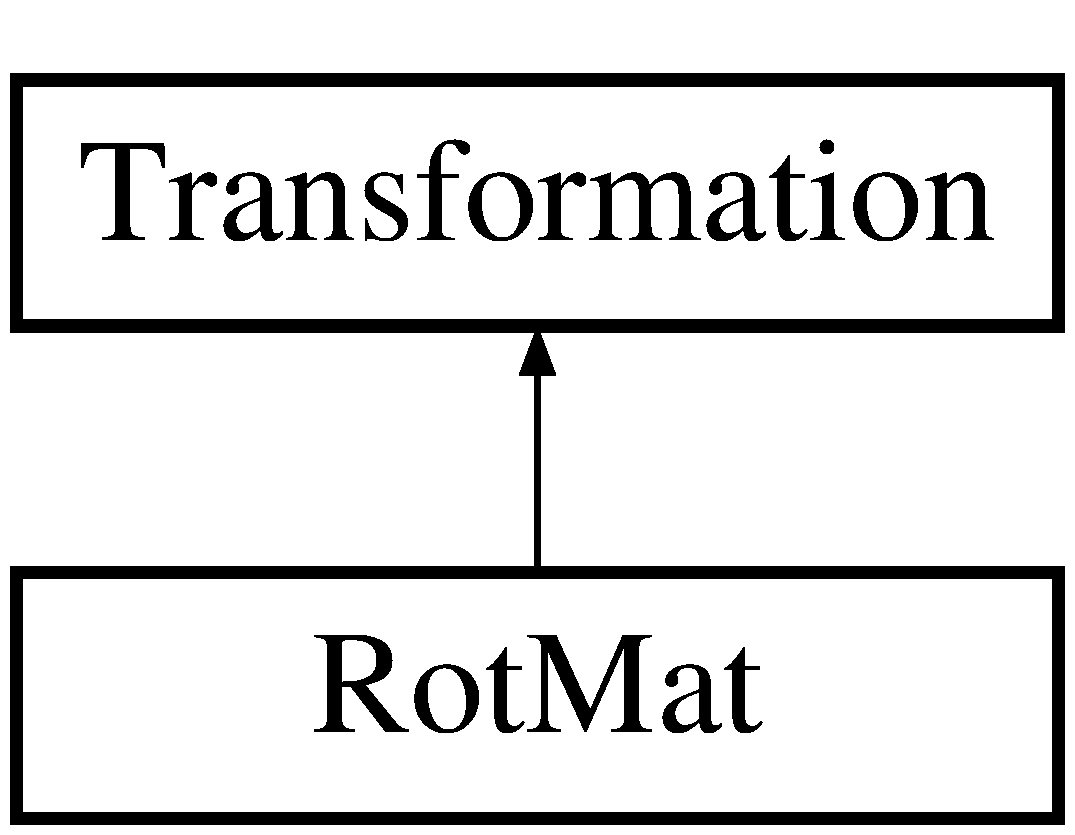
\includegraphics[height=2.000000cm]{class_rot_mat}
\end{center}
\end{figure}
\subsection*{Public Member Functions}
\begin{DoxyCompactItemize}
\item 
\hypertarget{class_rot_mat_abe1e5d870c095d4345d58d5539a3f86a}{const \hyperlink{class_rot_mat}{Rot\-Mat} \& {\bfseries Reset} (const \hyperlink{class_angel_1_1mat4}{Angel\-::mat4} \&New\-State)}\label{class_rot_mat_abe1e5d870c095d4345d58d5539a3f86a}

\item 
\hypertarget{class_rot_mat_ac6975ee8070d4477d86eb0e61482b7b6}{const \hyperlink{class_rot_mat}{Rot\-Mat} \& {\bfseries Rotate\-X} (const G\-Lfloat theta, bool order=true)}\label{class_rot_mat_ac6975ee8070d4477d86eb0e61482b7b6}

\item 
\hypertarget{class_rot_mat_a49c0d0cb066fd400bc51f1bd7822d36e}{const \hyperlink{class_rot_mat}{Rot\-Mat} \& {\bfseries Rotate\-Y} (const G\-Lfloat theta, bool order=true)}\label{class_rot_mat_a49c0d0cb066fd400bc51f1bd7822d36e}

\item 
\hypertarget{class_rot_mat_a04e786ea267f55f2b11f722f980e1440}{const \hyperlink{class_rot_mat}{Rot\-Mat} \& {\bfseries Rotate\-Z} (const G\-Lfloat theta, bool order=true)}\label{class_rot_mat_a04e786ea267f55f2b11f722f980e1440}

\item 
\hypertarget{class_rot_mat_a415534929361d6d78800aa7f4da2e6c7}{const \hyperlink{class_rot_mat}{Rot\-Mat} \& {\bfseries Adjust} (const \hyperlink{class_angel_1_1mat4}{Angel\-::mat4} \&Adjustment, bool order=true)}\label{class_rot_mat_a415534929361d6d78800aa7f4da2e6c7}

\item 
\hypertarget{class_transformation_ae6a57a1ee74ca1da1b8aef3d328a8772}{const \hyperlink{class_angel_1_1mat4}{Angel\-::mat4} \& {\bfseries Matrix} (void) const }\label{class_transformation_ae6a57a1ee74ca1da1b8aef3d328a8772}

\item 
\hypertarget{class_transformation_afdfbf48815a5b0d885f3b93f04cd2c66}{\hyperlink{class_angel_1_1mat4}{Angel\-::mat4} {\bfseries operator$\ast$} (const \hyperlink{class_angel_1_1mat4}{Angel\-::mat4} \&rhs) const }\label{class_transformation_afdfbf48815a5b0d885f3b93f04cd2c66}

\item 
\hypertarget{class_transformation_a85b923e0066365ef2e4aec3671396410}{\hyperlink{class_angel_1_1mat4}{Angel\-::mat4} {\bfseries operator$\ast$} (const \hyperlink{class_transformation}{Transformation} \&rhs) const }\label{class_transformation_a85b923e0066365ef2e4aec3671396410}

\end{DoxyCompactItemize}
\subsection*{Protected Attributes}
\begin{DoxyCompactItemize}
\item 
\hypertarget{class_transformation_a5f39fb578a1cdf78ca85efbd932d3834}{\hyperlink{class_angel_1_1mat4}{Angel\-::mat4} {\bfseries mat}}\label{class_transformation_a5f39fb578a1cdf78ca85efbd932d3834}

\end{DoxyCompactItemize}


\subsection{Detailed Description}
Rotations. 

Definition at line 33 of file Transformation.\-hpp.



The documentation for this class was generated from the following files\-:\begin{DoxyCompactItemize}
\item 
Transformation.\-hpp\item 
Transformation.\-cpp\end{DoxyCompactItemize}

\hypertarget{class_scale_mat}{\section{Scale\-Mat Class Reference}
\label{class_scale_mat}\index{Scale\-Mat@{Scale\-Mat}}
}
Inheritance diagram for Scale\-Mat\-:\begin{figure}[H]
\begin{center}
\leavevmode
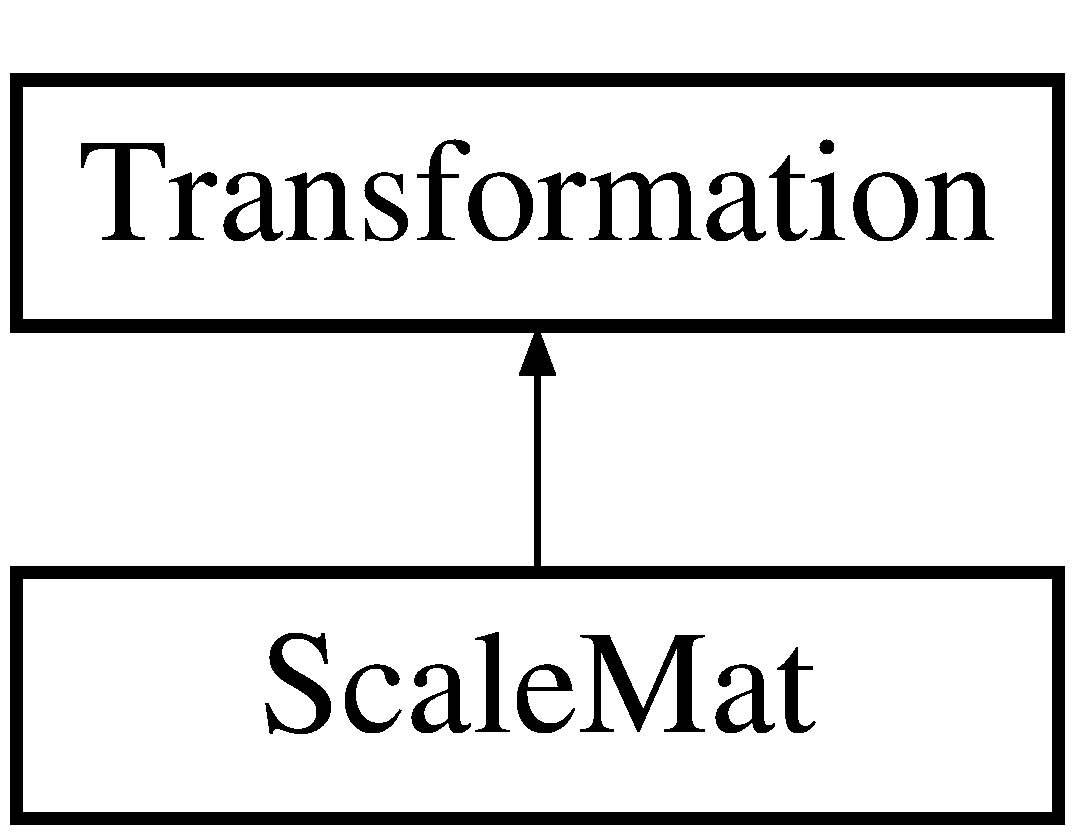
\includegraphics[height=2.000000cm]{class_scale_mat}
\end{center}
\end{figure}
\subsection*{Public Member Functions}
\begin{DoxyCompactItemize}
\item 
\hypertarget{class_scale_mat_aa72e3e61eddd0e88092e6cc76cc78972}{const \hyperlink{class_scale_mat}{Scale\-Mat} \& {\bfseries Set} (const float x, const float y, const float z)}\label{class_scale_mat_aa72e3e61eddd0e88092e6cc76cc78972}

\item 
\hypertarget{class_scale_mat_aea523b732204366c105809fc447ff07e}{const \hyperlink{class_scale_mat}{Scale\-Mat} \& {\bfseries Set} (const float pct)}\label{class_scale_mat_aea523b732204366c105809fc447ff07e}

\item 
\hypertarget{class_scale_mat_ad259370ba433114d9cdbd9d817552905}{const \hyperlink{class_scale_mat}{Scale\-Mat} \& {\bfseries Adjust} (const float x, const float y, const float z)}\label{class_scale_mat_ad259370ba433114d9cdbd9d817552905}

\item 
\hypertarget{class_scale_mat_af915563091d994e41c309a2bcd31615e}{const \hyperlink{class_scale_mat}{Scale\-Mat} \& {\bfseries Adjust} (const float pct)}\label{class_scale_mat_af915563091d994e41c309a2bcd31615e}

\item 
\hypertarget{class_transformation_ae6a57a1ee74ca1da1b8aef3d328a8772}{const \hyperlink{class_angel_1_1mat4}{Angel\-::mat4} \& {\bfseries Matrix} (void) const }\label{class_transformation_ae6a57a1ee74ca1da1b8aef3d328a8772}

\item 
\hypertarget{class_transformation_afdfbf48815a5b0d885f3b93f04cd2c66}{\hyperlink{class_angel_1_1mat4}{Angel\-::mat4} {\bfseries operator$\ast$} (const \hyperlink{class_angel_1_1mat4}{Angel\-::mat4} \&rhs) const }\label{class_transformation_afdfbf48815a5b0d885f3b93f04cd2c66}

\item 
\hypertarget{class_transformation_a85b923e0066365ef2e4aec3671396410}{\hyperlink{class_angel_1_1mat4}{Angel\-::mat4} {\bfseries operator$\ast$} (const \hyperlink{class_transformation}{Transformation} \&rhs) const }\label{class_transformation_a85b923e0066365ef2e4aec3671396410}

\end{DoxyCompactItemize}
\subsection*{Protected Attributes}
\begin{DoxyCompactItemize}
\item 
\hypertarget{class_transformation_a5f39fb578a1cdf78ca85efbd932d3834}{\hyperlink{class_angel_1_1mat4}{Angel\-::mat4} {\bfseries mat}}\label{class_transformation_a5f39fb578a1cdf78ca85efbd932d3834}

\end{DoxyCompactItemize}


\subsection{Detailed Description}


Definition at line 63 of file Transformation.\-hpp.



The documentation for this class was generated from the following files\-:\begin{DoxyCompactItemize}
\item 
Transformation.\-hpp\item 
Transformation.\-cpp\end{DoxyCompactItemize}

\hypertarget{class_scene}{\section{Scene Class Reference}
\label{class_scene}\index{Scene@{Scene}}
}
\subsection*{Public Member Functions}
\begin{DoxyCompactItemize}
\item 
\hypertarget{class_scene_a3010030e68d0468b8d18c1323e072e80}{void {\bfseries Set\-Shader} (G\-Luint g\-Shader)}\label{class_scene_a3010030e68d0468b8d18c1323e072e80}

\item 
\hypertarget{class_scene_a1183da422d278456867460fb11ac8dc8}{\hyperlink{class_object}{Object} $\ast$ {\bfseries Add\-Object} (std\-::string obj\-Name)}\label{class_scene_a1183da422d278456867460fb11ac8dc8}

\item 
\hypertarget{class_scene_a1643bca3e943c5865c0aecb037006f58}{void {\bfseries Del\-Object} (std\-::string obj\-Name)}\label{class_scene_a1643bca3e943c5865c0aecb037006f58}

\item 
\hypertarget{class_scene_a43fd3c56db5dc940d1724b9573c9a360}{void {\bfseries Del\-Object} (void)}\label{class_scene_a43fd3c56db5dc940d1724b9573c9a360}

\item 
\hypertarget{class_scene_abdfd15e7987aa261840d5ecc265170df}{void {\bfseries Pop\-Object} (void)}\label{class_scene_abdfd15e7987aa261840d5ecc265170df}

\item 
\hypertarget{class_scene_a0a57ee2c15864c55cf3284b937440330}{\hyperlink{class_object}{Object} $\ast$ {\bfseries Next} (void)}\label{class_scene_a0a57ee2c15864c55cf3284b937440330}

\item 
\hypertarget{class_scene_a955c5c984cc6bc5fb532752e43256211}{\hyperlink{class_object}{Object} $\ast$ {\bfseries Prev} (void)}\label{class_scene_a955c5c984cc6bc5fb532752e43256211}

\item 
\hypertarget{class_scene_a50f6c9e9aa2e243da5e86bf3470c809e}{\hyperlink{class_object}{Object} $\ast$ {\bfseries Active} (void)}\label{class_scene_a50f6c9e9aa2e243da5e86bf3470c809e}

\item 
\hypertarget{class_scene_ad5a91c929b569b9111061eec16b3febf}{void {\bfseries Draw} (void)}\label{class_scene_ad5a91c929b569b9111061eec16b3febf}

\end{DoxyCompactItemize}
\subsection*{Private Member Functions}
\begin{DoxyCompactItemize}
\item 
\hypertarget{class_scene_a54a7aee3ada3309584dd979bd82c159a}{{\bfseries Scene} (\hyperlink{class_scene}{Scene} \&copy)}\label{class_scene_a54a7aee3ada3309584dd979bd82c159a}

\item 
\hypertarget{class_scene_af43eeff7e8d0d450c68341c73f9b1ab4}{\hyperlink{class_scene}{Scene} \& {\bfseries operator=} (const \hyperlink{class_scene}{Scene} \&copy)}\label{class_scene_af43eeff7e8d0d450c68341c73f9b1ab4}

\item 
void \hyperlink{class_scene_a8bbe0e5b1bfc71034b18e240e86aa285}{Delete\-Object} (\hyperlink{class_object}{Object} $\ast$obj)
\begin{DoxyCompactList}\small\item\em Delete\-Object is the actual implementation function that will remove an \hyperlink{class_object}{Object} from the \hyperlink{class_scene}{Scene} list and \hyperlink{class_scene}{Scene} map, then free the object. \end{DoxyCompactList}\end{DoxyCompactItemize}
\subsection*{Private Attributes}
\begin{DoxyCompactItemize}
\item 
\hypertarget{class_scene_ad4f10706155e3e956fe36a4b5f0ef731}{std\-::map$<$ std\-::string, \hyperlink{class_object}{Object} $\ast$ $>$ {\bfseries map}}\label{class_scene_ad4f10706155e3e956fe36a4b5f0ef731}

\item 
\hypertarget{class_scene_ac04ab16dd305db619afe5f8ec6a02ebc}{std\-::list$<$ \hyperlink{class_object}{Object} $\ast$ $>$ {\bfseries list}}\label{class_scene_ac04ab16dd305db619afe5f8ec6a02ebc}

\item 
\hypertarget{class_scene_acbf527a005c67461e03d343a9f853807}{std\-::list$<$ \hyperlink{class_object}{Object} $\ast$ $>$\-::iterator {\bfseries current\-Obj}}\label{class_scene_acbf527a005c67461e03d343a9f853807}

\item 
\hypertarget{class_scene_aece20244e3987065f05057452a14d81f}{G\-Luint {\bfseries g\-Shader}}\label{class_scene_aece20244e3987065f05057452a14d81f}

\end{DoxyCompactItemize}


\subsection{Detailed Description}


Definition at line 8 of file Scene.\-hpp.



\subsection{Member Function Documentation}
\hypertarget{class_scene_a8bbe0e5b1bfc71034b18e240e86aa285}{\index{Scene@{Scene}!Delete\-Object@{Delete\-Object}}
\index{Delete\-Object@{Delete\-Object}!Scene@{Scene}}
\subsubsection[{Delete\-Object}]{\setlength{\rightskip}{0pt plus 5cm}void Scene\-::\-Delete\-Object (
\begin{DoxyParamCaption}
\item[{{\bf Object} $\ast$}]{obj}
\end{DoxyParamCaption}
)\hspace{0.3cm}{\ttfamily [private]}}}\label{class_scene_a8bbe0e5b1bfc71034b18e240e86aa285}


Delete\-Object is the actual implementation function that will remove an \hyperlink{class_object}{Object} from the \hyperlink{class_scene}{Scene} list and \hyperlink{class_scene}{Scene} map, then free the object. 


\begin{DoxyParams}{Parameters}
{\em obj} & The pointer to the object to free. \\
\hline
\end{DoxyParams}


Definition at line 37 of file Scene.\-cpp.



The documentation for this class was generated from the following files\-:\begin{DoxyCompactItemize}
\item 
Scene.\-hpp\item 
Scene.\-cpp\end{DoxyCompactItemize}

\hypertarget{class_screen}{\section{Screen Class Reference}
\label{class_screen}\index{Screen@{Screen}}
}
\subsection*{Public Member Functions}
\begin{DoxyCompactItemize}
\item 
\hypertarget{class_screen_ad664ad8b3ba858a4b9a3798cd2a0e295}{{\bfseries Screen} (int x, int y)}\label{class_screen_ad664ad8b3ba858a4b9a3798cd2a0e295}

\item 
\hypertarget{class_screen_a7b45282430392ffa8b5891936363f8f8}{{\bfseries Screen} (const \hyperlink{struct_angel_1_1vec2}{vec2} \&new\-Size)}\label{class_screen_a7b45282430392ffa8b5891936363f8f8}

\item 
\hypertarget{class_screen_a478c5176fd4fdc8af48f2bd7e824329d}{void {\bfseries Size} (int x, int y)}\label{class_screen_a478c5176fd4fdc8af48f2bd7e824329d}

\item 
\hypertarget{class_screen_a5fa4071af08df619e7cb4311bc0efb45}{void {\bfseries Size} (const \hyperlink{struct_angel_1_1vec2}{vec2} \&new\-Size)}\label{class_screen_a5fa4071af08df619e7cb4311bc0efb45}

\item 
\hypertarget{class_screen_a6f22423a037d9cf406d3ca4dd79b94b5}{const \hyperlink{struct_angel_1_1vec2}{vec2} \& {\bfseries Size} (void)}\label{class_screen_a6f22423a037d9cf406d3ca4dd79b94b5}

\item 
\hypertarget{class_screen_aa9a4a2e113af54d7164463bef8e78471}{int {\bfseries Width} (void)}\label{class_screen_aa9a4a2e113af54d7164463bef8e78471}

\item 
\hypertarget{class_screen_ad532ef57bbdb9a1e1540812a02eece23}{int {\bfseries Height} (void)}\label{class_screen_ad532ef57bbdb9a1e1540812a02eece23}

\item 
\hypertarget{class_screen_a00be376c569ac4b71d770f34e297f332}{const \hyperlink{struct_angel_1_1vec2}{vec2} \& {\bfseries Center} (void)}\label{class_screen_a00be376c569ac4b71d770f34e297f332}

\item 
\hypertarget{class_screen_a434f489a1b9d40319f7f6dbbf11db456}{int {\bfseries Midpoint\-X} (void)}\label{class_screen_a434f489a1b9d40319f7f6dbbf11db456}

\item 
\hypertarget{class_screen_a7b574e8ded50718dc1523180102e2f41}{int {\bfseries Midpoint\-Y} (void)}\label{class_screen_a7b574e8ded50718dc1523180102e2f41}

\end{DoxyCompactItemize}
\subsection*{Public Attributes}
\begin{DoxyCompactItemize}
\item 
\hypertarget{class_screen_ae18e2382eee3c792f94d251ee58b3264}{\hyperlink{class_cameras}{Cameras} {\bfseries cam\-List}}\label{class_screen_ae18e2382eee3c792f94d251ee58b3264}

\end{DoxyCompactItemize}
\subsection*{Private Attributes}
\begin{DoxyCompactItemize}
\item 
\hypertarget{class_screen_a518fc6d0287e8d3cf44a1eb73f3be6e7}{\hyperlink{struct_angel_1_1vec2}{vec2} {\bfseries size}}\label{class_screen_a518fc6d0287e8d3cf44a1eb73f3be6e7}

\item 
\hypertarget{class_screen_a9aaa9c66b706c2186fa024bf139078f3}{\hyperlink{struct_angel_1_1vec2}{vec2} {\bfseries center}}\label{class_screen_a9aaa9c66b706c2186fa024bf139078f3}

\end{DoxyCompactItemize}


\subsection{Detailed Description}


Definition at line 8 of file Screen.\-hpp.



The documentation for this class was generated from the following files\-:\begin{DoxyCompactItemize}
\item 
Screen.\-hpp\item 
Screen.\-cpp\end{DoxyCompactItemize}

\hypertarget{class_timer}{\section{Timer Class Reference}
\label{class_timer}\index{Timer@{Timer}}
}
\subsection*{Public Member Functions}
\begin{DoxyCompactItemize}
\item 
unsigned long \hyperlink{class_timer_a4e69d3c5a312d1b29d1735b2c5bccefb}{Tick} ()
\begin{DoxyCompactList}\small\item\em Tick is an alias for Tock. \end{DoxyCompactList}\item 
unsigned long \hyperlink{class_timer_a2c58a2e04e1e30926805aa4e82d2a0a5}{Tock} ()
\begin{DoxyCompactList}\small\item\em Tock returns the time elapsed since the last Tock. \end{DoxyCompactList}\item 
unsigned long \hyperlink{class_timer_a4f68da5b62cb1d1b2dd0c8549eb6286d}{Delta} () const 
\begin{DoxyCompactList}\small\item\em Delta returns the time elapsed between the last Tick and the last Tock. \end{DoxyCompactList}\item 
double \hyperlink{class_timer_a25ed035b0da5b177050c922660acf864}{Scale} () const 
\begin{DoxyCompactList}\small\item\em Scale returns the relative lateness or eagerness of the \hyperlink{class_timer}{Timer}, Relative to a benchmark or Key Frame Rate (The default is 60\-F\-P\-S, or 16667 msec.) \end{DoxyCompactList}\end{DoxyCompactItemize}
\subsection*{Private Attributes}
\begin{DoxyCompactItemize}
\item 
\hypertarget{class_timer_a384a34d671fa58160f0ea13713645462}{struct timeval {\bfseries \-\_\-\-T1}}\label{class_timer_a384a34d671fa58160f0ea13713645462}

\item 
\hypertarget{class_timer_a22691ac7f27eed709461091c1125d931}{struct timeval {\bfseries \-\_\-\-T2}}\label{class_timer_a22691ac7f27eed709461091c1125d931}

\item 
\hypertarget{class_timer_a3ded2a527b99c1fd983ea9583a7ebcdb}{unsigned long {\bfseries delta}}\label{class_timer_a3ded2a527b99c1fd983ea9583a7ebcdb}

\item 
\hypertarget{class_timer_a5d8edd0ebb4a43487733e9df2d5b6865}{double {\bfseries scale}}\label{class_timer_a5d8edd0ebb4a43487733e9df2d5b6865}

\end{DoxyCompactItemize}


\subsection{Detailed Description}


Definition at line 6 of file Timer.\-hpp.



\subsection{Member Function Documentation}
\hypertarget{class_timer_a4f68da5b62cb1d1b2dd0c8549eb6286d}{\index{Timer@{Timer}!Delta@{Delta}}
\index{Delta@{Delta}!Timer@{Timer}}
\subsubsection[{Delta}]{\setlength{\rightskip}{0pt plus 5cm}unsigned long Timer\-::\-Delta (
\begin{DoxyParamCaption}
\item[{void}]{}
\end{DoxyParamCaption}
) const}}\label{class_timer_a4f68da5b62cb1d1b2dd0c8549eb6286d}


Delta returns the time elapsed between the last Tick and the last Tock. 

Does not start a new timer. \begin{DoxyReturn}{Returns}
Time elapsed in Microseconds, or Nanoseconds if \-\_\-\-R\-T was enabled. 
\end{DoxyReturn}


Definition at line 58 of file Timer.\-cpp.

\hypertarget{class_timer_a25ed035b0da5b177050c922660acf864}{\index{Timer@{Timer}!Scale@{Scale}}
\index{Scale@{Scale}!Timer@{Timer}}
\subsubsection[{Scale}]{\setlength{\rightskip}{0pt plus 5cm}double Timer\-::\-Scale (
\begin{DoxyParamCaption}
\item[{void}]{}
\end{DoxyParamCaption}
) const}}\label{class_timer_a25ed035b0da5b177050c922660acf864}


Scale returns the relative lateness or eagerness of the \hyperlink{class_timer}{Timer}, Relative to a benchmark or Key Frame Rate (The default is 60\-F\-P\-S, or 16667 msec.) 

\begin{DoxyReturn}{Returns}
A non-\/zero float that ranges from (0,1) indicating that the program is rendering faster than 60\-F\-P\-S, or from the range \mbox{[}1,+inf) indicating that the program is rendering slower than 60\-F\-P\-S. 
\end{DoxyReturn}


Definition at line 72 of file Timer.\-cpp.

\hypertarget{class_timer_a4e69d3c5a312d1b29d1735b2c5bccefb}{\index{Timer@{Timer}!Tick@{Tick}}
\index{Tick@{Tick}!Timer@{Timer}}
\subsubsection[{Tick}]{\setlength{\rightskip}{0pt plus 5cm}unsigned long Timer\-::\-Tick (
\begin{DoxyParamCaption}
\item[{void}]{}
\end{DoxyParamCaption}
)}}\label{class_timer_a4e69d3c5a312d1b29d1735b2c5bccefb}


Tick is an alias for Tock. 

Ha, Ha, Ha. \begin{DoxyReturn}{Returns}
An unsigned long corresponding to how much time has passed since the last Tick. Microseconds normally, Nanoseconds if \-\_\-\-R\-T was enabled. 
\end{DoxyReturn}


Definition at line 29 of file Timer.\-cpp.

\hypertarget{class_timer_a2c58a2e04e1e30926805aa4e82d2a0a5}{\index{Timer@{Timer}!Tock@{Tock}}
\index{Tock@{Tock}!Timer@{Timer}}
\subsubsection[{Tock}]{\setlength{\rightskip}{0pt plus 5cm}unsigned long Timer\-::\-Tock (
\begin{DoxyParamCaption}
\item[{void}]{}
\end{DoxyParamCaption}
)}}\label{class_timer_a2c58a2e04e1e30926805aa4e82d2a0a5}


Tock returns the time elapsed since the last Tock. 

\begin{DoxyReturn}{Returns}
An unsigned long corresponding to how much time has passed since the last Tock. Microseconds normally, Nanoseconds if \-\_\-\-R\-T was enabled. 
\end{DoxyReturn}


Definition at line 39 of file Timer.\-cpp.



The documentation for this class was generated from the following files\-:\begin{DoxyCompactItemize}
\item 
Timer.\-hpp\item 
Timer.\-cpp\end{DoxyCompactItemize}

\hypertarget{class_trans_cache}{\section{Trans\-Cache Class Reference}
\label{class_trans_cache}\index{Trans\-Cache@{Trans\-Cache}}
}
\subsection*{Public Member Functions}
\begin{DoxyCompactItemize}
\item 
\hypertarget{class_trans_cache_a3a7d869c5a99b33f10c0e74ac082cfb4}{void {\bfseries P\-T\-M} (const \hyperlink{class_angel_1_1mat4}{Angel\-::mat4} \&ptm\-\_\-in)}\label{class_trans_cache_a3a7d869c5a99b33f10c0e74ac082cfb4}

\item 
\hypertarget{class_trans_cache_a7b425ff8ded5fb458e21ab4660785038}{const \hyperlink{class_angel_1_1mat4}{Angel\-::mat4} \& {\bfseries P\-T\-M} (void) const }\label{class_trans_cache_a7b425ff8ded5fb458e21ab4660785038}

\item 
\hypertarget{class_trans_cache_ac9396813c4f26840c9c5e825d2a56fef}{const \hyperlink{class_angel_1_1mat4}{Angel\-::mat4} \& {\bfseries C\-T\-M} (void) const }\label{class_trans_cache_ac9396813c4f26840c9c5e825d2a56fef}

\item 
\hypertarget{class_trans_cache_ac1ca33b96c384988bb7a46a250d441bd}{const \hyperlink{class_angel_1_1mat4}{Angel\-::mat4} \& {\bfseries O\-T\-M} (void) const }\label{class_trans_cache_ac1ca33b96c384988bb7a46a250d441bd}

\item 
\hypertarget{class_trans_cache_ac197a0d239be72c6c620bfe002f3880b}{void {\bfseries Calc\-C\-T\-M} (void)}\label{class_trans_cache_ac197a0d239be72c6c620bfe002f3880b}

\end{DoxyCompactItemize}
\subsection*{Public Attributes}
\begin{DoxyCompactItemize}
\item 
\hypertarget{class_trans_cache_a084f46900c69be0ba49b251edae90919}{\hyperlink{class_trans_mat}{Trans\-Mat} {\bfseries Pre\-Offset}}\label{class_trans_cache_a084f46900c69be0ba49b251edae90919}

\item 
\hypertarget{class_trans_cache_a0d9a476e9640885c8b06d23a517cb32d}{\hyperlink{class_scale_mat}{Scale\-Mat} {\bfseries scale}}\label{class_trans_cache_a0d9a476e9640885c8b06d23a517cb32d}

\item 
\hypertarget{class_trans_cache_aaf226f57f43c89c20a57ab0103acf581}{\hyperlink{class_rot_mat}{Rot\-Mat} {\bfseries rotation}}\label{class_trans_cache_aaf226f57f43c89c20a57ab0103acf581}

\item 
\hypertarget{class_trans_cache_a447c3b57cb43476f866a748bbd7003f1}{\hyperlink{class_trans_mat}{Trans\-Mat} {\bfseries offset}}\label{class_trans_cache_a447c3b57cb43476f866a748bbd7003f1}

\item 
\hypertarget{class_trans_cache_a0dd39219d23e23e0a0038b3a526fdb2b}{\hyperlink{class_rot_mat}{Rot\-Mat} {\bfseries orbit}}\label{class_trans_cache_a0dd39219d23e23e0a0038b3a526fdb2b}

\item 
\hypertarget{class_trans_cache_a23570257c2a224ace589c6f22dbfc135}{\hyperlink{class_trans_mat}{Trans\-Mat} {\bfseries displacement}}\label{class_trans_cache_a23570257c2a224ace589c6f22dbfc135}

\end{DoxyCompactItemize}
\subsection*{Private Attributes}
\begin{DoxyCompactItemize}
\item 
\hypertarget{class_trans_cache_af0652a8016db75eea63d9486ca1959ad}{\hyperlink{class_angel_1_1mat4}{Angel\-::mat4} {\bfseries ptm}}\label{class_trans_cache_af0652a8016db75eea63d9486ca1959ad}

\item 
\hypertarget{class_trans_cache_add771d1088642aca16cea5df82c1b6b0}{\hyperlink{class_angel_1_1mat4}{Angel\-::mat4} {\bfseries ctm}}\label{class_trans_cache_add771d1088642aca16cea5df82c1b6b0}

\item 
\hypertarget{class_trans_cache_afcebdcb61bebb8d44d40fa2d19d7009d}{\hyperlink{class_angel_1_1mat4}{Angel\-::mat4} {\bfseries otm}}\label{class_trans_cache_afcebdcb61bebb8d44d40fa2d19d7009d}

\end{DoxyCompactItemize}


\subsection{Detailed Description}


Definition at line 4 of file Trans\-Cache.\-hpp.



The documentation for this class was generated from the following files\-:\begin{DoxyCompactItemize}
\item 
Trans\-Cache.\-hpp\item 
Trans\-Cache.\-cpp\end{DoxyCompactItemize}

\hypertarget{class_transformation}{\section{Transformation Class Reference}
\label{class_transformation}\index{Transformation@{Transformation}}
}
Inheritance diagram for Transformation\-:\begin{figure}[H]
\begin{center}
\leavevmode
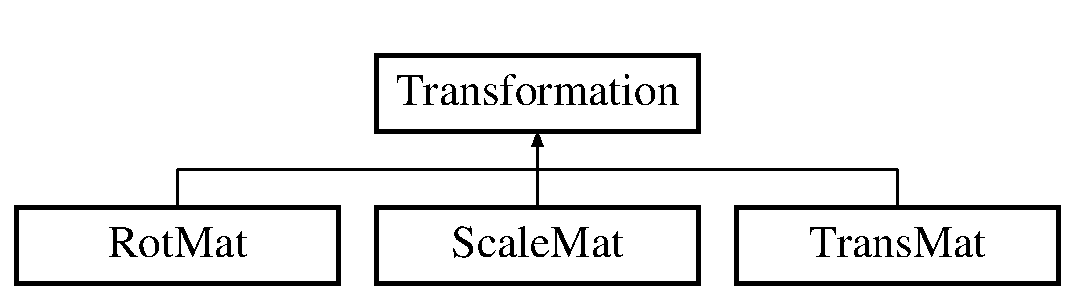
\includegraphics[height=2.000000cm]{class_transformation}
\end{center}
\end{figure}
\subsection*{Public Member Functions}
\begin{DoxyCompactItemize}
\item 
\hypertarget{class_transformation_ae6a57a1ee74ca1da1b8aef3d328a8772}{const \hyperlink{class_angel_1_1mat4}{Angel\-::mat4} \& {\bfseries Matrix} (void) const }\label{class_transformation_ae6a57a1ee74ca1da1b8aef3d328a8772}

\item 
\hypertarget{class_transformation_afdfbf48815a5b0d885f3b93f04cd2c66}{\hyperlink{class_angel_1_1mat4}{Angel\-::mat4} {\bfseries operator$\ast$} (const \hyperlink{class_angel_1_1mat4}{Angel\-::mat4} \&rhs) const }\label{class_transformation_afdfbf48815a5b0d885f3b93f04cd2c66}

\item 
\hypertarget{class_transformation_a85b923e0066365ef2e4aec3671396410}{\hyperlink{class_angel_1_1mat4}{Angel\-::mat4} {\bfseries operator$\ast$} (const \hyperlink{class_transformation}{Transformation} \&rhs) const }\label{class_transformation_a85b923e0066365ef2e4aec3671396410}

\end{DoxyCompactItemize}
\subsection*{Protected Attributes}
\begin{DoxyCompactItemize}
\item 
\hypertarget{class_transformation_a5f39fb578a1cdf78ca85efbd932d3834}{\hyperlink{class_angel_1_1mat4}{Angel\-::mat4} {\bfseries mat}}\label{class_transformation_a5f39fb578a1cdf78ca85efbd932d3834}

\end{DoxyCompactItemize}


\subsection{Detailed Description}


Definition at line 8 of file Transformation.\-hpp.



The documentation for this class was generated from the following files\-:\begin{DoxyCompactItemize}
\item 
Transformation.\-hpp\item 
Transformation.\-cpp\end{DoxyCompactItemize}

\hypertarget{class_trans_mat}{\section{Trans\-Mat Class Reference}
\label{class_trans_mat}\index{Trans\-Mat@{Trans\-Mat}}
}


Translations.  




{\ttfamily \#include $<$Transformation.\-hpp$>$}

Inheritance diagram for Trans\-Mat\-:\begin{figure}[H]
\begin{center}
\leavevmode
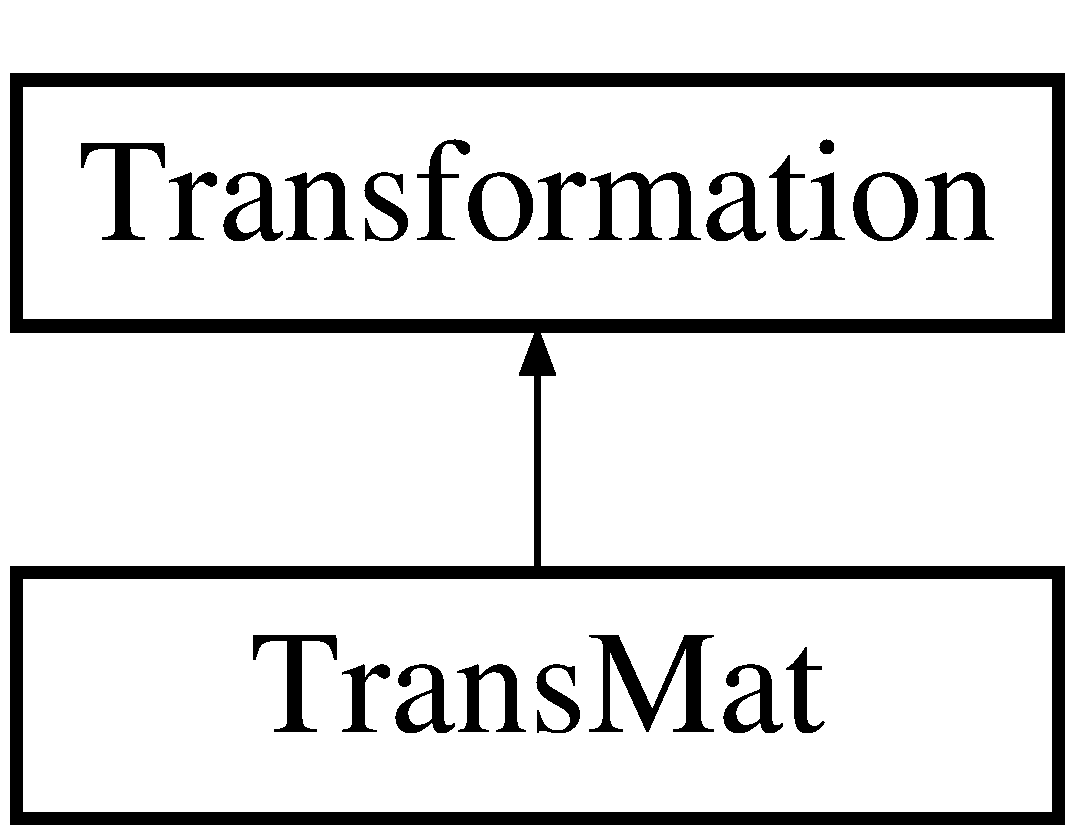
\includegraphics[height=2.000000cm]{class_trans_mat}
\end{center}
\end{figure}
\subsection*{Public Member Functions}
\begin{DoxyCompactItemize}
\item 
\hypertarget{class_trans_mat_a0a06e0dbfa09be06f0b8057283904b61}{const \hyperlink{class_trans_mat}{Trans\-Mat} \& {\bfseries Set\-X} (const float x)}\label{class_trans_mat_a0a06e0dbfa09be06f0b8057283904b61}

\item 
\hypertarget{class_trans_mat_a06c565961177be6b4945899d099eb7bc}{const \hyperlink{class_trans_mat}{Trans\-Mat} \& {\bfseries Set\-Y} (const float y)}\label{class_trans_mat_a06c565961177be6b4945899d099eb7bc}

\item 
\hypertarget{class_trans_mat_a9eaca6a2622a5820ee996409c477a54e}{const \hyperlink{class_trans_mat}{Trans\-Mat} \& {\bfseries Set\-Z} (const float z)}\label{class_trans_mat_a9eaca6a2622a5820ee996409c477a54e}

\item 
\hypertarget{class_trans_mat_a674c38b07b3f30ca46fdad9b3e699b77}{const \hyperlink{class_trans_mat}{Trans\-Mat} \& {\bfseries Set} (const float x, const float y, const float z)}\label{class_trans_mat_a674c38b07b3f30ca46fdad9b3e699b77}

\item 
\hypertarget{class_trans_mat_a5d6ab266be86788df753e5457afbe461}{const \hyperlink{class_trans_mat}{Trans\-Mat} \& {\bfseries Set} (const \hyperlink{struct_angel_1_1vec3}{Angel\-::vec3} \&arg)}\label{class_trans_mat_a5d6ab266be86788df753e5457afbe461}

\item 
\hypertarget{class_trans_mat_acaca3bb158b497ae5924fda662ff324d}{const \hyperlink{class_trans_mat}{Trans\-Mat} \& {\bfseries Delta} (const float x, const float y, const float z)}\label{class_trans_mat_acaca3bb158b497ae5924fda662ff324d}

\item 
\hypertarget{class_trans_mat_a1ba9395450677744c7c86d98f2d094d8}{const \hyperlink{class_trans_mat}{Trans\-Mat} \& {\bfseries Delta} (const \hyperlink{struct_angel_1_1vec3}{Angel\-::vec3} \&arg)}\label{class_trans_mat_a1ba9395450677744c7c86d98f2d094d8}

\item 
\hypertarget{class_transformation_ae6a57a1ee74ca1da1b8aef3d328a8772}{const \hyperlink{class_angel_1_1mat4}{Angel\-::mat4} \& {\bfseries Matrix} (void) const }\label{class_transformation_ae6a57a1ee74ca1da1b8aef3d328a8772}

\item 
\hypertarget{class_transformation_afdfbf48815a5b0d885f3b93f04cd2c66}{\hyperlink{class_angel_1_1mat4}{Angel\-::mat4} {\bfseries operator$\ast$} (const \hyperlink{class_angel_1_1mat4}{Angel\-::mat4} \&rhs) const }\label{class_transformation_afdfbf48815a5b0d885f3b93f04cd2c66}

\item 
\hypertarget{class_transformation_a85b923e0066365ef2e4aec3671396410}{\hyperlink{class_angel_1_1mat4}{Angel\-::mat4} {\bfseries operator$\ast$} (const \hyperlink{class_transformation}{Transformation} \&rhs) const }\label{class_transformation_a85b923e0066365ef2e4aec3671396410}

\end{DoxyCompactItemize}
\subsection*{Protected Attributes}
\begin{DoxyCompactItemize}
\item 
\hypertarget{class_transformation_a5f39fb578a1cdf78ca85efbd932d3834}{\hyperlink{class_angel_1_1mat4}{Angel\-::mat4} {\bfseries mat}}\label{class_transformation_a5f39fb578a1cdf78ca85efbd932d3834}

\end{DoxyCompactItemize}


\subsection{Detailed Description}
Translations. 

Definition at line 47 of file Transformation.\-hpp.



The documentation for this class was generated from the following files\-:\begin{DoxyCompactItemize}
\item 
Transformation.\-hpp\item 
Transformation.\-cpp\end{DoxyCompactItemize}

\hypertarget{classtxload}{\section{txload Class Reference}
\label{classtxload}\index{txload@{txload}}
}
\subsection*{Public Member Functions}
\begin{DoxyCompactItemize}
\item 
\hypertarget{classtxload_ab9da9ed1b71d2ddaab7df3ed889525eb}{{\bfseries txload} (const char $\ast$filename, G\-Luint Text\-Enum, G\-Luint g\-Shader, const char $\ast$uniform, int num)}\label{classtxload_ab9da9ed1b71d2ddaab7df3ed889525eb}

\end{DoxyCompactItemize}
\subsection*{Public Attributes}
\begin{DoxyCompactItemize}
\item 
\hypertarget{classtxload_a3bf11d886fa0b9d9cdb96f1dbb50a7fa}{const char $\ast$ {\bfseries filename}}\label{classtxload_a3bf11d886fa0b9d9cdb96f1dbb50a7fa}

\item 
\hypertarget{classtxload_a434622c4f197b65c8121c3babc332d7d}{G\-Luint {\bfseries Text\-Enum}}\label{classtxload_a434622c4f197b65c8121c3babc332d7d}

\item 
\hypertarget{classtxload_a6d71f2bdca8e995e88a7c0e9cc9dfa47}{G\-Luint {\bfseries g\-Shader}}\label{classtxload_a6d71f2bdca8e995e88a7c0e9cc9dfa47}

\item 
\hypertarget{classtxload_a23aee3e0e6f6847c75b777f6e8825c3e}{const char $\ast$ {\bfseries uniform}}\label{classtxload_a23aee3e0e6f6847c75b777f6e8825c3e}

\item 
\hypertarget{classtxload_a7173d10b57d5d095b0deb0857d163055}{int {\bfseries num}}\label{classtxload_a7173d10b57d5d095b0deb0857d163055}

\end{DoxyCompactItemize}


\subsection{Detailed Description}


Definition at line 5 of file Load\-Texture.\-hpp.



The documentation for this class was generated from the following files\-:\begin{DoxyCompactItemize}
\item 
Load\-Texture.\-hpp\item 
Load\-Texture.\-cpp\end{DoxyCompactItemize}

\hypertarget{struct_angel_1_1vec2}{\section{\-Angel\-:\-:vec2 \-Struct \-Reference}
\label{struct_angel_1_1vec2}\index{\-Angel\-::vec2@{\-Angel\-::vec2}}
}
\subsection*{\-Public \-Member \-Functions}
\begin{DoxyCompactItemize}
\item 
\hypertarget{struct_angel_1_1vec2_ab2463ddb6aaaa67251004b90f03530fa}{{\bfseries vec2} (\-G\-Lfloat s=\-G\-Lfloat(0.\-0))}\label{struct_angel_1_1vec2_ab2463ddb6aaaa67251004b90f03530fa}

\item 
\hypertarget{struct_angel_1_1vec2_a8e55cc0bb681ca7a747721cab122d830}{{\bfseries vec2} (\-G\-Lfloat x, \-G\-Lfloat y)}\label{struct_angel_1_1vec2_a8e55cc0bb681ca7a747721cab122d830}

\item 
\hypertarget{struct_angel_1_1vec2_aa2ec5b81c4b97019486b0595db6f35a1}{{\bfseries vec2} (const \hyperlink{struct_angel_1_1vec2}{vec2} \&v)}\label{struct_angel_1_1vec2_aa2ec5b81c4b97019486b0595db6f35a1}

\item 
\hypertarget{struct_angel_1_1vec2_a2605b81b6230d8d9184f3a06ff3fe7ae}{\-G\-Lfloat \& {\bfseries operator\mbox{[}$\,$\mbox{]}} (int i)}\label{struct_angel_1_1vec2_a2605b81b6230d8d9184f3a06ff3fe7ae}

\item 
\hypertarget{struct_angel_1_1vec2_a83725a082bca8ea73a2171bb4596c1bd}{const \-G\-Lfloat {\bfseries operator\mbox{[}$\,$\mbox{]}} (int i) const }\label{struct_angel_1_1vec2_a83725a082bca8ea73a2171bb4596c1bd}

\item 
\hypertarget{struct_angel_1_1vec2_a3b29693925c8026f75572dd13cefee5a}{\hyperlink{struct_angel_1_1vec2}{vec2} {\bfseries operator-\/} () const }\label{struct_angel_1_1vec2_a3b29693925c8026f75572dd13cefee5a}

\item 
\hypertarget{struct_angel_1_1vec2_a93606208e7b65d4bb8004f498b22934f}{\hyperlink{struct_angel_1_1vec2}{vec2} {\bfseries operator+} (const \hyperlink{struct_angel_1_1vec2}{vec2} \&v) const }\label{struct_angel_1_1vec2_a93606208e7b65d4bb8004f498b22934f}

\item 
\hypertarget{struct_angel_1_1vec2_a2d3d52e1b4693fdb860c2ef246e0d4d8}{\hyperlink{struct_angel_1_1vec2}{vec2} {\bfseries operator-\/} (const \hyperlink{struct_angel_1_1vec2}{vec2} \&v) const }\label{struct_angel_1_1vec2_a2d3d52e1b4693fdb860c2ef246e0d4d8}

\item 
\hypertarget{struct_angel_1_1vec2_ac5615b2494e3f8824f9fa127ba122b67}{\hyperlink{struct_angel_1_1vec2}{vec2} {\bfseries operator$\ast$} (const \-G\-Lfloat s) const }\label{struct_angel_1_1vec2_ac5615b2494e3f8824f9fa127ba122b67}

\item 
\hypertarget{struct_angel_1_1vec2_a3b4a9670b53342b870e3a14c8164c613}{\hyperlink{struct_angel_1_1vec2}{vec2} {\bfseries operator$\ast$} (const \hyperlink{struct_angel_1_1vec2}{vec2} \&v) const }\label{struct_angel_1_1vec2_a3b4a9670b53342b870e3a14c8164c613}

\item 
\hypertarget{struct_angel_1_1vec2_a522a6aaa64c361b86f6c2469cbd8ca92}{\hyperlink{struct_angel_1_1vec2}{vec2} {\bfseries operator/} (const \-G\-Lfloat s) const }\label{struct_angel_1_1vec2_a522a6aaa64c361b86f6c2469cbd8ca92}

\item 
\hypertarget{struct_angel_1_1vec2_a0d7255e85aa7765f6e54160c2f6d6d40}{\hyperlink{struct_angel_1_1vec2}{vec2} \& {\bfseries operator+=} (const \hyperlink{struct_angel_1_1vec2}{vec2} \&v)}\label{struct_angel_1_1vec2_a0d7255e85aa7765f6e54160c2f6d6d40}

\item 
\hypertarget{struct_angel_1_1vec2_ad650808486497a53572561c664c6e865}{\hyperlink{struct_angel_1_1vec2}{vec2} \& {\bfseries operator-\/=} (const \hyperlink{struct_angel_1_1vec2}{vec2} \&v)}\label{struct_angel_1_1vec2_ad650808486497a53572561c664c6e865}

\item 
\hypertarget{struct_angel_1_1vec2_afb79fcf6de3814fd875d1402e160097a}{\hyperlink{struct_angel_1_1vec2}{vec2} \& {\bfseries operator$\ast$=} (const \-G\-Lfloat s)}\label{struct_angel_1_1vec2_afb79fcf6de3814fd875d1402e160097a}

\item 
\hypertarget{struct_angel_1_1vec2_aa13326415630734f076da6e7466ea195}{\hyperlink{struct_angel_1_1vec2}{vec2} \& {\bfseries operator$\ast$=} (const \hyperlink{struct_angel_1_1vec2}{vec2} \&v)}\label{struct_angel_1_1vec2_aa13326415630734f076da6e7466ea195}

\item 
\hypertarget{struct_angel_1_1vec2_a0739a7464b89dc5b40fae5c423711e11}{\hyperlink{struct_angel_1_1vec2}{vec2} \& {\bfseries operator/=} (const \-G\-Lfloat s)}\label{struct_angel_1_1vec2_a0739a7464b89dc5b40fae5c423711e11}

\item 
\hypertarget{struct_angel_1_1vec2_a5c3d2082bcc18734fde3689dbc605104}{{\bfseries operator const G\-Lfloat $\ast$} () const }\label{struct_angel_1_1vec2_a5c3d2082bcc18734fde3689dbc605104}

\item 
\hypertarget{struct_angel_1_1vec2_a8989f46bc38bb87bc2f6ea81f66c8545}{{\bfseries operator G\-Lfloat $\ast$} ()}\label{struct_angel_1_1vec2_a8989f46bc38bb87bc2f6ea81f66c8545}

\item 
\hypertarget{struct_angel_1_1vec2_ab2463ddb6aaaa67251004b90f03530fa}{{\bfseries vec2} (\-G\-Lfloat s=\-G\-Lfloat(0.\-0))}\label{struct_angel_1_1vec2_ab2463ddb6aaaa67251004b90f03530fa}

\item 
\hypertarget{struct_angel_1_1vec2_a8e55cc0bb681ca7a747721cab122d830}{{\bfseries vec2} (\-G\-Lfloat x, \-G\-Lfloat y)}\label{struct_angel_1_1vec2_a8e55cc0bb681ca7a747721cab122d830}

\item 
\hypertarget{struct_angel_1_1vec2_aa2ec5b81c4b97019486b0595db6f35a1}{{\bfseries vec2} (const \hyperlink{struct_angel_1_1vec2}{vec2} \&v)}\label{struct_angel_1_1vec2_aa2ec5b81c4b97019486b0595db6f35a1}

\item 
\hypertarget{struct_angel_1_1vec2_a2605b81b6230d8d9184f3a06ff3fe7ae}{\-G\-Lfloat \& {\bfseries operator\mbox{[}$\,$\mbox{]}} (int i)}\label{struct_angel_1_1vec2_a2605b81b6230d8d9184f3a06ff3fe7ae}

\item 
\hypertarget{struct_angel_1_1vec2_a83725a082bca8ea73a2171bb4596c1bd}{const \-G\-Lfloat {\bfseries operator\mbox{[}$\,$\mbox{]}} (int i) const }\label{struct_angel_1_1vec2_a83725a082bca8ea73a2171bb4596c1bd}

\item 
\hypertarget{struct_angel_1_1vec2_a3b29693925c8026f75572dd13cefee5a}{\hyperlink{struct_angel_1_1vec2}{vec2} {\bfseries operator-\/} () const }\label{struct_angel_1_1vec2_a3b29693925c8026f75572dd13cefee5a}

\item 
\hypertarget{struct_angel_1_1vec2_a93606208e7b65d4bb8004f498b22934f}{\hyperlink{struct_angel_1_1vec2}{vec2} {\bfseries operator+} (const \hyperlink{struct_angel_1_1vec2}{vec2} \&v) const }\label{struct_angel_1_1vec2_a93606208e7b65d4bb8004f498b22934f}

\item 
\hypertarget{struct_angel_1_1vec2_a2d3d52e1b4693fdb860c2ef246e0d4d8}{\hyperlink{struct_angel_1_1vec2}{vec2} {\bfseries operator-\/} (const \hyperlink{struct_angel_1_1vec2}{vec2} \&v) const }\label{struct_angel_1_1vec2_a2d3d52e1b4693fdb860c2ef246e0d4d8}

\item 
\hypertarget{struct_angel_1_1vec2_ac5615b2494e3f8824f9fa127ba122b67}{\hyperlink{struct_angel_1_1vec2}{vec2} {\bfseries operator$\ast$} (const \-G\-Lfloat s) const }\label{struct_angel_1_1vec2_ac5615b2494e3f8824f9fa127ba122b67}

\item 
\hypertarget{struct_angel_1_1vec2_a3b4a9670b53342b870e3a14c8164c613}{\hyperlink{struct_angel_1_1vec2}{vec2} {\bfseries operator$\ast$} (const \hyperlink{struct_angel_1_1vec2}{vec2} \&v) const }\label{struct_angel_1_1vec2_a3b4a9670b53342b870e3a14c8164c613}

\item 
\hypertarget{struct_angel_1_1vec2_a522a6aaa64c361b86f6c2469cbd8ca92}{\hyperlink{struct_angel_1_1vec2}{vec2} {\bfseries operator/} (const \-G\-Lfloat s) const }\label{struct_angel_1_1vec2_a522a6aaa64c361b86f6c2469cbd8ca92}

\item 
\hypertarget{struct_angel_1_1vec2_a0d7255e85aa7765f6e54160c2f6d6d40}{\hyperlink{struct_angel_1_1vec2}{vec2} \& {\bfseries operator+=} (const \hyperlink{struct_angel_1_1vec2}{vec2} \&v)}\label{struct_angel_1_1vec2_a0d7255e85aa7765f6e54160c2f6d6d40}

\item 
\hypertarget{struct_angel_1_1vec2_ad650808486497a53572561c664c6e865}{\hyperlink{struct_angel_1_1vec2}{vec2} \& {\bfseries operator-\/=} (const \hyperlink{struct_angel_1_1vec2}{vec2} \&v)}\label{struct_angel_1_1vec2_ad650808486497a53572561c664c6e865}

\item 
\hypertarget{struct_angel_1_1vec2_afb79fcf6de3814fd875d1402e160097a}{\hyperlink{struct_angel_1_1vec2}{vec2} \& {\bfseries operator$\ast$=} (const \-G\-Lfloat s)}\label{struct_angel_1_1vec2_afb79fcf6de3814fd875d1402e160097a}

\item 
\hypertarget{struct_angel_1_1vec2_aa13326415630734f076da6e7466ea195}{\hyperlink{struct_angel_1_1vec2}{vec2} \& {\bfseries operator$\ast$=} (const \hyperlink{struct_angel_1_1vec2}{vec2} \&v)}\label{struct_angel_1_1vec2_aa13326415630734f076da6e7466ea195}

\item 
\hypertarget{struct_angel_1_1vec2_a0739a7464b89dc5b40fae5c423711e11}{\hyperlink{struct_angel_1_1vec2}{vec2} \& {\bfseries operator/=} (const \-G\-Lfloat s)}\label{struct_angel_1_1vec2_a0739a7464b89dc5b40fae5c423711e11}

\item 
\hypertarget{struct_angel_1_1vec2_a5c3d2082bcc18734fde3689dbc605104}{{\bfseries operator const G\-Lfloat $\ast$} () const }\label{struct_angel_1_1vec2_a5c3d2082bcc18734fde3689dbc605104}

\item 
\hypertarget{struct_angel_1_1vec2_a8989f46bc38bb87bc2f6ea81f66c8545}{{\bfseries operator G\-Lfloat $\ast$} ()}\label{struct_angel_1_1vec2_a8989f46bc38bb87bc2f6ea81f66c8545}

\end{DoxyCompactItemize}
\subsection*{\-Public \-Attributes}
\begin{DoxyCompactItemize}
\item 
\hypertarget{struct_angel_1_1vec2_ab99b91871c08bbf76bf4a5e554ccac8f}{\-G\-Lfloat {\bfseries x}}\label{struct_angel_1_1vec2_ab99b91871c08bbf76bf4a5e554ccac8f}

\item 
\hypertarget{struct_angel_1_1vec2_a9f0e4c33e7884eca47d771ccfd4ea0bd}{\-G\-Lfloat {\bfseries y}}\label{struct_angel_1_1vec2_a9f0e4c33e7884eca47d771ccfd4ea0bd}

\end{DoxyCompactItemize}
\subsection*{\-Friends}
\begin{DoxyCompactItemize}
\item 
\hypertarget{struct_angel_1_1vec2_a1f371c4b26f86deb4d296dfff8ff1fc1}{\hyperlink{struct_angel_1_1vec2}{vec2} {\bfseries operator$\ast$} (const \-G\-Lfloat s, const \hyperlink{struct_angel_1_1vec2}{vec2} \&v)}\label{struct_angel_1_1vec2_a1f371c4b26f86deb4d296dfff8ff1fc1}

\item 
\hypertarget{struct_angel_1_1vec2_a5533e582fe94db90861caa394494f2cf}{std\-::ostream \& {\bfseries operator$<$$<$} (std\-::ostream \&os, const \hyperlink{struct_angel_1_1vec2}{vec2} \&v)}\label{struct_angel_1_1vec2_a5533e582fe94db90861caa394494f2cf}

\item 
\hypertarget{struct_angel_1_1vec2_af8cf130207f2cf5866ac13049e956c75}{std\-::istream \& {\bfseries operator$>$$>$} (std\-::istream \&is, \hyperlink{struct_angel_1_1vec2}{vec2} \&v)}\label{struct_angel_1_1vec2_af8cf130207f2cf5866ac13049e956c75}

\item 
\hypertarget{struct_angel_1_1vec2_a1f371c4b26f86deb4d296dfff8ff1fc1}{\hyperlink{struct_angel_1_1vec2}{vec2} {\bfseries operator$\ast$} (const \-G\-Lfloat s, const \hyperlink{struct_angel_1_1vec2}{vec2} \&v)}\label{struct_angel_1_1vec2_a1f371c4b26f86deb4d296dfff8ff1fc1}

\item 
\hypertarget{struct_angel_1_1vec2_a5533e582fe94db90861caa394494f2cf}{std\-::ostream \& {\bfseries operator$<$$<$} (std\-::ostream \&os, const \hyperlink{struct_angel_1_1vec2}{vec2} \&v)}\label{struct_angel_1_1vec2_a5533e582fe94db90861caa394494f2cf}

\item 
\hypertarget{struct_angel_1_1vec2_af8cf130207f2cf5866ac13049e956c75}{std\-::istream \& {\bfseries operator$>$$>$} (std\-::istream \&is, \hyperlink{struct_angel_1_1vec2}{vec2} \&v)}\label{struct_angel_1_1vec2_af8cf130207f2cf5866ac13049e956c75}

\end{DoxyCompactItemize}


\subsection{\-Detailed \-Description}


\-Definition at line 19 of file vec.\-h.



\-The documentation for this struct was generated from the following files\-:\begin{DoxyCompactItemize}
\item 
vec.\-h\item 
vec.\-hpp\end{DoxyCompactItemize}

\hypertarget{struct_angel_1_1vec3}{\section{\-Angel\-:\-:vec3 \-Struct \-Reference}
\label{struct_angel_1_1vec3}\index{\-Angel\-::vec3@{\-Angel\-::vec3}}
}
\subsection*{\-Public \-Member \-Functions}
\begin{DoxyCompactItemize}
\item 
\hypertarget{struct_angel_1_1vec3_a420358f913d30a659761e3a86026cd59}{{\bfseries vec3} (\-G\-Lfloat s=\-G\-Lfloat(0.\-0))}\label{struct_angel_1_1vec3_a420358f913d30a659761e3a86026cd59}

\item 
\hypertarget{struct_angel_1_1vec3_a9970b9133cd349d038456ae7309fbeba}{{\bfseries vec3} (\-G\-Lfloat x, \-G\-Lfloat y, \-G\-Lfloat z)}\label{struct_angel_1_1vec3_a9970b9133cd349d038456ae7309fbeba}

\item 
\hypertarget{struct_angel_1_1vec3_a3af0b92e9cb01f0cda2f66c007e196c9}{{\bfseries vec3} (const \hyperlink{struct_angel_1_1vec3}{vec3} \&v)}\label{struct_angel_1_1vec3_a3af0b92e9cb01f0cda2f66c007e196c9}

\item 
\hypertarget{struct_angel_1_1vec3_a597ff15b14f6bd9e75382525f6da00bd}{{\bfseries vec3} (const \hyperlink{struct_angel_1_1vec2}{vec2} \&v, const float f)}\label{struct_angel_1_1vec3_a597ff15b14f6bd9e75382525f6da00bd}

\item 
\hypertarget{struct_angel_1_1vec3_a571e36d7c9542eb3464b8fde016d040d}{\-G\-Lfloat \& {\bfseries operator\mbox{[}$\,$\mbox{]}} (int i)}\label{struct_angel_1_1vec3_a571e36d7c9542eb3464b8fde016d040d}

\item 
\hypertarget{struct_angel_1_1vec3_ad78e907775d490a69aa879a34e7dfe5c}{const \-G\-Lfloat {\bfseries operator\mbox{[}$\,$\mbox{]}} (int i) const }\label{struct_angel_1_1vec3_ad78e907775d490a69aa879a34e7dfe5c}

\item 
\hypertarget{struct_angel_1_1vec3_a5ec954ef19e3d1ceed6ce25ebe32c3ee}{\hyperlink{struct_angel_1_1vec3}{vec3} {\bfseries operator-\/} () const }\label{struct_angel_1_1vec3_a5ec954ef19e3d1ceed6ce25ebe32c3ee}

\item 
\hypertarget{struct_angel_1_1vec3_a320586bc86a5abd0ac991a3e51485ef6}{\hyperlink{struct_angel_1_1vec3}{vec3} {\bfseries operator+} (const \hyperlink{struct_angel_1_1vec3}{vec3} \&v) const }\label{struct_angel_1_1vec3_a320586bc86a5abd0ac991a3e51485ef6}

\item 
\hypertarget{struct_angel_1_1vec3_a947a9982285c993f79d8ab3afc4da2c8}{\hyperlink{struct_angel_1_1vec3}{vec3} {\bfseries operator-\/} (const \hyperlink{struct_angel_1_1vec3}{vec3} \&v) const }\label{struct_angel_1_1vec3_a947a9982285c993f79d8ab3afc4da2c8}

\item 
\hypertarget{struct_angel_1_1vec3_aa2d45d74dee02720c82757f03263e8ae}{\hyperlink{struct_angel_1_1vec3}{vec3} {\bfseries operator$\ast$} (const \-G\-Lfloat s) const }\label{struct_angel_1_1vec3_aa2d45d74dee02720c82757f03263e8ae}

\item 
\hypertarget{struct_angel_1_1vec3_aa6709e55b49d756a9b00e038adc68438}{\hyperlink{struct_angel_1_1vec3}{vec3} {\bfseries operator$\ast$} (const \hyperlink{struct_angel_1_1vec3}{vec3} \&v) const }\label{struct_angel_1_1vec3_aa6709e55b49d756a9b00e038adc68438}

\item 
\hypertarget{struct_angel_1_1vec3_ab072ed9282da0217c26b8dae2c6bf978}{\hyperlink{struct_angel_1_1vec3}{vec3} {\bfseries operator/} (const \-G\-Lfloat s) const }\label{struct_angel_1_1vec3_ab072ed9282da0217c26b8dae2c6bf978}

\item 
\hypertarget{struct_angel_1_1vec3_abe9f854bc044ab4461882c635b197102}{\hyperlink{struct_angel_1_1vec3}{vec3} \& {\bfseries operator+=} (const \hyperlink{struct_angel_1_1vec3}{vec3} \&v)}\label{struct_angel_1_1vec3_abe9f854bc044ab4461882c635b197102}

\item 
\hypertarget{struct_angel_1_1vec3_ada518593451bbc8b9529ddd36284402f}{\hyperlink{struct_angel_1_1vec3}{vec3} \& {\bfseries operator-\/=} (const \hyperlink{struct_angel_1_1vec3}{vec3} \&v)}\label{struct_angel_1_1vec3_ada518593451bbc8b9529ddd36284402f}

\item 
\hypertarget{struct_angel_1_1vec3_ab825bec2ce97dc35aa4835758ec51270}{\hyperlink{struct_angel_1_1vec3}{vec3} \& {\bfseries operator$\ast$=} (const \-G\-Lfloat s)}\label{struct_angel_1_1vec3_ab825bec2ce97dc35aa4835758ec51270}

\item 
\hypertarget{struct_angel_1_1vec3_a54e75f1d64f773d99f0d5e80b031142b}{\hyperlink{struct_angel_1_1vec3}{vec3} \& {\bfseries operator$\ast$=} (const \hyperlink{struct_angel_1_1vec3}{vec3} \&v)}\label{struct_angel_1_1vec3_a54e75f1d64f773d99f0d5e80b031142b}

\item 
\hypertarget{struct_angel_1_1vec3_ae3ac03ba1ce7c8bbb8dfe07c7e0d06d9}{\hyperlink{struct_angel_1_1vec3}{vec3} \& {\bfseries operator/=} (const \-G\-Lfloat s)}\label{struct_angel_1_1vec3_ae3ac03ba1ce7c8bbb8dfe07c7e0d06d9}

\item 
\hypertarget{struct_angel_1_1vec3_a81f4a99d68722e756664907dcb07fb92}{{\bfseries operator const G\-Lfloat $\ast$} () const }\label{struct_angel_1_1vec3_a81f4a99d68722e756664907dcb07fb92}

\item 
\hypertarget{struct_angel_1_1vec3_ab92761f9bc4454117c1dd39a7d87c1b0}{{\bfseries operator G\-Lfloat $\ast$} ()}\label{struct_angel_1_1vec3_ab92761f9bc4454117c1dd39a7d87c1b0}

\end{DoxyCompactItemize}
\subsection*{\-Public \-Attributes}
\begin{DoxyCompactItemize}
\item 
\hypertarget{struct_angel_1_1vec3_a758dbe298cc37615770c30a73066253d}{\-G\-Lfloat {\bfseries x}}\label{struct_angel_1_1vec3_a758dbe298cc37615770c30a73066253d}

\item 
\hypertarget{struct_angel_1_1vec3_a02608203e694798c3118d5b55a0e0048}{\-G\-Lfloat {\bfseries y}}\label{struct_angel_1_1vec3_a02608203e694798c3118d5b55a0e0048}

\item 
\hypertarget{struct_angel_1_1vec3_afa2e7231c4170ddedb556ef5f7941cbc}{\-G\-Lfloat {\bfseries z}}\label{struct_angel_1_1vec3_afa2e7231c4170ddedb556ef5f7941cbc}

\end{DoxyCompactItemize}
\subsection*{\-Friends}
\begin{DoxyCompactItemize}
\item 
\hypertarget{struct_angel_1_1vec3_a1d78982e3d5969f2e9f98a536cfea9f7}{\hyperlink{struct_angel_1_1vec3}{vec3} {\bfseries operator$\ast$} (const \-G\-Lfloat s, const \hyperlink{struct_angel_1_1vec3}{vec3} \&v)}\label{struct_angel_1_1vec3_a1d78982e3d5969f2e9f98a536cfea9f7}

\item 
\hypertarget{struct_angel_1_1vec3_a3e8f4856b29a4320f185f9a9cf0f94bc}{std\-::ostream \& {\bfseries operator$<$$<$} (std\-::ostream \&os, const \hyperlink{struct_angel_1_1vec3}{vec3} \&v)}\label{struct_angel_1_1vec3_a3e8f4856b29a4320f185f9a9cf0f94bc}

\item 
\hypertarget{struct_angel_1_1vec3_ab705d3337286a4262e84bbbb0b694a56}{std\-::istream \& {\bfseries operator$>$$>$} (std\-::istream \&is, \hyperlink{struct_angel_1_1vec3}{vec3} \&v)}\label{struct_angel_1_1vec3_ab705d3337286a4262e84bbbb0b694a56}

\end{DoxyCompactItemize}


\subsection{\-Detailed \-Description}


\-Definition at line 61 of file vec.\-hpp.



\-The documentation for this struct was generated from the following files\-:\begin{DoxyCompactItemize}
\item 
vec.\-hpp\item 
vec.\-cpp\end{DoxyCompactItemize}

\hypertarget{struct_angel_1_1vec4}{\section{Angel\-:\-:vec4 Struct Reference}
\label{struct_angel_1_1vec4}\index{Angel\-::vec4@{Angel\-::vec4}}
}
\subsection*{Public Member Functions}
\begin{DoxyCompactItemize}
\item 
\hypertarget{struct_angel_1_1vec4_afa13c9f342969e0ee740abbe3b7b8b4c}{{\bfseries vec4} (G\-Lfloat s=G\-Lfloat(0.\-0))}\label{struct_angel_1_1vec4_afa13c9f342969e0ee740abbe3b7b8b4c}

\item 
\hypertarget{struct_angel_1_1vec4_add0c2aa60bd9a4930c016fe08ffced70}{{\bfseries vec4} (G\-Lfloat x, G\-Lfloat y, G\-Lfloat z, G\-Lfloat w)}\label{struct_angel_1_1vec4_add0c2aa60bd9a4930c016fe08ffced70}

\item 
\hypertarget{struct_angel_1_1vec4_a72b386b6ebca67a90f47c12407e064f7}{{\bfseries vec4} (const \hyperlink{struct_angel_1_1vec4}{vec4} \&v)}\label{struct_angel_1_1vec4_a72b386b6ebca67a90f47c12407e064f7}

\item 
\hypertarget{struct_angel_1_1vec4_a48f563362bfe698603c365cc400bd99a}{{\bfseries vec4} (const \hyperlink{struct_angel_1_1vec3}{vec3} \&v, const float w=1.\-0)}\label{struct_angel_1_1vec4_a48f563362bfe698603c365cc400bd99a}

\item 
\hypertarget{struct_angel_1_1vec4_a8ac0995f9bba4d859ec9c46ed8e5d492}{{\bfseries vec4} (const \hyperlink{struct_angel_1_1vec2}{vec2} \&v, const float z, const float w)}\label{struct_angel_1_1vec4_a8ac0995f9bba4d859ec9c46ed8e5d492}

\item 
\hypertarget{struct_angel_1_1vec4_a1dc1b7daa6d5684466deee1ef8267910}{G\-Lfloat \& {\bfseries operator\mbox{[}$\,$\mbox{]}} (int i)}\label{struct_angel_1_1vec4_a1dc1b7daa6d5684466deee1ef8267910}

\item 
\hypertarget{struct_angel_1_1vec4_acc747bb9541dccb35a7953c91aa93ef9}{const G\-Lfloat {\bfseries operator\mbox{[}$\,$\mbox{]}} (int i) const }\label{struct_angel_1_1vec4_acc747bb9541dccb35a7953c91aa93ef9}

\item 
\hypertarget{struct_angel_1_1vec4_a7fbf327a3af8d45a22f6922993e71a03}{\hyperlink{struct_angel_1_1vec4}{vec4} {\bfseries operator-\/} () const }\label{struct_angel_1_1vec4_a7fbf327a3af8d45a22f6922993e71a03}

\item 
\hypertarget{struct_angel_1_1vec4_aa294368ad74207ccaf3d94a01fc48084}{\hyperlink{struct_angel_1_1vec4}{vec4} {\bfseries operator+} (const \hyperlink{struct_angel_1_1vec4}{vec4} \&v) const }\label{struct_angel_1_1vec4_aa294368ad74207ccaf3d94a01fc48084}

\item 
\hypertarget{struct_angel_1_1vec4_a6355469f6b5dfd9aad1abdb72c909d22}{\hyperlink{struct_angel_1_1vec4}{vec4} {\bfseries operator-\/} (const \hyperlink{struct_angel_1_1vec4}{vec4} \&v) const }\label{struct_angel_1_1vec4_a6355469f6b5dfd9aad1abdb72c909d22}

\item 
\hypertarget{struct_angel_1_1vec4_a92c877320dd47ffa15a0de898bd13638}{\hyperlink{struct_angel_1_1vec4}{vec4} {\bfseries operator$\ast$} (const G\-Lfloat s) const }\label{struct_angel_1_1vec4_a92c877320dd47ffa15a0de898bd13638}

\item 
\hypertarget{struct_angel_1_1vec4_add20f4c8f8e43a6efcc83a1aa8e1192a}{\hyperlink{struct_angel_1_1vec4}{vec4} {\bfseries operator$\ast$} (const \hyperlink{struct_angel_1_1vec4}{vec4} \&v) const }\label{struct_angel_1_1vec4_add20f4c8f8e43a6efcc83a1aa8e1192a}

\item 
\hypertarget{struct_angel_1_1vec4_a2110d1ac08fe09e785640e8219af23cf}{\hyperlink{struct_angel_1_1vec4}{vec4} {\bfseries operator/} (const G\-Lfloat s) const }\label{struct_angel_1_1vec4_a2110d1ac08fe09e785640e8219af23cf}

\item 
\hypertarget{struct_angel_1_1vec4_acae5e90e375b8fe265c39d4fabbf134d}{\hyperlink{struct_angel_1_1vec4}{vec4} \& {\bfseries operator+=} (const \hyperlink{struct_angel_1_1vec4}{vec4} \&v)}\label{struct_angel_1_1vec4_acae5e90e375b8fe265c39d4fabbf134d}

\item 
\hypertarget{struct_angel_1_1vec4_a2a861fc00ce40f6a6609ef631ddae21a}{\hyperlink{struct_angel_1_1vec4}{vec4} \& {\bfseries operator-\/=} (const \hyperlink{struct_angel_1_1vec4}{vec4} \&v)}\label{struct_angel_1_1vec4_a2a861fc00ce40f6a6609ef631ddae21a}

\item 
\hypertarget{struct_angel_1_1vec4_aab6ea06360d12b1e2962d6c4ea4dc639}{\hyperlink{struct_angel_1_1vec4}{vec4} \& {\bfseries operator$\ast$=} (const G\-Lfloat s)}\label{struct_angel_1_1vec4_aab6ea06360d12b1e2962d6c4ea4dc639}

\item 
\hypertarget{struct_angel_1_1vec4_a2035c8e93278408c05404b713346d92d}{\hyperlink{struct_angel_1_1vec4}{vec4} \& {\bfseries operator$\ast$=} (const \hyperlink{struct_angel_1_1vec4}{vec4} \&v)}\label{struct_angel_1_1vec4_a2035c8e93278408c05404b713346d92d}

\item 
\hypertarget{struct_angel_1_1vec4_aacad340463007e48c1674689787e6b47}{\hyperlink{struct_angel_1_1vec4}{vec4} \& {\bfseries operator/=} (const G\-Lfloat s)}\label{struct_angel_1_1vec4_aacad340463007e48c1674689787e6b47}

\item 
\hypertarget{struct_angel_1_1vec4_a71c7509461ea7152c6785bfbc811ab64}{{\bfseries operator const G\-Lfloat $\ast$} () const }\label{struct_angel_1_1vec4_a71c7509461ea7152c6785bfbc811ab64}

\item 
\hypertarget{struct_angel_1_1vec4_abe6702f74ba431df65da55aa0df6de16}{{\bfseries operator G\-Lfloat $\ast$} ()}\label{struct_angel_1_1vec4_abe6702f74ba431df65da55aa0df6de16}

\end{DoxyCompactItemize}
\subsection*{Public Attributes}
\begin{DoxyCompactItemize}
\item 
\hypertarget{struct_angel_1_1vec4_aaf7881acf82e877f889905a1573d36ad}{G\-Lfloat {\bfseries x}}\label{struct_angel_1_1vec4_aaf7881acf82e877f889905a1573d36ad}

\item 
\hypertarget{struct_angel_1_1vec4_a2396916bf1051ee7d6c11e6f2a539308}{G\-Lfloat {\bfseries y}}\label{struct_angel_1_1vec4_a2396916bf1051ee7d6c11e6f2a539308}

\item 
\hypertarget{struct_angel_1_1vec4_ab62654db1d62f75cb4d1bec9e4543797}{G\-Lfloat {\bfseries z}}\label{struct_angel_1_1vec4_ab62654db1d62f75cb4d1bec9e4543797}

\item 
\hypertarget{struct_angel_1_1vec4_a27752dffc3cd1ac7aa2fc72d40a84a48}{G\-Lfloat {\bfseries w}}\label{struct_angel_1_1vec4_a27752dffc3cd1ac7aa2fc72d40a84a48}

\end{DoxyCompactItemize}
\subsection*{Friends}
\begin{DoxyCompactItemize}
\item 
\hypertarget{struct_angel_1_1vec4_a18b1a91dc4c502220d099d6d85e504bc}{\hyperlink{struct_angel_1_1vec4}{vec4} {\bfseries operator$\ast$} (const G\-Lfloat s, const \hyperlink{struct_angel_1_1vec4}{vec4} \&v)}\label{struct_angel_1_1vec4_a18b1a91dc4c502220d099d6d85e504bc}

\item 
\hypertarget{struct_angel_1_1vec4_afadcf8884205c469256e4be7d96bfa12}{std\-::ostream \& {\bfseries operator$<$$<$} (std\-::ostream \&os, const \hyperlink{struct_angel_1_1vec4}{vec4} \&v)}\label{struct_angel_1_1vec4_afadcf8884205c469256e4be7d96bfa12}

\item 
\hypertarget{struct_angel_1_1vec4_ada396ae1c4ef513c6baf301f20f89bfa}{std\-::istream \& {\bfseries operator$>$$>$} (std\-::istream \&is, \hyperlink{struct_angel_1_1vec4}{vec4} \&v)}\label{struct_angel_1_1vec4_ada396ae1c4ef513c6baf301f20f89bfa}

\end{DoxyCompactItemize}


\subsection{Detailed Description}


Definition at line 111 of file vec.\-hpp.



The documentation for this struct was generated from the following files\-:\begin{DoxyCompactItemize}
\item 
vec.\-hpp\item 
\hyperlink{vec_8cpp}{vec.\-cpp}\end{DoxyCompactItemize}

\hypertarget{structwii_poll_data}{\section{wii\-Poll\-Data Struct Reference}
\label{structwii_poll_data}\index{wii\-Poll\-Data@{wii\-Poll\-Data}}
}
\subsection*{Public Attributes}
\begin{DoxyCompactItemize}
\item 
\hypertarget{structwii_poll_data_ad2a9be1946c67bd0da3de42dee26926a}{\hyperlink{struct_angel_1_1vec3}{Angel\-::vec3} {\bfseries bb\-\_\-magnitudes}}\label{structwii_poll_data_ad2a9be1946c67bd0da3de42dee26926a}

\item 
\hypertarget{structwii_poll_data_a9d7ad57a394cbae0d84285888a04c4ec}{\hyperlink{struct_angel_1_1vec3}{Angel\-::vec3} {\bfseries wr\-\_\-thetas}}\label{structwii_poll_data_a9d7ad57a394cbae0d84285888a04c4ec}

\item 
\hypertarget{structwii_poll_data_a794e2a15344966d546c3f02f3470a3af}{\hyperlink{struct_angel_1_1vec3}{Angel\-::vec3} {\bfseries wr\-\_\-rates}}\label{structwii_poll_data_a794e2a15344966d546c3f02f3470a3af}

\item 
\hypertarget{structwii_poll_data_af06c440335fec68bfa22d3601e050d2e}{bool {\bfseries Reset\-\_\-\-Camera}}\label{structwii_poll_data_af06c440335fec68bfa22d3601e050d2e}

\end{DoxyCompactItemize}


\subsection{Detailed Description}


Definition at line 7 of file Wii\-Util.\-h.



The documentation for this struct was generated from the following file\-:\begin{DoxyCompactItemize}
\item 
Wii\-Util.\-h\end{DoxyCompactItemize}

\chapter{File Documentation}
\hypertarget{_camera_8cpp}{\section{Camera.\-cpp File Reference}
\label{_camera_8cpp}\index{Camera.\-cpp@{Camera.\-cpp}}
}


Implementation for the \hyperlink{class_camera}{Camera} class.  


{\ttfamily \#include $<$stdexcept$>$}\\*
{\ttfamily \#include $<$iostream$>$}\\*
{\ttfamily \#include \char`\"{}mat.\-hpp\char`\"{}}\\*
{\ttfamily \#include \char`\"{}vec.\-hpp\char`\"{}}\\*
{\ttfamily \#include \char`\"{}Camera.\-hpp\char`\"{}}\\*
{\ttfamily \#include \char`\"{}globals.\-h\char`\"{}}\\*
{\ttfamily \#include \char`\"{}Timer.\-hpp\char`\"{}}\\*
\subsection*{Macros}
\begin{DoxyCompactItemize}
\item 
\#define \hyperlink{_camera_8cpp_a00e96bcc90e768c724477dbd2a3d9291}{R\-O\-T\-A\-T\-E\-\_\-\-O\-F\-F\-S\-E\-T}(V)~(V $\ast$ R)
\begin{DoxyCompactList}\small\item\em R\-O\-T\-A\-T\-E\-\_\-\-O\-F\-F\-S\-E\-T is a macro which is used to normalize the six camera motion directions with respect to the current camera rotation. \end{DoxyCompactList}\end{DoxyCompactItemize}
\subsection*{Variables}
\begin{DoxyCompactItemize}
\item 
\hypertarget{_camera_8cpp_afbd48522ecf2a24bf2adca81f5a0e616}{static const bool {\bfseries P\-O\-S\-T\-M\-U\-L\-T} = false}\label{_camera_8cpp_afbd48522ecf2a24bf2adca81f5a0e616}

\item 
\hypertarget{_camera_8cpp_a6606f2e98acd846ae52f6cd2f7585d22}{static const bool {\bfseries P\-R\-E\-M\-U\-L\-T} = true}\label{_camera_8cpp_a6606f2e98acd846ae52f6cd2f7585d22}

\end{DoxyCompactItemize}


\subsection{Detailed Description}
Implementation for the \hyperlink{class_camera}{Camera} class. \begin{DoxyAuthor}{Author}
John Huston 
\end{DoxyAuthor}
\begin{DoxyAuthor}{Authors}
John Huston, Nicholas St\-Pierre, Chris Compton 
\end{DoxyAuthor}
\begin{DoxyDate}{Date}
2012-\/12-\/04 
\end{DoxyDate}


Definition in file \hyperlink{_camera_8cpp_source}{Camera.\-cpp}.



\subsection{Macro Definition Documentation}
\hypertarget{_camera_8cpp_a00e96bcc90e768c724477dbd2a3d9291}{\index{Camera.\-cpp@{Camera.\-cpp}!R\-O\-T\-A\-T\-E\-\_\-\-O\-F\-F\-S\-E\-T@{R\-O\-T\-A\-T\-E\-\_\-\-O\-F\-F\-S\-E\-T}}
\index{R\-O\-T\-A\-T\-E\-\_\-\-O\-F\-F\-S\-E\-T@{R\-O\-T\-A\-T\-E\-\_\-\-O\-F\-F\-S\-E\-T}!Camera.cpp@{Camera.\-cpp}}
\subsubsection[{R\-O\-T\-A\-T\-E\-\_\-\-O\-F\-F\-S\-E\-T}]{\setlength{\rightskip}{0pt plus 5cm}\#define R\-O\-T\-A\-T\-E\-\_\-\-O\-F\-F\-S\-E\-T(
\begin{DoxyParamCaption}
\item[{}]{V}
\end{DoxyParamCaption}
)~(V $\ast$ R)}}\label{_camera_8cpp_a00e96bcc90e768c724477dbd2a3d9291}


R\-O\-T\-A\-T\-E\-\_\-\-O\-F\-F\-S\-E\-T is a macro which is used to normalize the six camera motion directions with respect to the current camera rotation. 

It is used in heave(), sway() and surge(). 
\begin{DoxyParams}{Parameters}
{\em V} & a vec4 representing the movement offset vector. \\
\hline
\end{DoxyParams}
\begin{DoxyReturn}{Returns}
A rotated vec4. 
\end{DoxyReturn}


Definition at line 312 of file Camera.\-cpp.


\hypertarget{_cameras_8cpp}{\section{Cameras.\-cpp File Reference}
\label{_cameras_8cpp}\index{Cameras.\-cpp@{Cameras.\-cpp}}
}


Implementation for the \hyperlink{class_cameras}{Cameras} class, which is a container for \hyperlink{class_camera}{Camera} objects.  


{\ttfamily \#include $<$cmath$>$}\\*
{\ttfamily \#include $<$vector$>$}\\*
{\ttfamily \#include \char`\"{}Camera.\-hpp\char`\"{}}\\*
{\ttfamily \#include \char`\"{}Cameras.\-hpp\char`\"{}}\\*


\subsection{Detailed Description}
Implementation for the \hyperlink{class_cameras}{Cameras} class, which is a container for \hyperlink{class_camera}{Camera} objects. \begin{DoxyAuthor}{Author}
John Huston 
\end{DoxyAuthor}
\begin{DoxyAuthor}{Authors}
John Huston, Nicholas St\-Pierre, Chris Compton 
\end{DoxyAuthor}
\begin{DoxyDate}{Date}
2012-\/12-\/04 
\end{DoxyDate}


Definition in file \hyperlink{_cameras_8cpp_source}{Cameras.\-cpp}.


\hypertarget{fly_8cpp}{\section{fly.\-cpp File Reference}
\label{fly_8cpp}\index{fly.\-cpp@{fly.\-cpp}}
}


This is our main project file, \hyperlink{fly_8cpp}{fly.\-cpp}.  


{\ttfamily \#include \char`\"{}globals.\-h\char`\"{}}\\*
{\ttfamily \#include $<$cmath$>$}\\*
{\ttfamily \#include $<$cstdio$>$}\\*
{\ttfamily \#include $<$cstdlib$>$}\\*
{\ttfamily \#include \char`\"{}platform.\-h\char`\"{}}\\*
{\ttfamily \#include \char`\"{}vec.\-hpp\char`\"{}}\\*
{\ttfamily \#include \char`\"{}mat.\-hpp\char`\"{}}\\*
{\ttfamily \#include \char`\"{}model.\-hpp\char`\"{}}\\*
{\ttfamily \#include \char`\"{}Camera.\-hpp\char`\"{}}\\*
{\ttfamily \#include \char`\"{}Init\-Shader.\-hpp\char`\"{}}\\*
{\ttfamily \#include \char`\"{}Cameras.\-hpp\char`\"{}}\\*
{\ttfamily \#include \char`\"{}Screen.\-hpp\char`\"{}}\\*
{\ttfamily \#include \char`\"{}Object.\-hpp\char`\"{}}\\*
{\ttfamily \#include \char`\"{}Timer.\-hpp\char`\"{}}\\*
\subsection*{Typedefs}
\begin{DoxyCompactItemize}
\item 
\hypertarget{fly_8cpp_a5c48af6a06eb70709fe4ce950c3015e3}{typedef \hyperlink{struct_angel_1_1vec4}{Angel\-::vec4} {\bfseries color4}}\label{fly_8cpp_a5c48af6a06eb70709fe4ce950c3015e3}

\item 
\hypertarget{fly_8cpp_acd96474ea1ee15dc164c05371abfd25b}{typedef \hyperlink{struct_angel_1_1vec4}{Angel\-::vec4} {\bfseries point4}}\label{fly_8cpp_acd96474ea1ee15dc164c05371abfd25b}

\end{DoxyCompactItemize}
\subsection*{Functions}
\begin{DoxyCompactItemize}
\item 
\hypertarget{fly_8cpp_acdecbb5a91faa0ad0f9e565bf27c19bd}{void {\bfseries init\-\_\-lights} (G\-Luint program)}\label{fly_8cpp_acdecbb5a91faa0ad0f9e565bf27c19bd}

\item 
\hypertarget{fly_8cpp_a02fd73d861ef2e4aabb38c0c9ff82947}{void {\bfseries init} ()}\label{fly_8cpp_a02fd73d861ef2e4aabb38c0c9ff82947}

\item 
\hypertarget{fly_8cpp_a5e74ffd1784711edd181b890888186cb}{void {\bfseries light\-Effects} (int frame\-Number)}\label{fly_8cpp_a5e74ffd1784711edd181b890888186cb}

\item 
void \hyperlink{fly_8cpp_af3c12d5391e754508338373c5071b2ed}{display\-Viewport} (void)
\begin{DoxyCompactList}\small\item\em A function that takes no arguments. \end{DoxyCompactList}\item 
\hypertarget{fly_8cpp_a4ea013001a5fb47853d0fab8f8de35cd}{void {\bfseries display} (void)}\label{fly_8cpp_a4ea013001a5fb47853d0fab8f8de35cd}

\item 
\hypertarget{fly_8cpp_a254e97178a2df1da3e435a01f778e475}{void {\bfseries keylift} (unsigned char key, int x, int y)}\label{fly_8cpp_a254e97178a2df1da3e435a01f778e475}

\item 
\hypertarget{fly_8cpp_aef7ba2f69afb2d954545f64c7fe24b14}{void {\bfseries keyboard} (unsigned char key, int x, int y)}\label{fly_8cpp_aef7ba2f69afb2d954545f64c7fe24b14}

\item 
\hypertarget{fly_8cpp_a6f3a97ed034be467bc035242d2486e00}{void {\bfseries keyboard\-\_\-ctrl} (int key, int x, int y)}\label{fly_8cpp_a6f3a97ed034be467bc035242d2486e00}

\item 
\hypertarget{fly_8cpp_ac76a5d78172a826cd6ee9512b89a86c0}{void {\bfseries mouse} (int button, int state, int x, int y)}\label{fly_8cpp_ac76a5d78172a826cd6ee9512b89a86c0}

\item 
\hypertarget{fly_8cpp_ad373689e6b9dcfe1b99692b43a759d40}{void {\bfseries mouseroll} (int x, int y)}\label{fly_8cpp_ad373689e6b9dcfe1b99692b43a759d40}

\item 
\hypertarget{fly_8cpp_af04567427614c77718ed14b8450a3438}{void {\bfseries mouselook} (int x, int y)}\label{fly_8cpp_af04567427614c77718ed14b8450a3438}

\item 
\hypertarget{fly_8cpp_ace248343c050c709b645c42012d68f18}{void {\bfseries resize\-Event} (int width, int height)}\label{fly_8cpp_ace248343c050c709b645c42012d68f18}

\item 
\hypertarget{fly_8cpp_a9997599613caa06ef6ae1912313131ba}{void {\bfseries movelight} (void)}\label{fly_8cpp_a9997599613caa06ef6ae1912313131ba}

\item 
\hypertarget{fly_8cpp_a01131b63acf241e9db91704d89ce15d2}{void {\bfseries idle} (void)}\label{fly_8cpp_a01131b63acf241e9db91704d89ce15d2}

\item 
\hypertarget{fly_8cpp_a3c04138a5bfe5d72780bb7e82a18e627}{int {\bfseries main} (int argc, char $\ast$$\ast$argv)}\label{fly_8cpp_a3c04138a5bfe5d72780bb7e82a18e627}

\end{DoxyCompactItemize}
\subsection*{Variables}
\begin{DoxyCompactItemize}
\item 
\hypertarget{fly_8cpp_aa518aa63afd0348039536f0644bd7492}{\hyperlink{class_scene}{Scene} {\bfseries the\-Scene}}\label{fly_8cpp_aa518aa63afd0348039536f0644bd7492}

\item 
\hypertarget{fly_8cpp_afe65456923921d3a7bd5a440b1b90287}{\hyperlink{class_screen}{Screen} $\ast$ {\bfseries my\-Screen}}\label{fly_8cpp_afe65456923921d3a7bd5a440b1b90287}

\item 
\hypertarget{fly_8cpp_a7ed35d06b42fcb55510b57a1eec2d949}{G\-Luint {\bfseries g\-Shader}}\label{fly_8cpp_a7ed35d06b42fcb55510b57a1eec2d949}

\item 
\hypertarget{fly_8cpp_a2cafabba4b5a019c37b81f84c5c3f43a}{\hyperlink{struct_angel_1_1vec4}{point4} {\bfseries light\-\_\-position} (0.\-0, 1.\-0, 0.\-0, 1.\-0)}\label{fly_8cpp_a2cafabba4b5a019c37b81f84c5c3f43a}

\item 
\hypertarget{fly_8cpp_aed00d7051d34313ded91966e18e0ba31}{\hyperlink{struct_angel_1_1vec4}{point4} {\bfseries light\-\_\-position2} (0.\-0, 1.\-0, 0.\-1, 1.\-0)}\label{fly_8cpp_aed00d7051d34313ded91966e18e0ba31}

\item 
\hypertarget{fly_8cpp_a6e0273d43c429ca5369108478993d7b0}{int {\bfseries light\-Mode} = 0}\label{fly_8cpp_a6e0273d43c429ca5369108478993d7b0}

\item 
\hypertarget{fly_8cpp_a6cb1c77fe6eb980f8427947f52edf058}{int {\bfseries light\-Orbit} = 1}\label{fly_8cpp_a6cb1c77fe6eb980f8427947f52edf058}

\item 
\hypertarget{fly_8cpp_ae010fce90700a069f28027fdd11ede68}{G\-Luint {\bfseries gl\-\_\-light\-\_\-position}}\label{fly_8cpp_ae010fce90700a069f28027fdd11ede68}

\item 
\hypertarget{fly_8cpp_a7e909425f2a638045ecf1815131cafae}{G\-Luint {\bfseries gl\-\_\-\-Ambient\-Product}}\label{fly_8cpp_a7e909425f2a638045ecf1815131cafae}

\item 
\hypertarget{fly_8cpp_a58c444094da4bd60ef838f4c20910d4f}{G\-Luint {\bfseries gl\-\_\-\-Diffuse\-Product}}\label{fly_8cpp_a58c444094da4bd60ef838f4c20910d4f}

\item 
\hypertarget{fly_8cpp_a49ef6cfeb9bc365e144a11a2db32f5af}{G\-Luint {\bfseries gl\-\_\-\-Specular\-Product}}\label{fly_8cpp_a49ef6cfeb9bc365e144a11a2db32f5af}

\item 
\hypertarget{fly_8cpp_a9cdc5790df0cdd646e833d13517c8693}{G\-Luint {\bfseries gl\-\_\-\-Ambient\-Product2}}\label{fly_8cpp_a9cdc5790df0cdd646e833d13517c8693}

\item 
\hypertarget{fly_8cpp_a7b39af905ac71e3e2966495fc9e5d2f2}{G\-Luint {\bfseries gl\-\_\-\-Diffuse\-Product2}}\label{fly_8cpp_a7b39af905ac71e3e2966495fc9e5d2f2}

\item 
\hypertarget{fly_8cpp_a634e9d0ef82c9eacfd5fdf6fe8ad1fe2}{G\-Luint {\bfseries gl\-\_\-\-Specular\-Product2}}\label{fly_8cpp_a634e9d0ef82c9eacfd5fdf6fe8ad1fe2}

\end{DoxyCompactItemize}


\subsection{Detailed Description}
This is our main project file, \hyperlink{fly_8cpp}{fly.\-cpp}. \begin{DoxyAuthor}{Authors}
John Huston, Nicholas St\-Pierre, Chris Compton 
\end{DoxyAuthor}
\begin{DoxyDate}{Date}
2012-\/12-\/06
\end{DoxyDate}
Oh my god, I am a frog -- what is happening 

Definition in file \hyperlink{fly_8cpp_source}{fly.\-cpp}.



\subsection{Function Documentation}
\hypertarget{fly_8cpp_af3c12d5391e754508338373c5071b2ed}{\index{fly.\-cpp@{fly.\-cpp}!display\-Viewport@{display\-Viewport}}
\index{display\-Viewport@{display\-Viewport}!fly.cpp@{fly.\-cpp}}
\subsubsection[{display\-Viewport}]{\setlength{\rightskip}{0pt plus 5cm}void display\-Viewport (
\begin{DoxyParamCaption}
\item[{void}]{}
\end{DoxyParamCaption}
)}}\label{fly_8cpp_af3c12d5391e754508338373c5071b2ed}


A function that takes no arguments. 

Is responsible for drawing a S\-I\-N\-G\-L\-E V\-I\-E\-W\-P\-O\-R\-T. 

Definition at line 258 of file fly.\-cpp.


\hypertarget{_light_source_8cpp}{\section{Light\-Source.\-cpp File Reference}
\label{_light_source_8cpp}\index{Light\-Source.\-cpp@{Light\-Source.\-cpp}}
}


Implementation for the Light Source class.  


{\ttfamily \#include \char`\"{}Light\-Source.\-hpp\char`\"{}}\\*
{\ttfamily \#include \char`\"{}mat.\-hpp\char`\"{}}\\*
{\ttfamily \#include \char`\"{}vec.\-hpp\char`\"{}}\\*


\subsection{Detailed Description}
Implementation for the Light Source class. \begin{DoxyAuthor}{Author}
Nicholas St\-Pierre 
\end{DoxyAuthor}
\begin{DoxyAuthor}{Authors}
John Huston, Nicholas St\-Pierre, Chris Compton 
\end{DoxyAuthor}
\begin{DoxySince}{Since}
2012-\/11-\/20 
\end{DoxySince}
\begin{DoxyDate}{Date}
2012-\/12-\/04 
\end{DoxyDate}


Definition in file \hyperlink{_light_source_8cpp_source}{Light\-Source.\-cpp}.


\hypertarget{mat_8cpp}{\section{mat.\-cpp File Reference}
\label{mat_8cpp}\index{mat.\-cpp@{mat.\-cpp}}
}


Implementation for the mat2, mat3, and mat4 classes.  


{\ttfamily \#include \char`\"{}platform.\-h\char`\"{}}\\*
{\ttfamily \#include \char`\"{}vec.\-hpp\char`\"{}}\\*
{\ttfamily \#include \char`\"{}mat.\-hpp\char`\"{}}\\*
{\ttfamily \#include $<$cmath$>$}\\*
{\ttfamily \#include \char`\"{}globals.\-h\char`\"{}}\\*
\subsection*{Functions}
\begin{DoxyCompactItemize}
\item 
\hypertarget{namespace_angel_ad98858d30ccb39de45a34e4693fd9ef5}{mat2 {\bfseries Angel\-::operator$\ast$} (const G\-Lfloat s, const mat2 \&m)}\label{namespace_angel_ad98858d30ccb39de45a34e4693fd9ef5}

\item 
\hypertarget{namespace_angel_ac414aafc0c30f61e35042b50146b5340}{std\-::ostream \& {\bfseries Angel\-::operator$<$$<$} (std\-::ostream \&os, const mat2 \&m)}\label{namespace_angel_ac414aafc0c30f61e35042b50146b5340}

\item 
\hypertarget{namespace_angel_aa5aed3e76e6cd1d2de93503630d13132}{std\-::istream \& {\bfseries Angel\-::operator$>$$>$} (std\-::istream \&is, mat2 \&m)}\label{namespace_angel_aa5aed3e76e6cd1d2de93503630d13132}

\item 
\hypertarget{namespace_angel_a14b1d7bed352f45380d7fc26e2553627}{mat2 {\bfseries Angel\-::matrix\-Comp\-Mult} (const mat2 \&A, const mat2 \&B)}\label{namespace_angel_a14b1d7bed352f45380d7fc26e2553627}

\item 
\hypertarget{namespace_angel_a13237552df8019e7c7c041491185a5b7}{mat2 {\bfseries Angel\-::transpose} (const mat2 \&A)}\label{namespace_angel_a13237552df8019e7c7c041491185a5b7}

\item 
\hypertarget{namespace_angel_a14d8b4ab9eeb4075155867871c6d60f6}{mat3 {\bfseries Angel\-::operator$\ast$} (const G\-Lfloat s, const mat3 \&m)}\label{namespace_angel_a14d8b4ab9eeb4075155867871c6d60f6}

\item 
\hypertarget{namespace_angel_aebfe9ee1ffa4286f7697c7323ea83dd0}{std\-::ostream \& {\bfseries Angel\-::operator$<$$<$} (std\-::ostream \&os, const mat3 \&m)}\label{namespace_angel_aebfe9ee1ffa4286f7697c7323ea83dd0}

\item 
\hypertarget{namespace_angel_a0f2b9ea30d90fee6f42c49adc31afbd5}{std\-::istream \& {\bfseries Angel\-::operator$>$$>$} (std\-::istream \&is, mat3 \&m)}\label{namespace_angel_a0f2b9ea30d90fee6f42c49adc31afbd5}

\item 
\hypertarget{namespace_angel_a9eeab51adba3f19cca17e5007844f2a1}{mat3 {\bfseries Angel\-::matrix\-Comp\-Mult} (const mat3 \&A, const mat3 \&B)}\label{namespace_angel_a9eeab51adba3f19cca17e5007844f2a1}

\item 
\hypertarget{namespace_angel_abea2dfb557c756bfb69c596852e6b096}{mat3 {\bfseries Angel\-::transpose} (const mat3 \&A)}\label{namespace_angel_abea2dfb557c756bfb69c596852e6b096}

\item 
\hypertarget{namespace_angel_acc567058b4586de296af2ce0ad767b18}{mat4 {\bfseries Angel\-::operator$\ast$} (const G\-Lfloat s, const mat4 \&m)}\label{namespace_angel_acc567058b4586de296af2ce0ad767b18}

\item 
\hypertarget{namespace_angel_a8f927d4bf85202f4e96a1a4a9733da27}{vec4 {\bfseries Angel\-::operator$\ast$} (const vec4 \&v, const mat4 \&\-\_\-m)}\label{namespace_angel_a8f927d4bf85202f4e96a1a4a9733da27}

\item 
\hypertarget{namespace_angel_a694f07e56f9b1501ade53204f63f9eaa}{std\-::ostream \& {\bfseries Angel\-::operator$<$$<$} (std\-::ostream \&os, const mat4 \&m)}\label{namespace_angel_a694f07e56f9b1501ade53204f63f9eaa}

\item 
\hypertarget{namespace_angel_a23656ccbbf90b1935a4072ef3ca248e0}{std\-::istream \& {\bfseries Angel\-::operator$>$$>$} (std\-::istream \&is, mat4 \&m)}\label{namespace_angel_a23656ccbbf90b1935a4072ef3ca248e0}

\item 
\hypertarget{namespace_angel_a3cc32f2aec8c1c7e609c31183eebf2e6}{mat4 {\bfseries Angel\-::matrix\-Comp\-Mult} (const mat4 \&A, const mat4 \&B)}\label{namespace_angel_a3cc32f2aec8c1c7e609c31183eebf2e6}

\item 
\hypertarget{namespace_angel_a1a4a07580fa9c63f32cca223177496dd}{mat4 {\bfseries Angel\-::transpose} (const mat4 \&A)}\label{namespace_angel_a1a4a07580fa9c63f32cca223177496dd}

\item 
\hypertarget{namespace_angel_a96a871db89bb8218473c75b8070d2a04}{mat4 {\bfseries Angel\-::\-Rotate\-X} (const G\-Lfloat theta)}\label{namespace_angel_a96a871db89bb8218473c75b8070d2a04}

\item 
\hypertarget{namespace_angel_aa8ddbf81e6fa21bd53c5d5ce840a7403}{mat4 {\bfseries Angel\-::\-Rotate\-Y} (const G\-Lfloat theta)}\label{namespace_angel_aa8ddbf81e6fa21bd53c5d5ce840a7403}

\item 
\hypertarget{namespace_angel_a564ee33689e28c95aedcc5a77aed1d33}{mat4 {\bfseries Angel\-::\-Rotate\-Z} (const G\-Lfloat theta)}\label{namespace_angel_a564ee33689e28c95aedcc5a77aed1d33}

\item 
\hypertarget{namespace_angel_a4dabf5bcf7d7332f54e66178feab9c16}{mat4 {\bfseries Angel\-::\-Translate} (const G\-Lfloat x, const G\-Lfloat y, const G\-Lfloat z)}\label{namespace_angel_a4dabf5bcf7d7332f54e66178feab9c16}

\item 
\hypertarget{namespace_angel_ae9591a5b2e2e59fa0534460a16520a42}{mat4 {\bfseries Angel\-::\-Translate} (const vec3 \&v)}\label{namespace_angel_ae9591a5b2e2e59fa0534460a16520a42}

\item 
\hypertarget{namespace_angel_af51ee9500415015b6ba400cea2ab757f}{mat4 {\bfseries Angel\-::\-Translate} (const vec4 \&v)}\label{namespace_angel_af51ee9500415015b6ba400cea2ab757f}

\item 
\hypertarget{namespace_angel_a6ca60025898ba656cd588541df87f310}{mat4 {\bfseries Angel\-::\-Scale} (const G\-Lfloat x, const G\-Lfloat y, const G\-Lfloat z)}\label{namespace_angel_a6ca60025898ba656cd588541df87f310}

\item 
\hypertarget{namespace_angel_a57bd024e120ad05fe0c00081286eeb18}{mat4 {\bfseries Angel\-::\-Scale} (const vec3 \&v)}\label{namespace_angel_a57bd024e120ad05fe0c00081286eeb18}

\item 
\hypertarget{namespace_angel_a65a39c6b9bbbce0463d958e58cdf8a3c}{mat4 {\bfseries Angel\-::\-Ortho} (const G\-Lfloat left, const G\-Lfloat right, const G\-Lfloat bottom, const G\-Lfloat top, const G\-Lfloat z\-Near, const G\-Lfloat z\-Far)}\label{namespace_angel_a65a39c6b9bbbce0463d958e58cdf8a3c}

\item 
\hypertarget{namespace_angel_a8db02bcc2094985f2a168ab3f0dce68e}{mat4 {\bfseries Angel\-::\-Ortho2\-D} (const G\-Lfloat left, const G\-Lfloat right, const G\-Lfloat bottom, const G\-Lfloat top)}\label{namespace_angel_a8db02bcc2094985f2a168ab3f0dce68e}

\item 
\hypertarget{namespace_angel_a5775b27ec156cd2166a59bf038dc8efc}{mat4 {\bfseries Angel\-::\-Frustum} (const G\-Lfloat left, const G\-Lfloat right, const G\-Lfloat bottom, const G\-Lfloat top, const G\-Lfloat z\-Near, const G\-Lfloat z\-Far)}\label{namespace_angel_a5775b27ec156cd2166a59bf038dc8efc}

\item 
\hypertarget{namespace_angel_ad20afa7adfcc4d26d4be0c322548549a}{mat4 {\bfseries Angel\-::\-Perspective} (const G\-Lfloat fovy, const G\-Lfloat aspect, const G\-Lfloat z\-Near, const G\-Lfloat z\-Far)}\label{namespace_angel_ad20afa7adfcc4d26d4be0c322548549a}

\item 
\hypertarget{namespace_angel_aee52b8fa583cbbe460e2e80c05b59f8b}{mat4 {\bfseries Angel\-::\-Look\-At} (const vec4 \&eye, const vec4 \&at, const vec4 \&up)}\label{namespace_angel_aee52b8fa583cbbe460e2e80c05b59f8b}

\end{DoxyCompactItemize}


\subsection{Detailed Description}
Implementation for the mat2, mat3, and mat4 classes. \begin{DoxyAuthor}{Author}
Ed Angel 
\end{DoxyAuthor}
\begin{DoxyDate}{Date}
2012-\/12-\/04
\end{DoxyDate}
Modified heavily from code available from Ed Angel's website, \href{http://www.cs.unm.edu/~angel/BOOK/INTERACTIVE_COMPUTER_GRAPHICS/SIXTH_EDITION/}{\tt http\-://www.\-cs.\-unm.\-edu/$\sim$angel/\-B\-O\-O\-K/\-I\-N\-T\-E\-R\-A\-C\-T\-I\-V\-E\-\_\-\-C\-O\-M\-P\-U\-T\-E\-R\-\_\-\-G\-R\-A\-P\-H\-I\-C\-S/\-S\-I\-X\-T\-H\-\_\-\-E\-D\-I\-T\-I\-O\-N/} Published from his book, Interactive Computer Graphics A Top-\/\-Down Approach with Open\-G\-L, Sixth Edition Addison-\/\-Wesley 2012 

Definition in file \hyperlink{mat_8cpp_source}{mat.\-cpp}.


\hypertarget{terrain_8cpp}{\section{terrain.\-cpp File Reference}
\label{terrain_8cpp}\index{terrain.\-cpp@{terrain.\-cpp}}
}


This is a derivative of our main project file, \hyperlink{fly_8cpp_source}{fly.\-cpp}.  


{\ttfamily \#include $<$vector$>$}\\*
{\ttfamily \#include $<$sys/time.\-h$>$}\\*
{\ttfamily \#include $<$cmath$>$}\\*
{\ttfamily \#include \char`\"{}platform.\-h\char`\"{}}\\*
{\ttfamily \#include \char`\"{}vec.\-hpp\char`\"{}}\\*
{\ttfamily \#include \char`\"{}mat.\-hpp\char`\"{}}\\*
{\ttfamily \#include \char`\"{}model.\-hpp\char`\"{}}\\*
{\ttfamily \#include \char`\"{}Camera.\-hpp\char`\"{}}\\*
{\ttfamily \#include \char`\"{}Init\-Shader.\-hpp\char`\"{}}\\*
{\ttfamily \#include \char`\"{}Cameras.\-hpp\char`\"{}}\\*
{\ttfamily \#include \char`\"{}Screen.\-hpp\char`\"{}}\\*
{\ttfamily \#include \char`\"{}Object.\-hpp\char`\"{}}\\*
{\ttfamily \#include \char`\"{}Timer.\-hpp\char`\"{}}\\*
\subsection*{Macros}
\begin{DoxyCompactItemize}
\item 
\hypertarget{terrain_8cpp_ad72dbcf6d0153db1b8d8a58001feed83}{\#define {\bfseries D\-E\-B\-U\-G}~false}\label{terrain_8cpp_ad72dbcf6d0153db1b8d8a58001feed83}

\item 
\hypertarget{terrain_8cpp_a0a8676ca2a8aecf6e9efe2a649ea7eb4}{\#define {\bfseries Offset\-At}(X, Z)~((X)$\ast$S+(Z))}\label{terrain_8cpp_a0a8676ca2a8aecf6e9efe2a649ea7eb4}

\item 
\hypertarget{terrain_8cpp_adf047764988539eccf3a390236e4c124}{\#define {\bfseries Vertex\-At}(X, Z)~(vec.\-at(Offset\-At(X,Z)))}\label{terrain_8cpp_adf047764988539eccf3a390236e4c124}

\item 
\hypertarget{terrain_8cpp_ad018c673a25efbf84dc1cfdf4103f000}{\#define {\bfseries Height\-At}(X, Z)~(Vertex\-At(X,Z).y)}\label{terrain_8cpp_ad018c673a25efbf84dc1cfdf4103f000}

\item 
\hypertarget{terrain_8cpp_ae4b87075e0e738ecf812cf5f8035a66d}{\#define {\bfseries Color\-At}(X, Z)~(col.\-at(Offset\-At(X,Z)))}\label{terrain_8cpp_ae4b87075e0e738ecf812cf5f8035a66d}

\end{DoxyCompactItemize}
\subsection*{Typedefs}
\begin{DoxyCompactItemize}
\item 
\hypertarget{terrain_8cpp_a5c48af6a06eb70709fe4ce950c3015e3}{typedef \hyperlink{struct_angel_1_1vec4}{Angel\-::vec4} {\bfseries color4}}\label{terrain_8cpp_a5c48af6a06eb70709fe4ce950c3015e3}

\item 
\hypertarget{terrain_8cpp_acd96474ea1ee15dc164c05371abfd25b}{typedef \hyperlink{struct_angel_1_1vec4}{Angel\-::vec4} {\bfseries point4}}\label{terrain_8cpp_acd96474ea1ee15dc164c05371abfd25b}

\end{DoxyCompactItemize}
\subsection*{Functions}
\begin{DoxyCompactItemize}
\item 
\hypertarget{terrain_8cpp_ab7fb2f11772d144a53f0e75d0615d715}{float {\bfseries rand\-\_\-float} (void)}\label{terrain_8cpp_ab7fb2f11772d144a53f0e75d0615d715}

\item 
\hypertarget{terrain_8cpp_a1c53f4777590deb64c28e8ebb64a321d}{double {\bfseries jitter} (double H)}\label{terrain_8cpp_a1c53f4777590deb64c28e8ebb64a321d}

\item 
\hypertarget{terrain_8cpp_a594326a23967e8277412dd42437c6459}{void {\bfseries land\-Gen} (std\-::vector$<$ \hyperlink{struct_angel_1_1vec4}{point4} $>$ \&vec, std\-::vector$<$ unsigned int $>$ \&draw\-Index)}\label{terrain_8cpp_a594326a23967e8277412dd42437c6459}

\item 
\hypertarget{terrain_8cpp_add81313f7abf44642aca53d9670bb57c}{void {\bfseries camera\-Init} (\hyperlink{class_camera}{Camera} \&cam)}\label{terrain_8cpp_add81313f7abf44642aca53d9670bb57c}

\item 
void \hyperlink{terrain_8cpp_a02fd73d861ef2e4aabb38c0c9ff82947}{init} ()
\item 
void \hyperlink{terrain_8cpp_af3c12d5391e754508338373c5071b2ed}{display\-Viewport} (void)
\begin{DoxyCompactList}\small\item\em A function that takes no arguments. \end{DoxyCompactList}\item 
\hypertarget{terrain_8cpp_a4ea013001a5fb47853d0fab8f8de35cd}{void {\bfseries display} (void)}\label{terrain_8cpp_a4ea013001a5fb47853d0fab8f8de35cd}

\item 
\hypertarget{terrain_8cpp_a254e97178a2df1da3e435a01f778e475}{void {\bfseries keylift} (unsigned char key, int x, int y)}\label{terrain_8cpp_a254e97178a2df1da3e435a01f778e475}

\item 
\hypertarget{terrain_8cpp_aef7ba2f69afb2d954545f64c7fe24b14}{void {\bfseries keyboard} (unsigned char key, int x, int y)}\label{terrain_8cpp_aef7ba2f69afb2d954545f64c7fe24b14}

\item 
\hypertarget{terrain_8cpp_a6f3a97ed034be467bc035242d2486e00}{void {\bfseries keyboard\-\_\-ctrl} (int key, int x, int y)}\label{terrain_8cpp_a6f3a97ed034be467bc035242d2486e00}

\item 
\hypertarget{terrain_8cpp_ac76a5d78172a826cd6ee9512b89a86c0}{void {\bfseries mouse} (int button, int state, int x, int y)}\label{terrain_8cpp_ac76a5d78172a826cd6ee9512b89a86c0}

\item 
\hypertarget{terrain_8cpp_ad373689e6b9dcfe1b99692b43a759d40}{void {\bfseries mouseroll} (int x, int y)}\label{terrain_8cpp_ad373689e6b9dcfe1b99692b43a759d40}

\item 
\hypertarget{terrain_8cpp_af04567427614c77718ed14b8450a3438}{void {\bfseries mouselook} (int x, int y)}\label{terrain_8cpp_af04567427614c77718ed14b8450a3438}

\item 
\hypertarget{terrain_8cpp_ace248343c050c709b645c42012d68f18}{void {\bfseries resize\-Event} (int width, int height)}\label{terrain_8cpp_ace248343c050c709b645c42012d68f18}

\item 
\hypertarget{terrain_8cpp_a01131b63acf241e9db91704d89ce15d2}{void {\bfseries idle} (void)}\label{terrain_8cpp_a01131b63acf241e9db91704d89ce15d2}

\item 
\hypertarget{terrain_8cpp_a3c04138a5bfe5d72780bb7e82a18e627}{int {\bfseries main} (int argc, char $\ast$$\ast$argv)}\label{terrain_8cpp_a3c04138a5bfe5d72780bb7e82a18e627}

\end{DoxyCompactItemize}
\subsection*{Variables}
\begin{DoxyCompactItemize}
\item 
\hypertarget{terrain_8cpp_a62b7d42cce12a3599d27065ed3056d52}{\hyperlink{class_screen}{Screen} {\bfseries my\-Screen} (800, 600)}\label{terrain_8cpp_a62b7d42cce12a3599d27065ed3056d52}

\item 
\hypertarget{terrain_8cpp_a7ed35d06b42fcb55510b57a1eec2d949}{G\-Luint {\bfseries g\-Shader}}\label{terrain_8cpp_a7ed35d06b42fcb55510b57a1eec2d949}

\item 
\hypertarget{terrain_8cpp_a71b3cb87c5170701869cf062263a89c0}{\hyperlink{class_object}{Object} $\ast$ {\bfseries terrain}}\label{terrain_8cpp_a71b3cb87c5170701869cf062263a89c0}

\end{DoxyCompactItemize}


\subsection{Detailed Description}
This is a derivative of our main project file, \hyperlink{fly_8cpp_source}{fly.\-cpp}. \begin{DoxyAuthor}{Authors}
John Huston, Nicholas St\-Pierre, Chris Compton 
\end{DoxyAuthor}
\begin{DoxyDate}{Date}
2012-\/12-\/06
\end{DoxyDate}
This is a tech demo for terrain generation using an udpated engine derived from \hyperlink{fly_8cpp_source}{fly.\-cpp}, which was mostly based on Ed Angel's code from his book. 

Definition in file \hyperlink{terrain_8cpp_source}{terrain.\-cpp}.



\subsection{Function Documentation}
\hypertarget{terrain_8cpp_af3c12d5391e754508338373c5071b2ed}{\index{terrain.\-cpp@{terrain.\-cpp}!display\-Viewport@{display\-Viewport}}
\index{display\-Viewport@{display\-Viewport}!terrain.cpp@{terrain.\-cpp}}
\subsubsection[{display\-Viewport}]{\setlength{\rightskip}{0pt plus 5cm}void display\-Viewport (
\begin{DoxyParamCaption}
\item[{void}]{}
\end{DoxyParamCaption}
)}}\label{terrain_8cpp_af3c12d5391e754508338373c5071b2ed}


A function that takes no arguments. 

Is responsible for drawing a S\-I\-N\-G\-L\-E V\-I\-E\-W\-P\-O\-R\-T. 

Definition at line 243 of file terrain.\-cpp.

\hypertarget{terrain_8cpp_a02fd73d861ef2e4aabb38c0c9ff82947}{\index{terrain.\-cpp@{terrain.\-cpp}!init@{init}}
\index{init@{init}!terrain.cpp@{terrain.\-cpp}}
\subsubsection[{init}]{\setlength{\rightskip}{0pt plus 5cm}void init (
\begin{DoxyParamCaption}
{}
\end{DoxyParamCaption}
)}}\label{terrain_8cpp_a02fd73d861ef2e4aabb38c0c9ff82947}
Fill points\mbox{[}...\mbox{]} with terrain map 

Definition at line 217 of file terrain.\-cpp.


\hypertarget{vec_8cpp}{\section{vec.\-cpp File Reference}
\label{vec_8cpp}\index{vec.\-cpp@{vec.\-cpp}}
}


Implementation for the vec2, vec3, and vec4 classes.  


{\ttfamily \#include \char`\"{}vec.\-hpp\char`\"{}}\\*
{\ttfamily \#include $<$cmath$>$}\\*
{\ttfamily \#include \char`\"{}globals.\-h\char`\"{}}\\*
\subsection*{Functions}
\begin{DoxyCompactItemize}
\item 
\hypertarget{namespace_angel_a0806bd80ed20b66f9317ead8398e3988}{vec2 {\bfseries Angel\-::operator$\ast$} (const G\-Lfloat s, const vec2 \&v)}\label{namespace_angel_a0806bd80ed20b66f9317ead8398e3988}

\item 
\hypertarget{namespace_angel_a20d89f3c8a2c47cb8802c7f0a287cf7f}{std\-::ostream \& {\bfseries Angel\-::operator$<$$<$} (std\-::ostream \&os, const vec2 \&v)}\label{namespace_angel_a20d89f3c8a2c47cb8802c7f0a287cf7f}

\item 
\hypertarget{namespace_angel_a723fb3d4b2fad6e37bf95657feddc1ea}{std\-::istream \& {\bfseries Angel\-::operator$>$$>$} (std\-::istream \&is, vec2 \&v)}\label{namespace_angel_a723fb3d4b2fad6e37bf95657feddc1ea}

\item 
\hypertarget{namespace_angel_abaaeeb1b6f0101861ee3cdabdabdff02}{G\-Lfloat {\bfseries Angel\-::dot} (const vec2 \&u, const vec2 \&v)}\label{namespace_angel_abaaeeb1b6f0101861ee3cdabdabdff02}

\item 
\hypertarget{namespace_angel_a11b56d6a939f6eee6a4612f3a9b48e9e}{G\-Lfloat {\bfseries Angel\-::length} (const vec2 \&v)}\label{namespace_angel_a11b56d6a939f6eee6a4612f3a9b48e9e}

\item 
\hypertarget{namespace_angel_aa48e50126ca87222e261bfff639a71d1}{vec2 {\bfseries Angel\-::normalize} (const vec2 \&v)}\label{namespace_angel_aa48e50126ca87222e261bfff639a71d1}

\item 
\hypertarget{namespace_angel_a57270299ee4c733736fb4a15ae05fd09}{vec3 {\bfseries Angel\-::operator$\ast$} (const G\-Lfloat s, const vec3 \&v)}\label{namespace_angel_a57270299ee4c733736fb4a15ae05fd09}

\item 
\hypertarget{namespace_angel_a0d63e8d66c9f7e1b034ca224437ee5c1}{std\-::ostream \& {\bfseries Angel\-::operator$<$$<$} (std\-::ostream \&os, const vec3 \&v)}\label{namespace_angel_a0d63e8d66c9f7e1b034ca224437ee5c1}

\item 
\hypertarget{namespace_angel_a591583b8d846d4183049b216cf6ef37e}{std\-::istream \& {\bfseries Angel\-::operator$>$$>$} (std\-::istream \&is, vec3 \&v)}\label{namespace_angel_a591583b8d846d4183049b216cf6ef37e}

\item 
\hypertarget{namespace_angel_ae89677cec6623b0473ffddbf86911318}{G\-Lfloat {\bfseries Angel\-::dot} (const vec3 \&u, const vec3 \&v)}\label{namespace_angel_ae89677cec6623b0473ffddbf86911318}

\item 
\hypertarget{namespace_angel_ae4bf8671fdc5a7904ab33eeec83ff282}{G\-Lfloat {\bfseries Angel\-::length} (const vec3 \&v)}\label{namespace_angel_ae4bf8671fdc5a7904ab33eeec83ff282}

\item 
\hypertarget{namespace_angel_a9e10ec78c60b3624999ecbf164c19104}{vec3 {\bfseries Angel\-::normalize} (const vec3 \&v)}\label{namespace_angel_a9e10ec78c60b3624999ecbf164c19104}

\item 
\hypertarget{namespace_angel_aec2b5d63a94177fd94dbc6394d1e766d}{vec3 {\bfseries Angel\-::cross} (const vec3 \&a, const vec3 \&b)}\label{namespace_angel_aec2b5d63a94177fd94dbc6394d1e766d}

\item 
\hypertarget{namespace_angel_a9402dd20e1d3a4f0880517d1aac4ef7a}{vec4 {\bfseries Angel\-::operator$\ast$} (const G\-Lfloat s, const vec4 \&v)}\label{namespace_angel_a9402dd20e1d3a4f0880517d1aac4ef7a}

\item 
\hypertarget{namespace_angel_a29cb0f905618ce5a191c8ec103c4deda}{std\-::ostream \& {\bfseries Angel\-::operator$<$$<$} (std\-::ostream \&os, const vec4 \&v)}\label{namespace_angel_a29cb0f905618ce5a191c8ec103c4deda}

\item 
\hypertarget{namespace_angel_a9134403ccd5cc5f8d2079bec7cda8042}{std\-::istream \& {\bfseries Angel\-::operator$>$$>$} (std\-::istream \&is, vec4 \&v)}\label{namespace_angel_a9134403ccd5cc5f8d2079bec7cda8042}

\item 
\hypertarget{namespace_angel_a2a121c5c46b2c1098396371c6bea23bf}{G\-Lfloat {\bfseries Angel\-::dot} (const vec4 \&u, const vec4 \&v)}\label{namespace_angel_a2a121c5c46b2c1098396371c6bea23bf}

\item 
\hypertarget{namespace_angel_a19ed7706220565755a619e5c994957bb}{G\-Lfloat {\bfseries Angel\-::length} (const vec4 \&v)}\label{namespace_angel_a19ed7706220565755a619e5c994957bb}

\item 
\hypertarget{namespace_angel_a9413161a503ca6816a2aa28669f938d7}{vec4 {\bfseries Angel\-::normalize} (const vec4 \&v)}\label{namespace_angel_a9413161a503ca6816a2aa28669f938d7}

\item 
\hypertarget{namespace_angel_a638274c2524333d10b91fd5a596e6dac}{vec3 {\bfseries Angel\-::cross} (const vec4 \&a, const vec4 \&b)}\label{namespace_angel_a638274c2524333d10b91fd5a596e6dac}

\item 
\hypertarget{namespace_angel_aef3c2f733aa65cf66728d7dedc2fae6b}{vec3 {\bfseries Angel\-::\-X\-Y\-Z} (const vec4 \&a)}\label{namespace_angel_aef3c2f733aa65cf66728d7dedc2fae6b}

\end{DoxyCompactItemize}


\subsection{Detailed Description}
Implementation for the vec2, vec3, and vec4 classes. \begin{DoxyAuthor}{Author}
Ed Angel 
\end{DoxyAuthor}
\begin{DoxyDate}{Date}
2012-\/12-\/04
\end{DoxyDate}
Modified heavily from code available from Ed Angel's website, \href{http://www.cs.unm.edu/~angel/BOOK/INTERACTIVE_COMPUTER_GRAPHICS/SIXTH_EDITION/}{\tt http\-://www.\-cs.\-unm.\-edu/$\sim$angel/\-B\-O\-O\-K/\-I\-N\-T\-E\-R\-A\-C\-T\-I\-V\-E\-\_\-\-C\-O\-M\-P\-U\-T\-E\-R\-\_\-\-G\-R\-A\-P\-H\-I\-C\-S/\-S\-I\-X\-T\-H\-\_\-\-E\-D\-I\-T\-I\-O\-N/} Published from his book, Interactive Computer Graphics A Top-\/\-Down Approach with Open\-G\-L, Sixth Edition Addison-\/\-Wesley 2012 

Definition in file \hyperlink{vec_8cpp_source}{vec.\-cpp}.


\printindex
\end{document}
